%----------------------------------------------------------------------------------------
%	PACKAGES AND OTHER DOCUMENT CONFIGURATIONS
%----------------------------------------------------------------------------------------

\documentclass[
		oneside,titlepage,numbers=noenddot,headinclude,%1headlines,
	 	footinclude=true,cleardoublepage=empty,
		dottedtoc, % Make page numbers in the table of contents flushed right with dots leading to them
		BCOR=5mm,paper=a4,fontsize=12pt, % Binding correction, paper type and font size
		italian,american, % Languages, change this to your language(s)
		]{scrreprt} 
                
% Includes the file which contains all the document configurations and packages - make sure to edit this file
%%%%%%%%%%%%%%%%%%%%%%%%%%%%%%%%%%%%%%%%%
% Classicthesis Typographic Thesis
% Configuration File
%
% This file has been downloaded from:
% http://www.LaTeXTemplates.com
%
% Original author:
% André Miede (http://www.miede.de) with extensive commenting changes by:
% Vel (vel@LaTeXTemplates.com)
%
% License:
% GNU General Public License (v2)
%
% Important note:
% The main lines to change in this file are in the DOCUMENT VARIABLES
% section, the rest of the file is for advanced configuration.
%
%%%%%%%%%%%%%%%%%%%%%%%%%%%%%%%%%%%%%%%%%

%----------------------------------------------------------------------------------------
%	CHARACTER ENCODING
%----------------------------------------------------------------------------------------

\PassOptionsToPackage{utf8}{inputenc}
\usepackage{inputenc}
\usepackage{array}
\usepackage{color}
\usepackage{colortbl}
\usepackage{multirow}
\definecolor{flamingopink}{rgb}{0.99, 0.56, 0.67}
\definecolor{icterine}{rgb}{0.99, 0.97, 0.37}
\definecolor{inchworm}{rgb}{0.7, 0.93, 0.36}
%----------------------------------------------------------------------------------------
%	DOCUMENT VARIABLES
%	Fill in the lines below to enter your information into the thesis template
%	Each of the commands can be cited anywhere in the thesis
%----------------------------------------------------------------------------------------

% Remove drafting to get rid of the '[ Date - classicthesis version 4.0 ]' text at the bottom of every page
\PassOptionsToPackage{eulerchapternumbers,listings, pdfspacing, subfig,beramono,eulermath,parts}{classicthesis}
% Available options: drafting parts nochapters linedheaders eulerchapternumbers beramono eulermath pdfspacing minionprospacing tocaligned dottedtoc manychapters listings floatperchapter subfig

\newcommand{\myTitle}{Monitoraggio Selettivo di stazioni e tratte ferroviarie in base alla loro esposizione alla pericolosità di frana: un approccio GIS\xspace}
\newcommand{\mySubtitle}{An Homage to The Elements of Typographic Style\xspace}
\newcommand{\myDegree}{Doktor-Ingenieur (Dr.-Ing.)\xspace}
\newcommand{\myName}{André Miede\xspace}
\newcommand{\myProf}{Put name here\xspace}
\newcommand{\myOtherProf}{Put name here\xspace}
\newcommand{\mySupervisor}{Put name here\xspace}
\newcommand{\myFaculty}{Put data here\xspace}
\newcommand{\myDepartment}{Put data here\xspace}
\newcommand{\myUni}{Put data here\xspace}
\newcommand{\myLocation}{Saarbrücken\xspace}
\newcommand{\myTime}{September 2015\xspace}
\newcommand{\myVersion}{version 4.2\xspace}

%----------------------------------------------------------------------------------------
%	USEFUL COMMANDS
%----------------------------------------------------------------------------------------

\newcommand{\ie}{i.\,e.}
\newcommand{\Ie}{I.\,e.}
\newcommand{\eg}{e.\,g.}
\newcommand{\Eg}{E.\,g.} 

\newcounter{dummy} % Necessary for correct hyperlinks (to index, bib, etc.)
\providecommand{\mLyX}{L\kern-.1667em\lower.25em\hbox{Y}\kern-.125emX\@}
\newlength{\abcd} % for ab..z string length calculation

%----------------------------------------------------------------------------------------
%	PACKAGES
%----------------------------------------------------------------------------------------

\usepackage{lipsum} % Used for inserting dummy 'Lorem ipsum' text into the template

%------------------------------------------------

% Package to generate and customize Algorithm as per ACM style
\usepackage[linesnumbered,commentsnumbered,ruled]{algorithm2e}
\usepackage[italian]{babel}
\usepackage{color}
%------------------------------------------------

%\PassOptionsToPackage{ngerman,american}{babel}  % Change this to your language(s)
% Spanish languages need extra options in order to work with this template
%\PassOptionsToPackage{spanish,es-lcroman}{babel}
%\usepackage{babel}

%------------------------------------------------			

\usepackage{csquotes}
\PassOptionsToPackage{%
%backend=biber, % Instead of bibtex
backend=bibtex8,bibencoding=ascii,%
language=auto,%
style=numeric-comp,%
%style=authoryear-comp, % Author 1999, 2010
%bibstyle=authoryear,dashed=false, % dashed: substitute rep. author with ---
sorting=nyt, % name, year, title
maxbibnames=10, % default: 3, et al.
%backref=true,%
natbib=true % natbib compatibility mode (\citep and \citet still work)
}{biblatex}
\usepackage{biblatex}
 
 %------------------------------------------------

\PassOptionsToPackage{fleqn}{amsmath} % Math environments and more by the AMS 
 \usepackage{amsmath}
 
 %------------------------------------------------

\PassOptionsToPackage{T1}{fontenc} % T2A for cyrillics
\usepackage{fontenc}

%------------------------------------------------

\usepackage{textcomp} % Fix warning with missing font shapes

%------------------------------------------------

\usepackage{scrhack} % Fix warnings when using KOMA with listings package  

%------------------------------------------------

\usepackage{xspace} % To get the spacing after macros right

%------------------------------------------------

\usepackage{mparhack} % To get marginpar right

%------------------------------------------------

\usepackage{fixltx2e} % Fixes some LaTeX stuff 

%------------------------------------------------

\PassOptionsToPackage{smaller}{acronym} % Include printonlyused in the first bracket to only show acronyms used in the text
\usepackage{acronym} % Nice macros for handling all acronyms in the thesis

%\renewcommand*{\acsfont}[1]{\textssc{#1}} % For MinionPro
\renewcommand*{\aclabelfont}[1]{\acsfont{#1}}

%------------------------------------------------

\PassOptionsToPackage{pdftex}{graphicx}
\usepackage{graphicx} 

%----------------------------------------------------------------------------------------
%	FLOATS: TABLES, FIGURES AND CAPTIONS SETUP
%----------------------------------------------------------------------------------------

\usepackage{tabularx} % Better tables
\setlength{\extrarowheight}{3pt} % Increase table row height
\newcommand{\tableheadline}[1]{\multicolumn{1}{c}{\spacedlowsmallcaps{#1}}}
\newcommand{\myfloatalign}{\centering} % To be used with each float for alignment
\usepackage{caption}
\captionsetup{font=small}
\usepackage{subfig}  

%----------------------------------------------------------------------------------------
%	CODE LISTINGS SETUP
%----------------------------------------------------------------------------------------

\usepackage{listings} 
%\lstset{emph={trueIndex,root},emphstyle=\color{BlueViolet}}%\underbar} % For special keywords
\lstset{language=[LaTeX]Tex,%C++ % Specify the language(s) for listings here
morekeywords={PassOptionsToPackage,selectlanguage},
keywordstyle=\color{RoyalBlue}, % Add \bfseries for bold
basicstyle=\small\ttfamily, % Makes listings a smaller font size and a different font
%identifierstyle=\color{NavyBlue}, % Color of text inside brackets
commentstyle=\color{Green}\ttfamily, % Color of comments
stringstyle=\rmfamily, % Font type to use for strings
numbers=left, % Change left to none to remove line numbers
numberstyle=\scriptsize, % Font size of the line numbers
stepnumber=5, % Increment of line numbers
numbersep=8pt, % Distance of line numbers from code listing
showstringspaces=false, % Sets whether spaces in strings should appear underlined
breaklines=true, % Force the code to stay in the confines of the listing box
%frameround=ftff, % Uncomment for rounded frame
%frame=single, % Frame border - none/leftline/topline/bottomline/lines/single/shadowbox/L
belowcaptionskip=.75\baselineskip % Space after the "Listing #: Desciption" text and the listing box
}

%----------------------------------------------------------------------------------------
%	HYPERREFERENCES
%----------------------------------------------------------------------------------------

\PassOptionsToPackage{pdftex,hyperfootnotes=false,pdfpagelabels}{hyperref}
\usepackage{hyperref}  % backref linktocpage pagebackref
\pdfcompresslevel=9
\pdfadjustspacing=1

\hypersetup{
% Uncomment the line below to remove all links (to references, figures, tables, etc), useful for b/w printouts
%draft, 
colorlinks=true, linktocpage=true, pdfstartpage=3, pdfstartview=FitV,
% Uncomment the line below if you want to have black links (e.g. for printing black and white)
%colorlinks=false, linktocpage=false, pdfborder={0 0 0}, pdfstartpage=3, pdfstartview=FitV, 
breaklinks=true, pdfpagemode=UseNone, pageanchor=true, pdfpagemode=UseOutlines,%
plainpages=false, bookmarksnumbered, bookmarksopen=true, bookmarksopenlevel=1,%
hypertexnames=true, pdfhighlight=/O,%nesting=true,%frenchlinks,%
urlcolor=webbrown, linkcolor=RoyalBlue, citecolor=webgreen, %pagecolor=RoyalBlue,%
    %urlcolor=Black, linkcolor=Black, citecolor=Black, %pagecolor=Black,%
%------------------------------------------------
% PDF file meta-information
pdftitle={\myTitle},
pdfauthor={\textcopyright\ \myName, \myUni, \myFaculty},
pdfsubject={},
pdfkeywords={},
pdfcreator={pdfLaTeX},
pdfproducer={LaTeX with hyperref and classicthesis}
%------------------------------------------------
}

%----------------------------------------------------------------------------------------
%	AUTOREFERENCES SETUP
%	Redefines how references in text are prefaced for different 
%	languages (e.g. "Section 1.2" or "section 1.2")
%----------------------------------------------------------------------------------------

\makeatletter
\@ifpackageloaded{babel}
{
\addto\extrasamerican{
\renewcommand*{\figureautorefname}{Figure}
\renewcommand*{\tableautorefname}{Table}
\renewcommand*{\partautorefname}{Part}
\renewcommand*{\chapterautorefname}{Chapter}
\renewcommand*{\sectionautorefname}{Section}
\renewcommand*{\subsectionautorefname}{Section}
\renewcommand*{\subsubsectionautorefname}{Section}
}
\addto\extrasngerman{
\renewcommand*{\paragraphautorefname}{Absatz}
\renewcommand*{\subparagraphautorefname}{Unterabsatz}
\renewcommand*{\footnoteautorefname}{Fu\"snote}
\renewcommand*{\FancyVerbLineautorefname}{Zeile}
\renewcommand*{\theoremautorefname}{Theorem}
\renewcommand*{\appendixautorefname}{Anhang}
\renewcommand*{\equationautorefname}{Gleichung}
\renewcommand*{\itemautorefname}{Punkt}
}
\providecommand{\subfigureautorefname}{\figureautorefname} % Fix to getting autorefs for subfigures right
}{\relax}
\makeatother

%----------------------------------------------------------------------------------------

\usepackage{classicthesis} 

%----------------------------------------------------------------------------------------
%	CHANGING TEXT AREA 
%----------------------------------------------------------------------------------------

%per ampliare i margini decommentare la seguente linea ma fare attenzione perchè incasina il posizionamento di alcune immagini 
\usepackage[a4paper,top=3cm,bottom=3.5cm,left=2.5cm,right=2.5cm]{geometry}

%\linespread{1.05} % a bit more for Palatino
%\areaset[current]{312pt}{761pt} % 686 (factor 2.2) + 33 head + 42 head \the\footskip
%\setlength{\marginparwidth}{em}%
%\setlength{\marginparsep}{2em}%

%----------------------------------------------------------------------------------------
%	USING DIFFERENT FONTS
%----------------------------------------------------------------------------------------

%\usepackage[oldstylenums]{kpfonts} % oldstyle notextcomp
%\usepackage[osf]{libertine}
%\usepackage[light,condensed,math]{iwona}
%\renewcommand{\sfdefault}{iwona}
%\usepackage{lmodern} % <-- no osf support :-(
%\usepackage{cfr-lm} % 
%\usepackage[urw-garamond]{mathdesign} <-- no osf support :-(
%\usepackage[default,osfigures]{opensans} % scale=0.95 
%\usepackage[sfdefault]{FiraSans}

\addbibresource{Bibliography.bib} 
\usepackage{eso-pic}
\usepackage{tikz}
\newcommand\BackgroundPic{%
	\put(0,0){%
		\parbox[b][\paperheight]{\paperwidth}{%
			\vfill
			\centering
			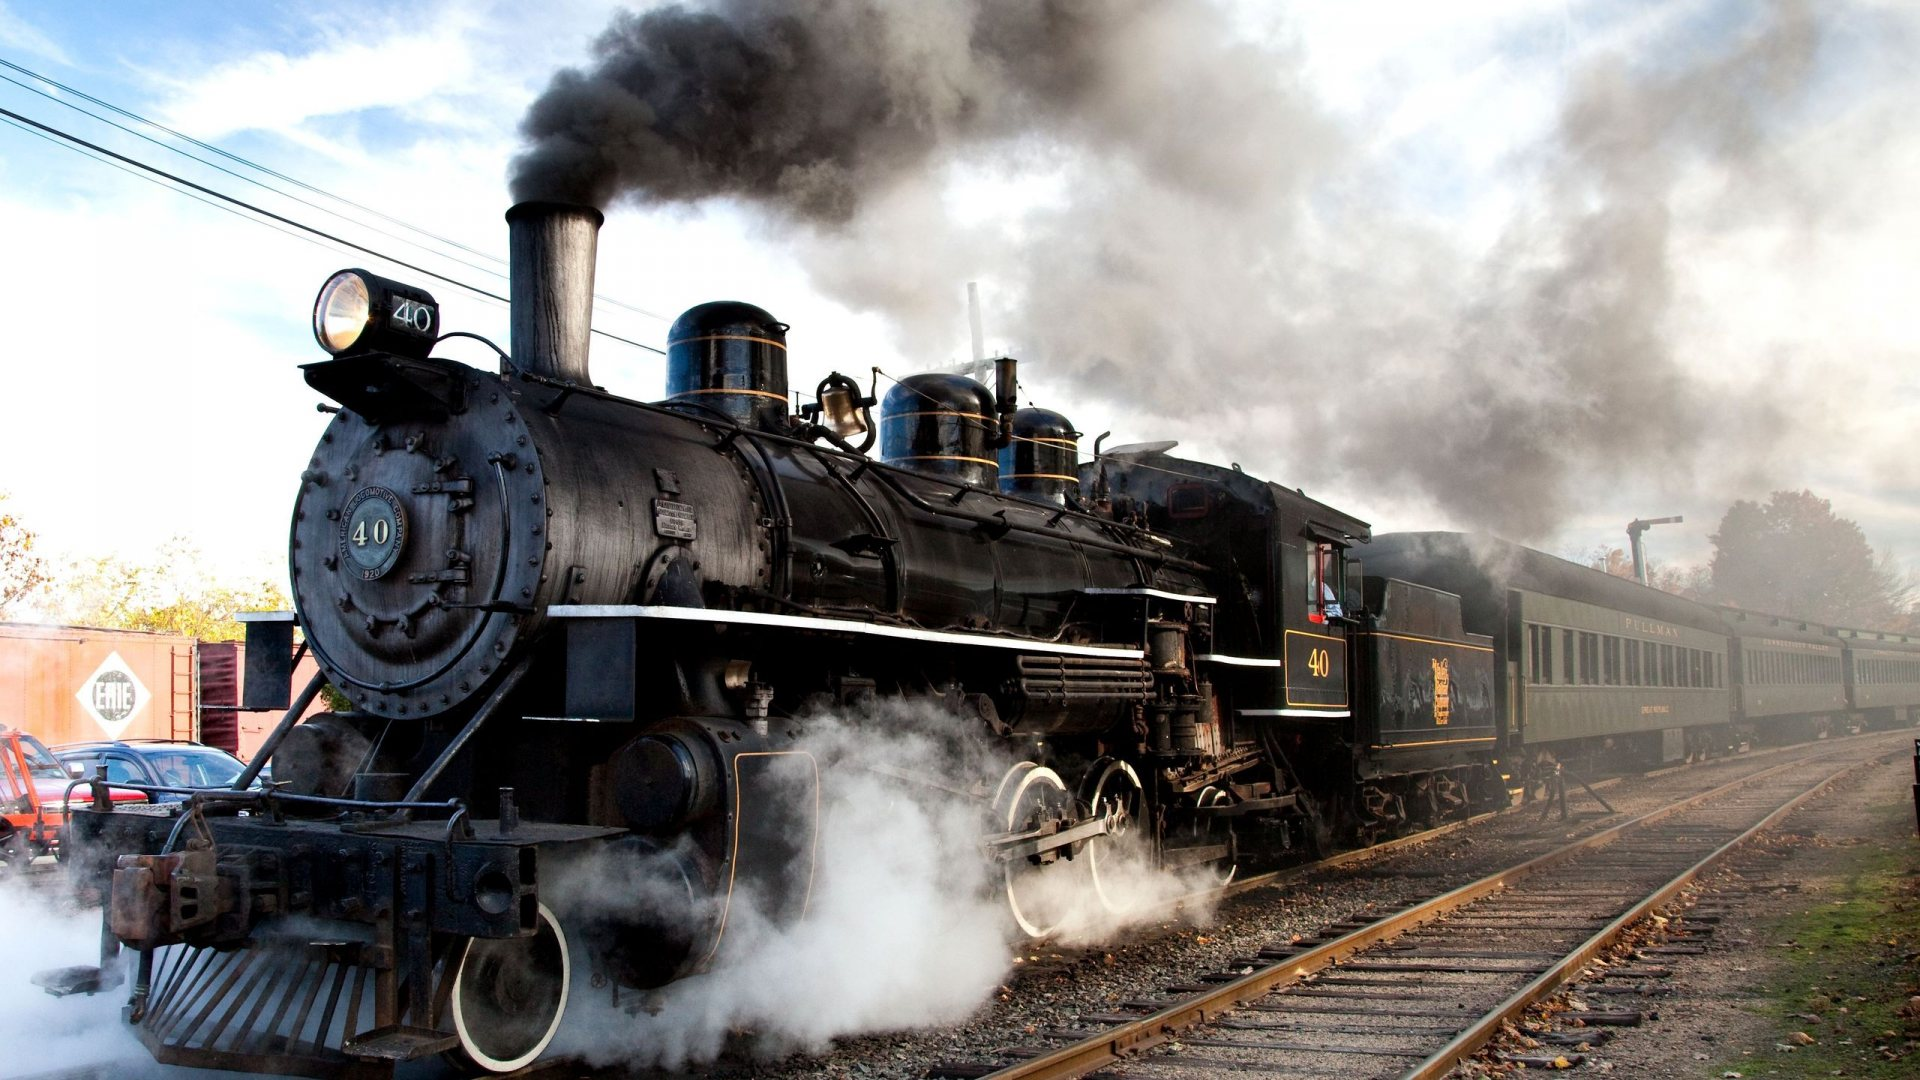
\includegraphics[width=\paperwidth,height=\paperheight,%
			keepaspectratio]{img/train.jpg}%
			\vfill
}}}


\begin{document}

\AddToShipoutPicture*{\BackgroundPic}

\frenchspacing % Reduces space after periods to make text more compact

\raggedbottom % Makes all pages the height of the text on that page

\selectlanguage{italian}

\pagenumbering{roman} % Roman page numbering prior to the start of the thesis content (i, ii, iii, etc)

\pagestyle{plain} % Suppress headers for the pre-content pages

%-------------------------------------------------------------------
%	Frontespizio-Indice
%-------------------------------------------------------------------

% Title Page

\begin{titlepage}

\begin{addmargin}[-1cm]{-3cm}
\begin{center}
\large

\hfill
\vfill

\begingroup
\color{Maroon}\spacedallcaps{Monitoraggio selettivo di stazioni e tratte ferroviarie in base alla loro esposizione alla pericolosità di frana: un approccio GIS} \\ \bigskip
\endgroup

\spacedlowsmallcaps{Caruso Federica}
\\
\spacedlowsmallcaps{Di Sabatino Fabio}
\\
\spacedlowsmallcaps{Giancola Davide}
\vfill






\end{center}
\end{addmargin}
\end{titlepage} % Main title page
\cleardoublepage
\cleardoublepage% Table of Contents - List of Tables/Figures/Listings and Acronyms

\refstepcounter{dummy}

\pdfbookmark[1]{\contentsname}{tableofcontents} % Bookmark name visible in a PDF viewer

\setcounter{tocdepth}{2} % Depth of sections to include in the table of contents - currently up to subsections

\setcounter{secnumdepth}{3} % Depth of sections to number in the text itself - currently up to subsubsections

\manualmark
\markboth{\spacedlowsmallcaps{\contentsname}}{\spacedlowsmallcaps{\contentsname}}
\tableofcontents 
\automark[section]{chapter}
\renewcommand{\chaptermark}[1]{\markboth{\spacedlowsmallcaps{#1}}{\spacedlowsmallcaps{#1}}}
\renewcommand{\sectionmark}[1]{\markright{\thesection\enspace\spacedlowsmallcaps{#1}}}

\clearpage

\begingroup 
\let\clearpage\relax
\let\cleardoublepage\relax
\let\cleardoublepage\relax

%----------------------------------------------------------------------------------------
%	List of Figures
%----------------------------------------------------------------------------------------

\refstepcounter{dummy}
%\addcontentsline{toc}{chapter}{\listfigurename} % Uncomment if you would like the list of figures to appear in the table of contents
\pdfbookmark[1]{\listfigurename}{lof} % Bookmark name visible in a PDF viewer

\listoffigures

\vspace{8ex}
\newpage
        

 
                   
\endgroup % Contents, list of figures/tables/listings and acronyms

\cleardoublepage

\pagenumbering{arabic} 

\cleardoublepage % Avoids problems with pdfbookmark

%----------------------------------------------------------------------------------------
%	Contenuto della relazione
%----------------------------------------------------------------------------------------

\chapter{Introduzione}

\label{ch:introduzione}
La mobilità delle persone e delle merci sono una componente essenziale del mercato interno dell'Unione Europea (UE) ed è di fondamentale importanza garantire la sua fattibilità al fine di salvaguardare la crescita economica.
La rete ferroviaria ha un ruolo strategico in questo contesto almeno sotto due punti di vista:
\begin{enumerate}
\item Offre un impulso rilevante all'integrazione e all'efficienza dell'economia dell'UE.
\item Facilita il libero movimento delle persone e delle merci garantendo una modalità di trasporto efficiente e sostenibile dal punto di vista ambientale. Secondo l’Agenzia europea dell’ambiente, le emissioni di $CO_2$ provenienti dal trasporto ferroviario sono
3,5 volte inferiori, per tonnellata-chilometro, a quelle prodotte dal trasporto su strada. Di conseguenza, promuovere modalità di trasporto come quello su rotaia, piuttosto che su strada, permetterebbe all'UE di essere meno dipendente dall'importazione di petrolio e di ridurre l'inquinamento.
\end{enumerate}

Alla luce di queste considerazioni preliminari non sorprende che la sicurezza assumi un rilievo crescente in questo contesto; Una testimonianza di ciò è il regolamento su un metodo comune di sicurezza (CSM) per la valutazione del rischio e l’accertamento, rilasciato negli ultimi anni dall’agenzia ferroviaria europea (ERA) e dalla Commissione Europea [Regulation EU, No.402/2013, 2015].
Un recente regolamento [GE/GN8642, 2014] pubblicato dalla Rail Safety and Standards Board Ltd (http://www.rssb.co.uk/) definisce “\textit{un pericolo, come una condizione che potrebbe portare a un incidente}”. A sua volta, la direttiva sulla sicurezza [2004/49/CE] del Parlamento europeo definisce un incidente come: “\textit{per 'incidente' si intende un evento improvviso indesiderato e non intenzionale o specifica catena di siffatti eventi aventi conseguenze dannose. Gli incidenti sono suddivisi nelle seguenti categorie: collisioni, deragliamenti, incidenti ai passaggi a livello, incidenti a persone causati da materiale rotolante in movimento, incendi ed altri.}”\newline

Nel tempo sono stati sviluppati molti metodi per predire, prevenire e ridurre il numero di incidenti e per aumentare la sicurezza nel contesto ferroviario. Inoltre è fondamentale sottolineare il fatto che le tratte e le relative stazioni insistono su un territorio esposto, tra gli altri, al rischio idrogeologico. Di riflesso anche la rete ferroviaria e le relative stazioni che su di esso insistono lo sono. I deragliamenti dei treni sono il rischio principale di incidenti. [Lloyd et al., 2001], [Manning et al., 2008], [He et al., 2011] sono esempi di studi che hanno affrontato la questione. In tali studi si fa uso di metodi matematici classici. Ad esempio, [He et al. (2011)] fanno ricorso alla Principal Component Analysis per identificare un numero limitato di fattori che devono essere presi in considerazione per studiare la stabilità dei pendii rocciosi. Studi teorici come quelli appena citati sono molto interessanti perché aiutano a comprendere la complessità del problema, fornendo delle informazioni globali circa le variabili in gioco e come esse sono correlate, ma hanno il limite di non essere direttamente traducibili in piani di lavoro attuabili da parte di coloro che hanno responsabilità di garantire la sicurezza delle tratte ferroviarie e le relative stazioni.\newline

Nel nostro documento si adotta un approccio differente, basato su metodi proposti nell'ambito della Geographical Information Science e riferiti allo studio di relazioni topologiche tra caratteristiche geografiche. Come vedremo, facendo ricorso a tali metodi, possibile identificare quali sono le potenziali pericolosità delle tratte ferroviarie e delle relative stazioni determinate dalle caratteristiche morfologiche e litologiche del terreno dove sono situate, dalla sua pendenza nonché dall'uso dello stesso (prevalentemente abitativo, prevalentemente ad uso coltivazione, ecc).\newline 

Le frane costituiscono uno dei più importanti rischi naturali in molti paesi in tutto il mondo, [Brabb e Harrod, 1989]. Questo è il caso dell’Italia, dove le frane sono diffuse e provocano notevoli danni e decessi ogni anno, [Guzzetti, Stark, e Salvati, 2005], [Trigila et al., 2010]. Secondo il risultato di un recente studio effettuato da [Jaedicke et al. (2014)], “\textit{l'Italia ha il più alto numero di persone esposte al pericolo di frana tra i paesi europei.}”\newline

Mantenendosi ad un alto livello di astrazione quello che si può anticipare del metodo che ci si accinge a presentare è che esso consente di fare delle valutazioni circa le potenziali pericolosità delle tratte ferroviarie e delle relative stazioni che insistono sul territorio oggetto di studio. Ciò consente di restituire agli utenti finali informazioni dettagliate per la localizzazione delle porzioni di tratte ferroviarie e delle stazioni ove prioritariamente è opportuno fare dei controlli periodici.
La strategia proposta quindi supera i limiti posti dai controlli periodici sull'intero percorso ferroviario e su tutte le stazioni situate sul territorio, i quali risultano essere lunghi e, di conseguenza, costosi e non sempre utili come sostenuto da [Sadler et al., (2016)]. Utilizzando tale metodo sarà possibile individuare quali sono le porzioni di tratte ferroviarie e le stazioni le cui misure di controllo possono essere ridotte in modo sicuro, permettendo al settore ferroviario significativi risparmi di costi a favore del potenziamento dei controlli di porzioni di tratte ferroviarie e stazioni che hanno una pericolosità potenziale maggiore.\newline

In sintesi, obiettivo dello studio metodologico-sperimentale descritto in questo documento è sviluppare una metodologia scientificamente robusta per l’identificazione degli hotspot ferroviari ad alto rischio e che sia di supporto nella definizione di una strategia di monitoraggio selettiva dello stato di sicurezza per una categoria di beni strategica per un Paese, ovvero la sua rete ferroviaria, rispetto all'esposizione della stessa ai movimenti franosi.\newline

Le tratte ferroviarie e le relative stazioni sono dunque i due target da proteggere e data la loro diversa connotazione spaziale che le descrive vanno trattate ed analizzate separatamente. Infatti, le tratte sono modellabili con la geometria \textit{linea}, mentre le stazioni sono modellabili con la geometria \textit{punto}.\newline

Lo strumento software da noi sviluppato è basato sull'uso di un Geo-DB arricchito con un ampio numero di User Defined Functions (UDF), tramite le quali è possibile effettuare delle elaborazioni complesse scrivendo delle queries SQL semplici alla portata della maggior parte dei tecnici che lavorano nel settore della sicurezza ferroviaria.

$\{$ \textit{Continuare...} $\}$

Il documento è organizzato come segue: nella Sezione 2 viene mostrata una panoramica degli strumenti e gli algoritmi utilizzati per valutare l’esposizione al rischio di frana delle stazioni ferroviarie dislocate sul territorio.

$\{$ \textit{Continuare...} $\}$

Il metodo proposto sarà sperimentato con riferimento alla rete ferroviaria Italiana dislocata all'interno del territorio della regione Abruzzo (Italia Centrale).
\chapter{Materials and methods } % Chapter title

\label{ch:materialandmethods} % For referencing the chapter elsewhere, use \autoref{ch:examples} 

%----------------------------------------------------------------------------------------

\section{Notazioni}
\label{notazioni}
Da qui in poi useremo le seguenti notazioni:
\begin{enumerate}


\item \textit{GeoArea}: Porzione di territorio di interesse per lo studio. La \textit{GeoArea} può coincidere con un comune, una provincia, una regione, una nazione o un intero continente. Nel nostro caso di studio si tratta della regione Abruzzo (fig. \ref{fig:abruzzo}).
\begin{figure}[h]
	\centering		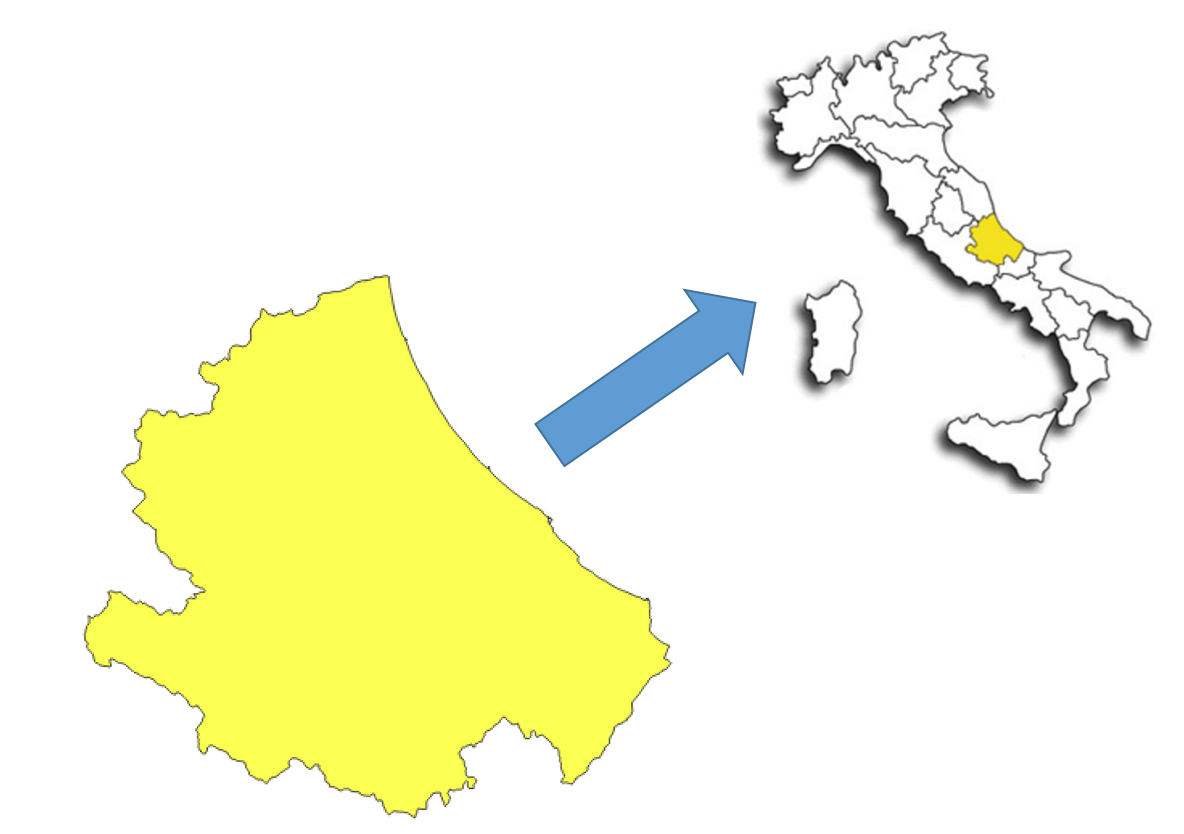
\includegraphics[width=0.5\textwidth]{img/abruzzo}
	\caption{La nostra \textit{GeoArea}: La regione Abruzzo}
    	\label{fig:abruzzo}
\end{figure}

La \textit{GeoArea} viene descritta dalla seguente tupla: <gid, geom>.
\begin{itemize}
\item \textit{gid}: Identificativo numerico univoco del territorio.
\item \textit{geom}: Rappresentazione geometrica del territorio (\textit{MultiPolygon}).
\end{itemize}
%------------------------------------------------

\item\textit{Z}=$\{${$z_k$}, k=1,2,..$\}$ dove $z_k$ denota una zona k-esima della \textit{GeoArea}, ognuna caratterizzata da un insieme di informazioni territoriali. L'insieme \textit{Z} è una partizione della \textit{GeoArea}, ovvero è una collezione di elementi $z_k$, non nulli, tali da avere intersezione vuota a due a due e tali che la loro unione coincida con l'intera \textit{GeoArea}, per maggiore chiarezza si rimanda alla fig. \ref{fig:geoarea}.  
\begin{figure}[h]
\centering
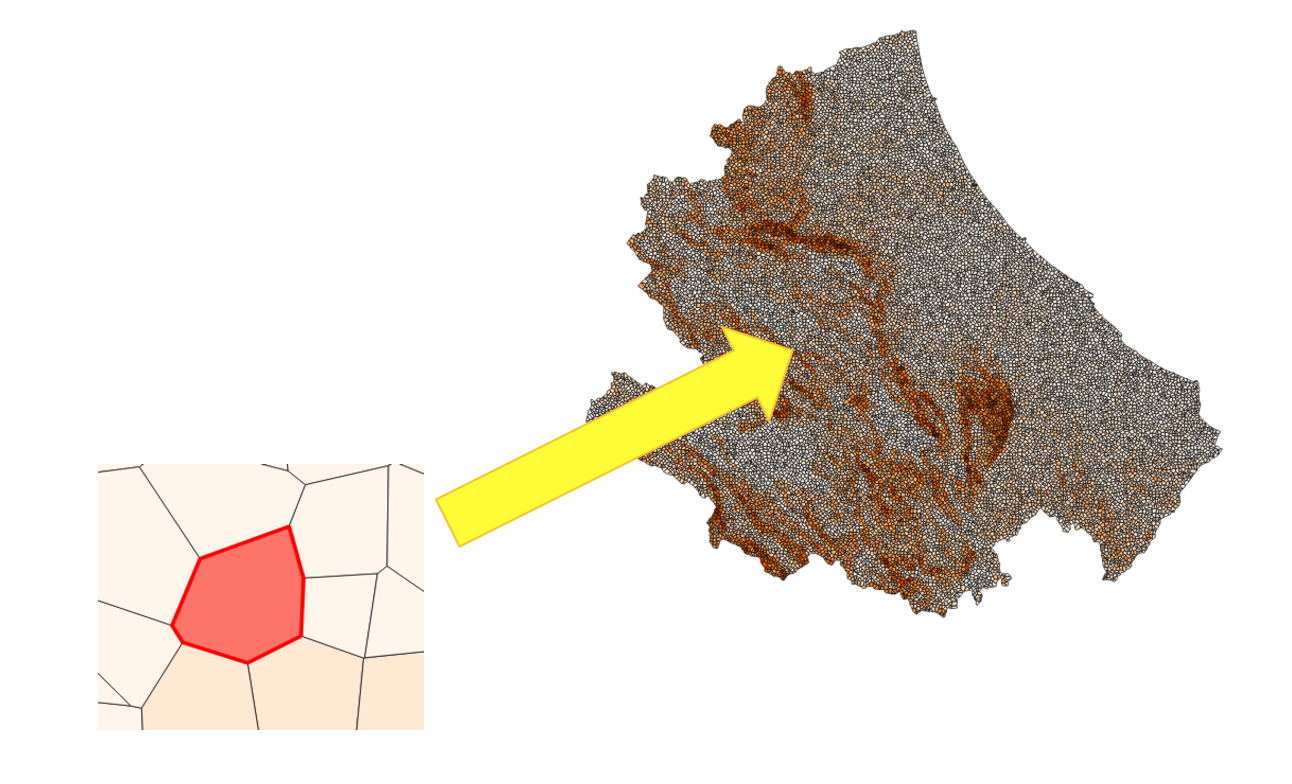
\includegraphics[width=0.5\textwidth]{img/zeta}
\caption{Generico elemento $z_k$ dell'insieme \textit{Z}}
	\label{fig:geoarea}
\end{figure}
\newpage
Il generico elemento di \textit{Z} (i.e. $z_k$) è definito mediante la tupla: <gid, $S_{zk}$, geom, \textit{avgElevation}>.
\begin{itemize}
\item \textit{gid}: Identificativo numerico univoco dell'elemento $z_k$.
\item \textit{$Sz_k$}: Valore numerico che quantifica la pericolosità di frana dell'elemento $z_k$. 
\item \textit{geom}: Rappresentazione geometrica del \textit{boundary} dell'elemento $z_k$.

\item \textit{avgElevation}: Altitudine media dell'elemento $z_k$, ottenuta mediante una media ponderata delle altitudini delle curve di livello che intersecano, almeno in parte, l'elemento $z_k$. Il modo in cui verrà calcolato questo valore verrà descritto nel dettaglio nella notazione successiva di $\Delta{h}$ poiché bisogna prima introdurre ulteriori concetti.
\end{itemize}
Si noti che $z_k$ è una notazione sovraccaricata dato che rappresenta sia il \textit{gid} della zona che la sua geometria.
%------------------------------------------------

\item\textit{B}=$\{$ $b_i$, i=1,2,... $\}$ dove $b_i$ indica l'edificio della stazione (\textit{B} sta per \textit{Station Building}) contenuta nel \textit{boundary} della \textit{GeoArea}. Di questo edificio non teniamo conto della sua conformazione architettonica, della sua altezza o del numero di piani della struttura poiché spesso sono delle informazioni che difficilmente sono reperibili ma bensì consideriamo la sua posizione geografica, espressa da una coppia di coordinate, informazione spesso nota. Un esempio di un generico elemento $b_i$ è rappresentato in fig. \ref{fig:b}.
\newpage
\begin{figure}[bht]
\centering
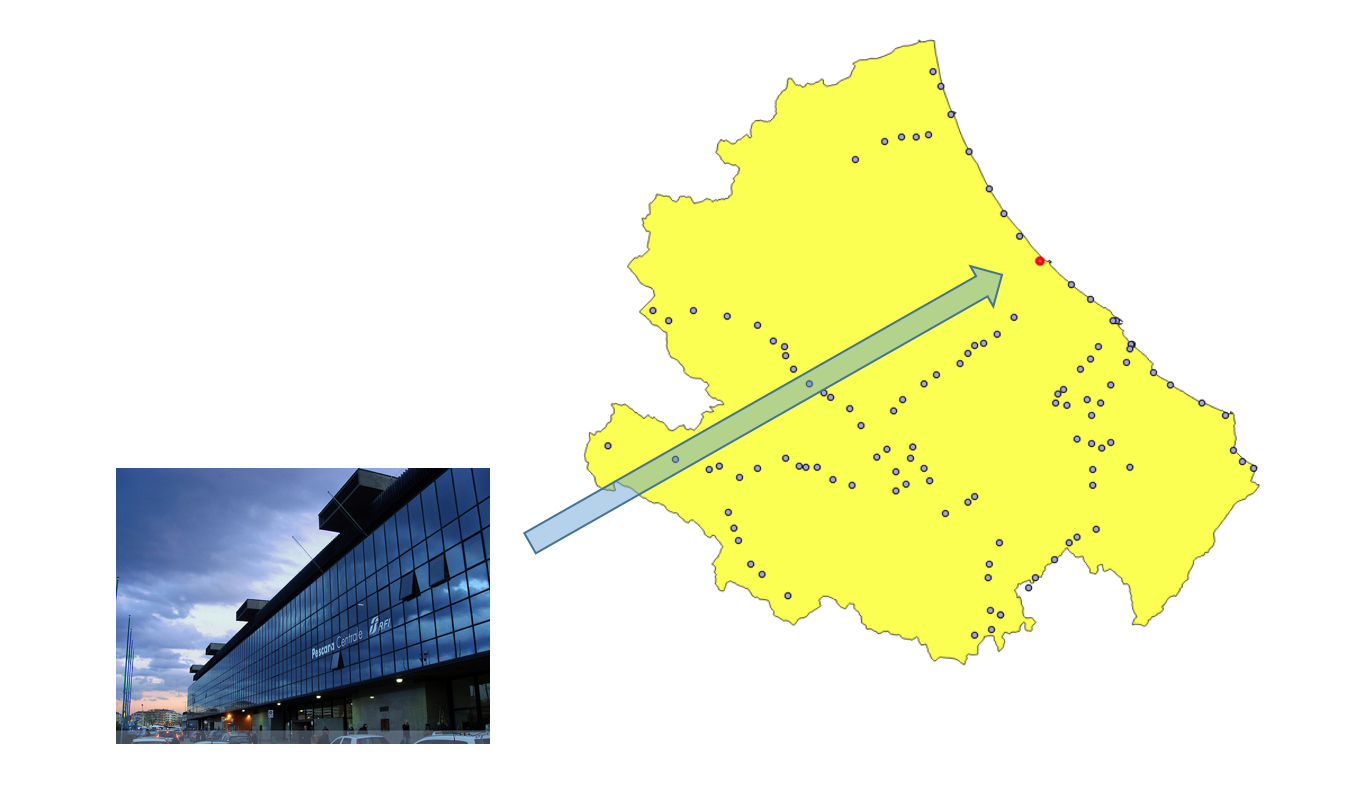
\includegraphics[width=0.5\textwidth]{img/stazionegenerica}
\caption{Generico elemento $b_i$ dell'insieme \textit{B}}
	\label{fig:b}
\end{figure}

Il generico elemento di \textit{B} (i.e. $b_i$) è definito mediante la tupla: <gid, name, geom, \textit{$Exp\_b_i$}, \textit{elevation}>.
\begin{itemize}
\item \textit{gid}: Identificativo numerico univoco dell'elemento $b_i$.
\item \textit{name}: Nome testuale dell'i-esimo elemento dell'insieme \textit{B}, espresso tramite una stringa.
\item \textit{geom}: Rappresentazione geometrica (\textit{Point}) dell'elemento $b_i$.
\item \textit{Exp$\_$$b_i$}: Grado di esposizione al pericolo di frana del generico elemento $b_i$, determinato da tutte le $z_k$ in \textit{Z}.
\item \textit{elevation}: Altitudine espressa in metri a cui si trova il generico elemento $b_i$.
\end{itemize}
Si noti che $b_i$ è una notazione sovraccaricata dato che rappresenta sia il \textit{gid} della stazione ferroviaria che la sua geometria.
%------------------------------------------------
\item\textit{E}=$\{$ $e_j$, j=1,2,... $\}$ dove $e_j$ denota una curva di livello contenuta almeno in parte nel \textit{boundary} della \textit{GeoArea}. In geografia, con particolare riguardo alla cartografia, la curva di livello è quella curva che unisce punti con uguale quota (figura 4(b)), ovvero uguale distanza verticale dal piano di riferimento al quale è stato attribuito quota zero; se sono sopra il livello del mare si chiameranno \textit{isoipse} (dal greco ísos = "uguale" e hýpsos = "altezza") mentre al contrario \textit{isobate} (dal greco ísos = "uguale" e báthos = "profondità"). Nella figura 4(a) è possibile vedere un esempio di $e_j$.

\begin{figure}[bth]
\myfloatalign
\subfloat[]
{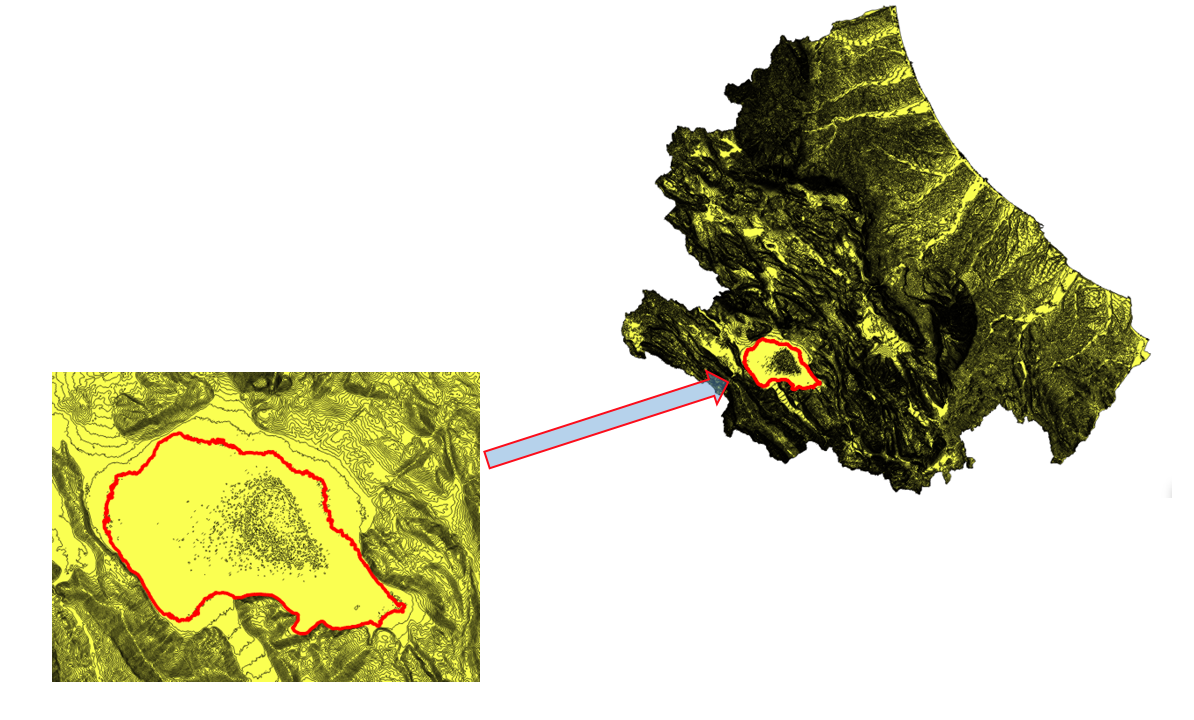
\includegraphics[width=.45\linewidth]{img/curva}} \quad
\subfloat[]
{\label{fig:example-b}
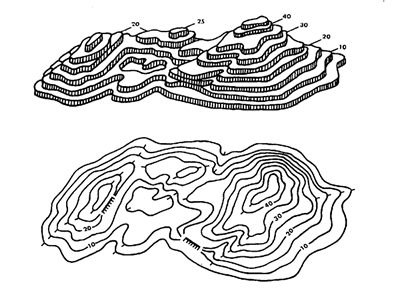
\includegraphics[width=.45\linewidth]{img/esempioLivello}} \\
\label{fig:example}
\caption{(a) Generico elemento $e_j$ dell'insieme; (b)Esempio di curve di livello per un certo territorio }
\end{figure}


Ogni elemento dell'insieme \textit{E} (i.e. $e_j$) è definito mediante la tupla: <gid, elevation, geom>.
\begin{itemize}
\item \textit{gid}: Identificativo numerico univoco dell'elemento $e_j$.
\item \textit{elevation}: Valore numerico che rappresenta la quota espressa in metri dell'elemento $e_j$.
\item \textit{geom}: Rappresentazione geometrica (\textit{MultiLineString}) dell'elemento $e_j$.
\end{itemize}
Si noti che $e_j$ è una notazione sovraccaricata dato che rappresenta sia il \textit{gid} della curva di livello che la sua geometria.
%------------

\item\textit{buffer$_i$}=buffer($b_i$,$r$) rappresenta una geometria costituita da tutti i punti la cui distanza dal punto $b_i$ risulta essere minore o uguale del raggio $r$. Nella figura \ref{fig:bufferi} è possibile vedere un esempio di $buffer_i$.
\begin{figure}[bht]
\centering
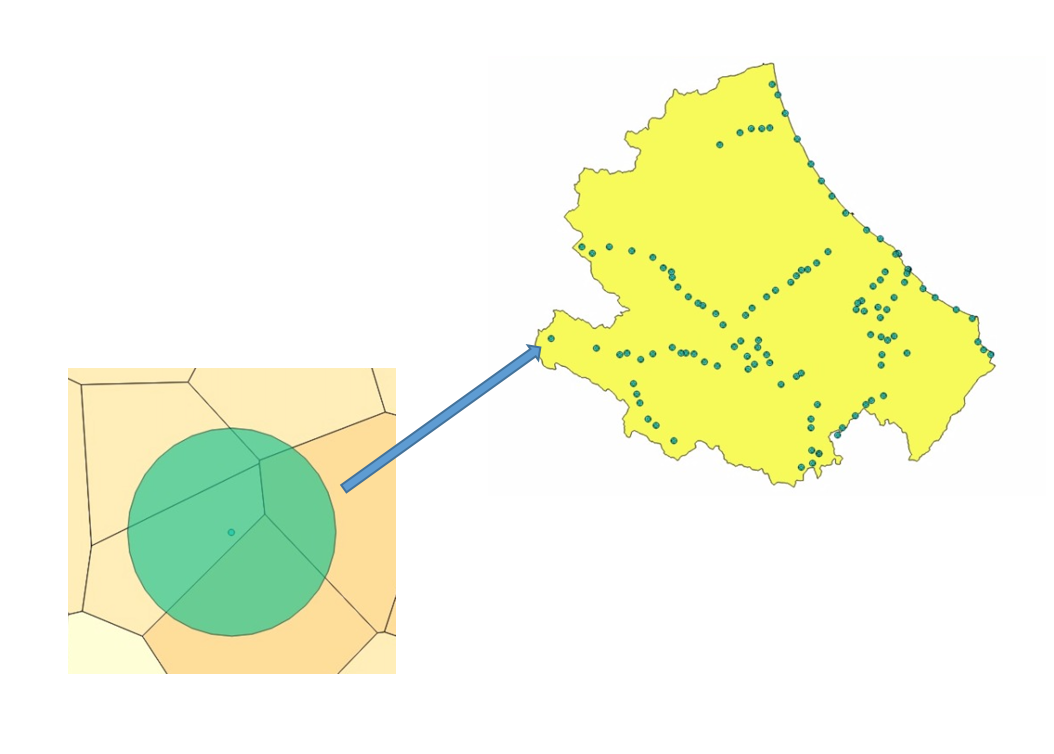
\includegraphics[width=0.5\textwidth]{img/buffer}
\caption{Esempio di $buffer_i$ costruito su una generica $b_i$}
\label{fig:bufferi}
\end{figure}
%-----------
\newpage
\item\textit{V}=$\{$$v_\gamma$ ($\gamma$=1,2,...) := $z_k$ $\in$ \textit{Z} | $buffer_i$ $\cap$ $z_k$ $\neq$ $\emptyset$ $\}$ è l'insieme di tutte le $z_k$ contenute nella \textit{GeoArea} che intersecano almeno in parte \textit{$buffer_i$}. La cardinalità di tale insieme è pari a $N$. Un esempio di insieme $V$ è osservabile nella fig. \ref{fig:v}.
\begin{figure}[bht]
\centering
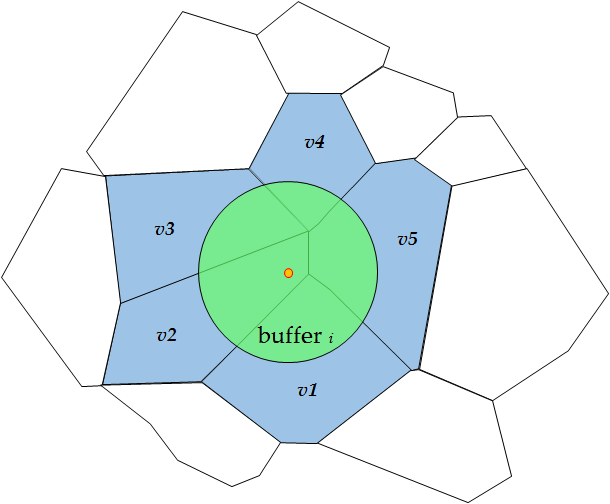
\includegraphics[width=0.5\textwidth]{img/V}
\caption{V=$\{$$v_1$, $v_2$, $v_3$, $v_4$, $v_5$ $\}$}
\label{fig:v}
\end{figure}
%-----------

\item\textit{P}=$\{$$p_m$ (m=1,2,..) := $buffer_i$ $\cap$ $e_j$ $\neq$ $\emptyset$, $\forall$ $e_j$ $\in$ \textit{E}$\}$ è l'insieme dei segmenti delle curve di livello, determinati dall'intersezione tra le curve di livello contenute nell'insieme \textit{E} e il $buffer_i$. In figura \ref{fig:p} è riportato un esempio di insieme $P$.
\begin{figure}[h]
\centering
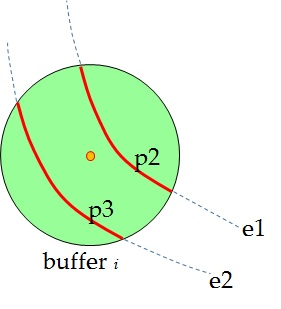
\includegraphics[width=0.4\textwidth]{img/P}
\caption{P=$\{$$p_2$, $p_3$$\}$}
\label{fig:p}
\end{figure}
%-----------
\newpage
\item\textit{T}=$\{$$t_f$ (f=1,2,...) := $v_\gamma$ $\cap$ $e_j$ $\neq$ $\emptyset$, $\forall$ $e_j$ $\in$\textit{E}, $\forall$ $v_\gamma$$\in$\textit{V}$\}$ è l'insieme dei segmenti delle curve di livello, determinati dall'intersezione tra le curve di livello contenute nell'insieme \textit{E} e le zone $v_\gamma$ contenute nell'insieme \textit{V}. In fig. \ref{fig:t} è possibile osservare un esempio di insieme T.
\begin{figure}[h]
\centering
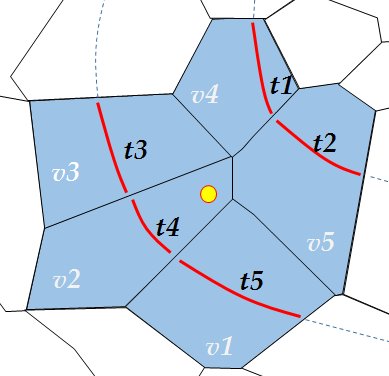
\includegraphics[width=0.4\textwidth]{img/T}
\caption{T=$\{$$t_1$, $t_2$, $t_3$, $t_4$, $t_5$ $\}$}
\label{fig:t}
\end{figure}
%-----------

\item $\Delta{h}$ è così definito:
\begin{equation}
 \Delta{h} =  | h\_stazione - h\_media\_v_\gamma |
 \end{equation}
Dove: 
\begin{itemize}
\item $ h\_stazione$ indica l'\textit{elevation} dell'edificio $b_i$
\item $ h\_media\_v_\gamma$ indica l'\textit{avgElevation} media di $v_\gamma$
\end{itemize}
Il metodo di calcolo dell'elevation per gli edifici e le zone è diverso. Infatti qui di seguito descriveremo le diverse modalità di calcolo:
\begin{enumerate}
\item h\_media\_$v_\gamma$ : l'\textit{elevation} delle v$_\gamma$ viene calcolata effettuando la media aritmetica dell'elevation delle curve di livello che intersecano $v_\gamma$.

\begin{figure}[h]
  \centering
    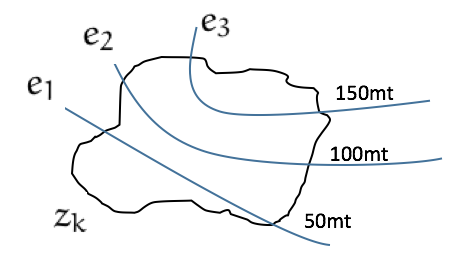
\includegraphics[width=0.5\textwidth]{img/altezzaZK}
      \caption{Esempio di una $v_\gamma$ con tre curve di livello}
      \label{fig:altezzaZK}
\end{figure}
Ad esempio, in fig.\ref{fig:altezzaZK} la quota media di $v_\gamma$ risulta essere: \newline
$\frac{50\ +\ 100\ +\ 150}{3} = 100 mt$

\item $h\_{stazione}$: il calcolo dell'\textit{elevation} per gli edifici è più sofisticato ma permette di ottenere valori molto accurati.
Le possibili situazioni che si possono presentare sono tre e verranno analizzate qui di seguito:
\begin{itemize}
\item edificio racchiuso da un'unica curva di livello (Fig.10) oppure in prossimità del confine della \textit{GeoArea} (Fig.11). Si definisce un edificio di questo tipo come edificio in posizione "atipica".

\begin{figure}[bth]
\myfloatalign
\subfloat[]
{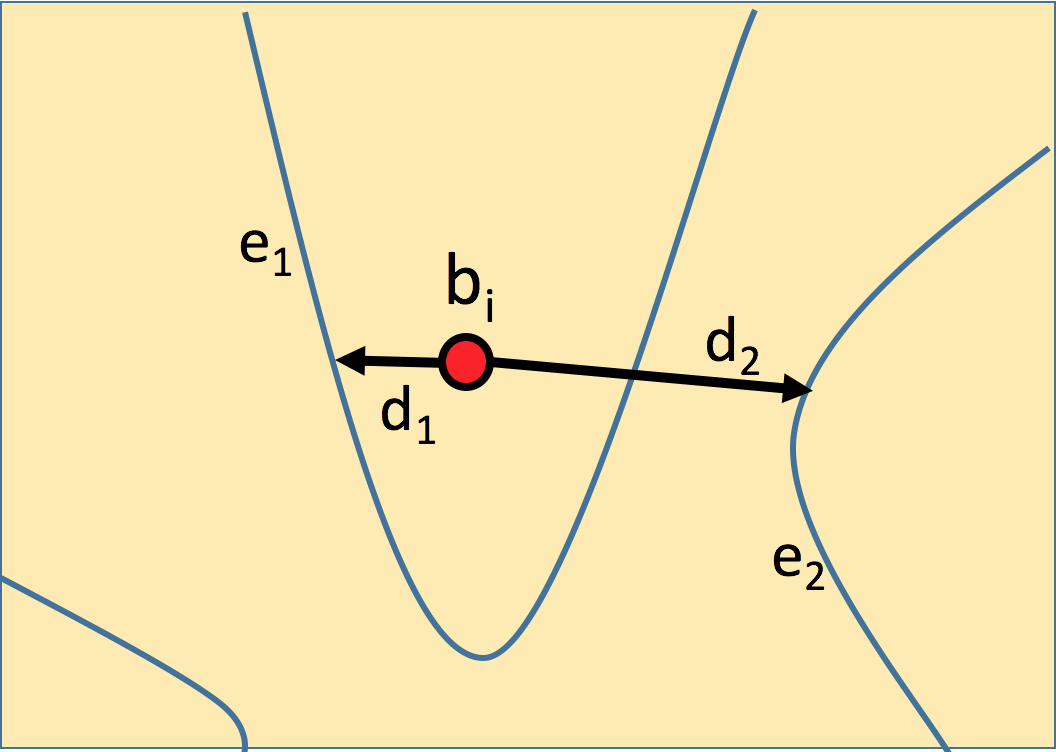
\includegraphics[width=.45\linewidth]{img/unalinea}} \quad
\subfloat[]
{\label{fig:unalinea-a}
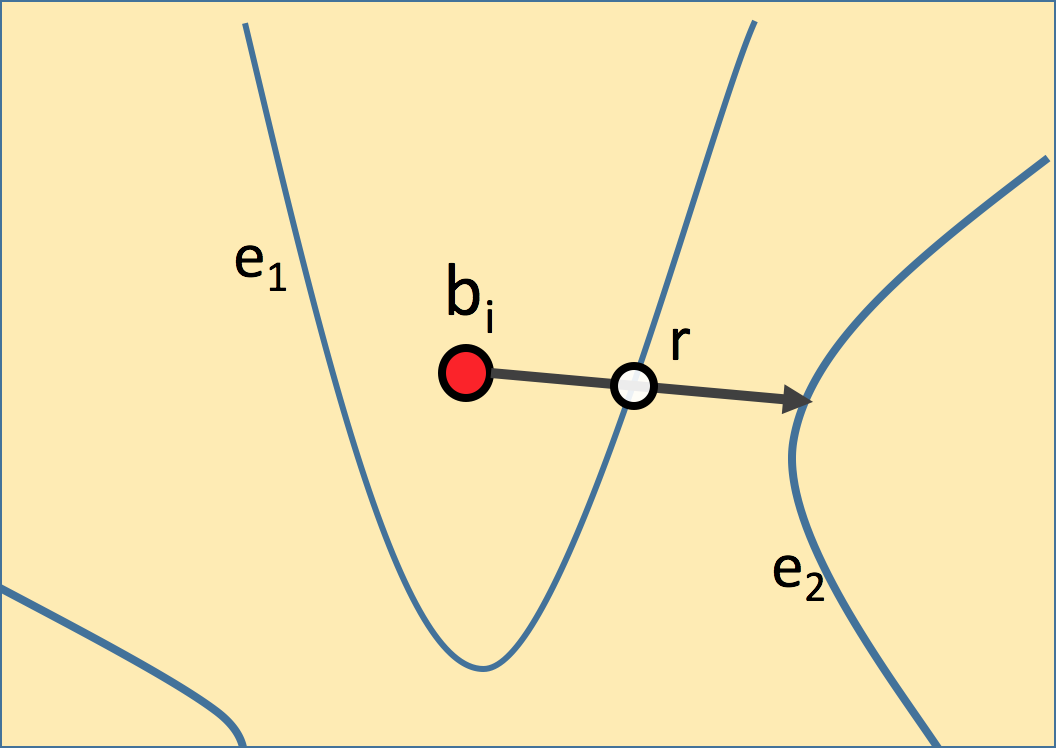
\includegraphics[width=.45\linewidth]{img/unalinea2}} 
\caption[]{Edificio racchiuso da un'unica curva di livello.}\label{fig:unalinea}
\end{figure}

\begin{figure}[bth]
\myfloatalign
\subfloat[]
{\label{fig:confine-a}
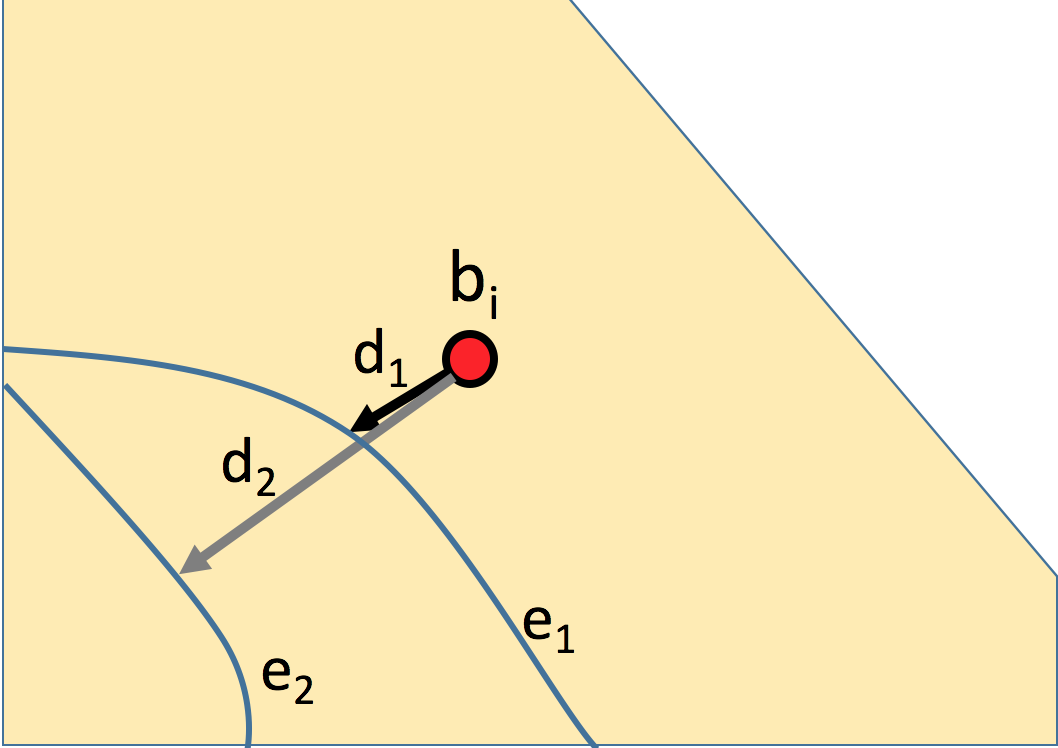
\includegraphics[width=.45\linewidth]{img/lineaconfine}} \quad
\subfloat[]
{\label{fig:confine-b}
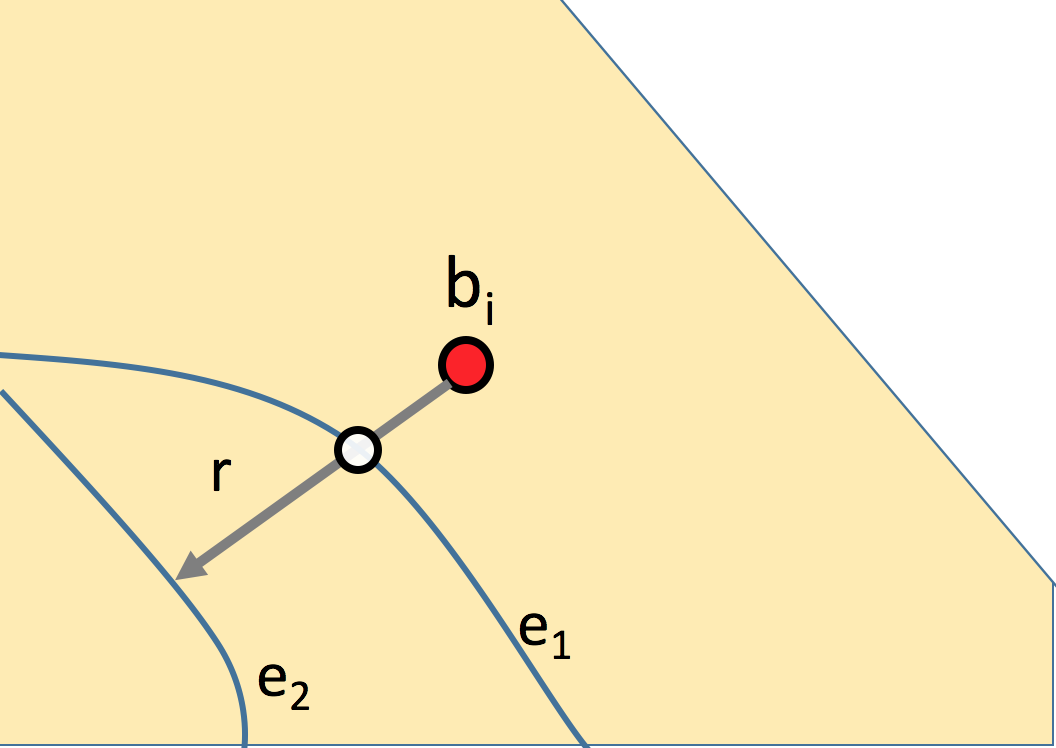
\includegraphics[width=.45\linewidth]{img/lineaconfine2}} 
\caption[]{Edificio in prossimità del confine della \textit{GeoArea}.}\label{fig:confine}
\end{figure}

Entrambi i casi vengono rilevati nel medesimo modo, ovvero tracciando la semiretta avente come origine l'edificio $b_i$ (pallino rosso) e passante per la curva $e_2$. Se la semiretta interseca anche $e_1$, allora ci troviamo in una delle situazioni esplicate in Fig.\ref{fig:unalinea} (b) e in Fig. \ref{fig:confine} (b). Quindi $h\_stazione$ equivale all'\textit{elevation} della curva di livello $e_1$, supponendo che $d_1 < d_2$.

\newpage

\item Edificio circondato da due curve di livello come in Fig.\ref{fig:circondata}. Si definisce un edificio di questo tipo come edificio in posizione "tipica".

\begin{figure}[bth]
\myfloatalign
\subfloat[]
{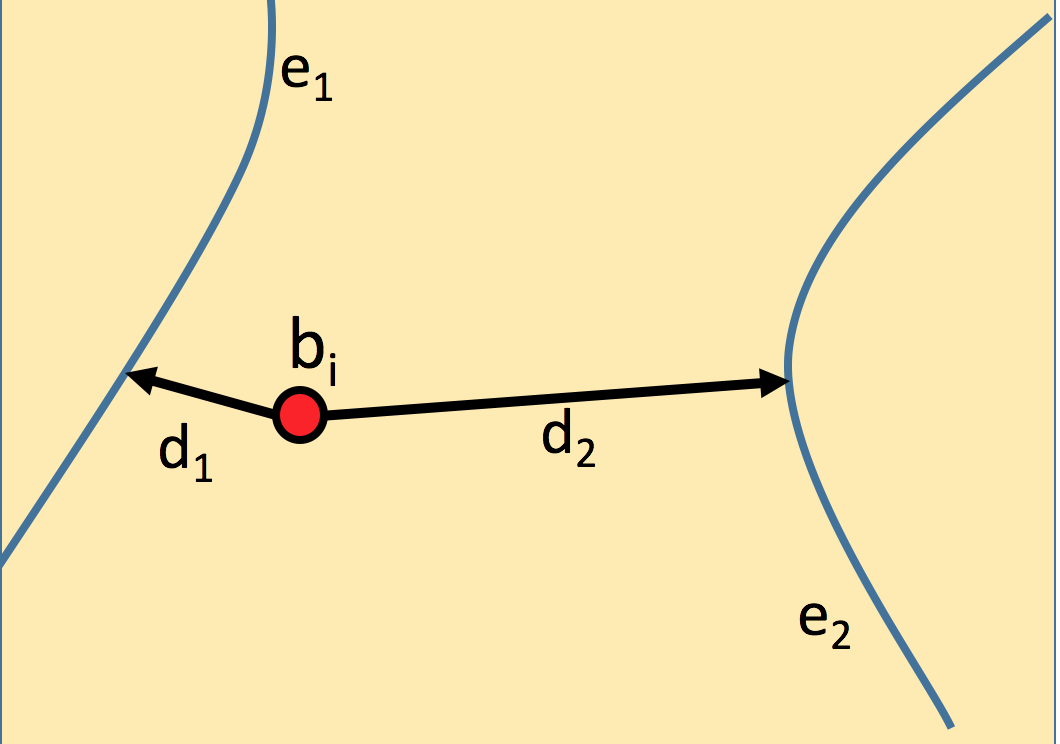
\includegraphics[width=.45\linewidth]{img/duelinee-a}} \quad
\subfloat[]
{\label{fig:circondata-b}
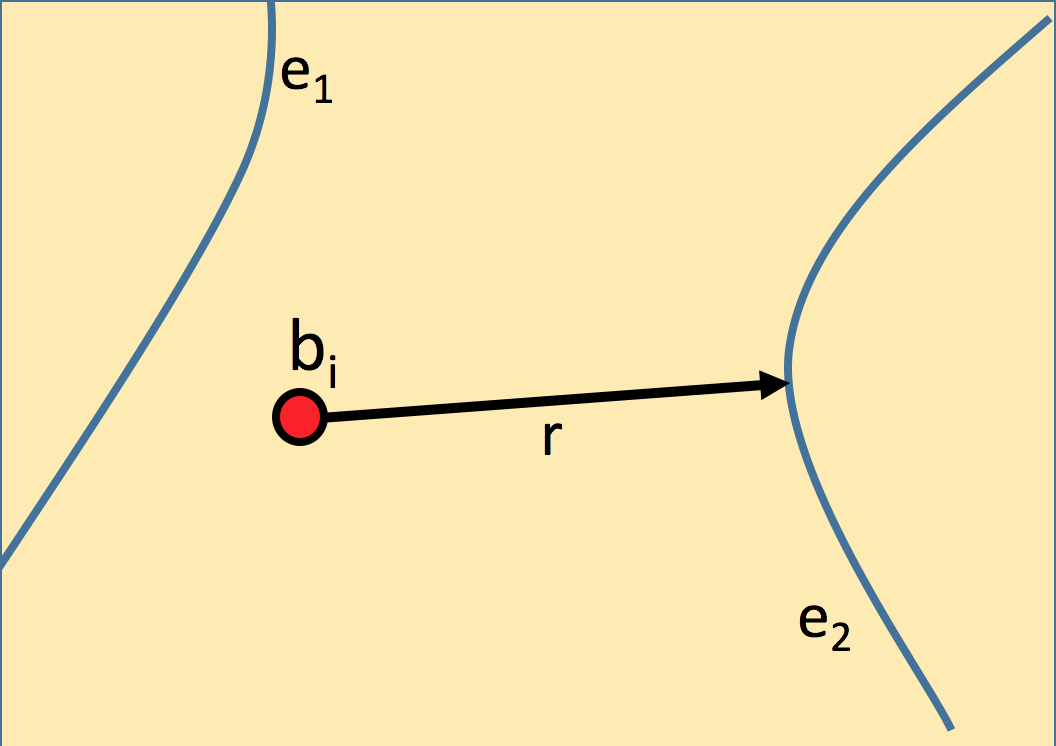
\includegraphics[width=.45\linewidth]{img/duelinee-b}} 
\caption[]{Edificio in prossimità del confine della \textit{GeoArea}.}\label{fig:circondata}
\end{figure}

Dalla Fig.\ref{fig:circondata} (b) si evince che, a differenza delle situazioni esplicate dalle Fig.\ref{fig:unalinea} (b) e Fig.\ref{fig:confine} (b), la semiretta avente origine in $b_i$ e passante per $e_2$ non interseca la curva di livello $e_1$.
Dunque $h\_stazione$ è così definito:
\begin{equation}
\label{eq:hstazione}
   h\_stazione = \frac{(h\_e_1 \times d_2) \times ( h\_e_2 \times d_1)}{d_1 +d_2}
\end{equation}
Dove:
\begin{itemize}
\item $h\_e_j$ indica l'\textit{elevation} della curva di livello $e_j$, con $j=1,2$
\item $d_j$ indica la distanza tra l'edificio $b_i$ e la curva di livello $e_j$ con $j=1,2$
\end{itemize}

L'Eq.\ref{eq:hstazione} è una media ponderata delle quote delle due curve di livello più vicine all'edificio $b_i$. Al numeratore le distanze vengono utilizzate come pesi della media, affinché la quota della curva $e_1$, più vicina all'edificio $b_i$, risulti più determinante nel calcolo della $h\_stazione$ rispetto alla quota della curva $e_2$.
\end{itemize}
\end{enumerate}

\item \textit{Azimuth}:
L'azimuth è la coordinata orizzontale angolare espressa dall'arco d'ortodromia della sfera celeste che si forma partendo convenzionalmente dal punto cardinale nord fino all'oggetto di osservazione,muovendosi in senso orario verso est, quindi a sud e a ovest, fino a tornare al punto di inizio a nord (cioè un angolo giro, 360° sessagesimali); la coordinata azimutale quindi, verrà espressa in gradi angolari sessagesimali/minuti/secondi, oppure in radianti, e avrà sempre un valore numerico positivo. Un punto nel cielo che si trovi esattamente a nord (il polo celeste dell'emisfero boreale) avrà una coordinata azimutale di 0° (o 360°), se invece si trova esattamente a est sarà di 90°, esattamente a sud di 180°, esattamente a ovest di 270°, ecc. Si propone un esempio in Fig.\ref{fig:azimuth}.

\begin{figure}[bth]
  \centering
    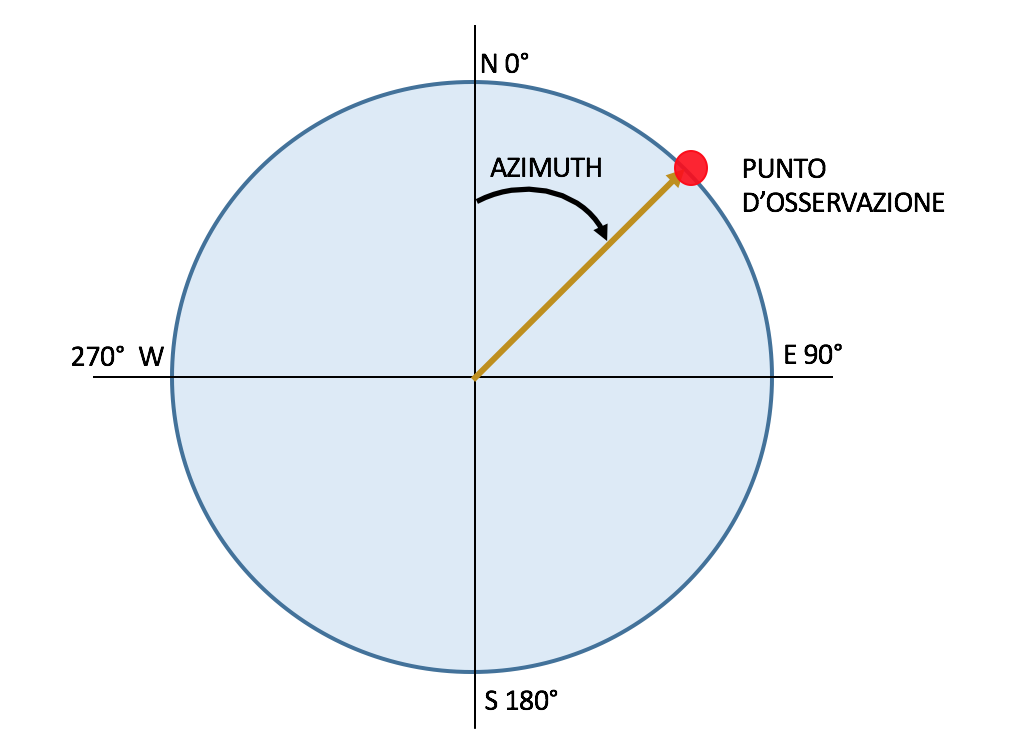
\includegraphics[width=0.6\textwidth]{img/azimuth}
      \caption{Esempio di angolo azimuth per un certo punto}
       \label{fig:azimuth}
\end{figure}



\item \textit{vettoreDirezionale}: il vettore direzionale viene così costruito:
	\begin{enumerate}
	\item trova l'\textit{Azimuth} tra $b_i$ e il punto più vicino della $p_m$ più vicina.
    \item Crea il punto $A$, le cui coordinate $(x_a,y_x)$ sono le coordinate di $b_i$ traslate di $\Delta{x}$ e $\Delta{y}$. \newline
    Dove:
    	\begin{itemize}
    		\item $\Delta{x}= cos (Azimuth) \times (r+1)$
            \item $\Delta{y}= sin (Azimuth) \times (r+1)$
    	\end{itemize}
    con $r$ pari al raggio del $buffer_i$.
    \item crea infine il \textit{vettoreDirezionale}, ovvero il vettore avente come origine $b_i$ e come punto finale il punto $A$ sopra definito.
	\end{enumerate}
    Si propone un esempio esplicativo in Fig.\ref{fig:vettore}.
  \begin{figure}[bth]
  \centering
    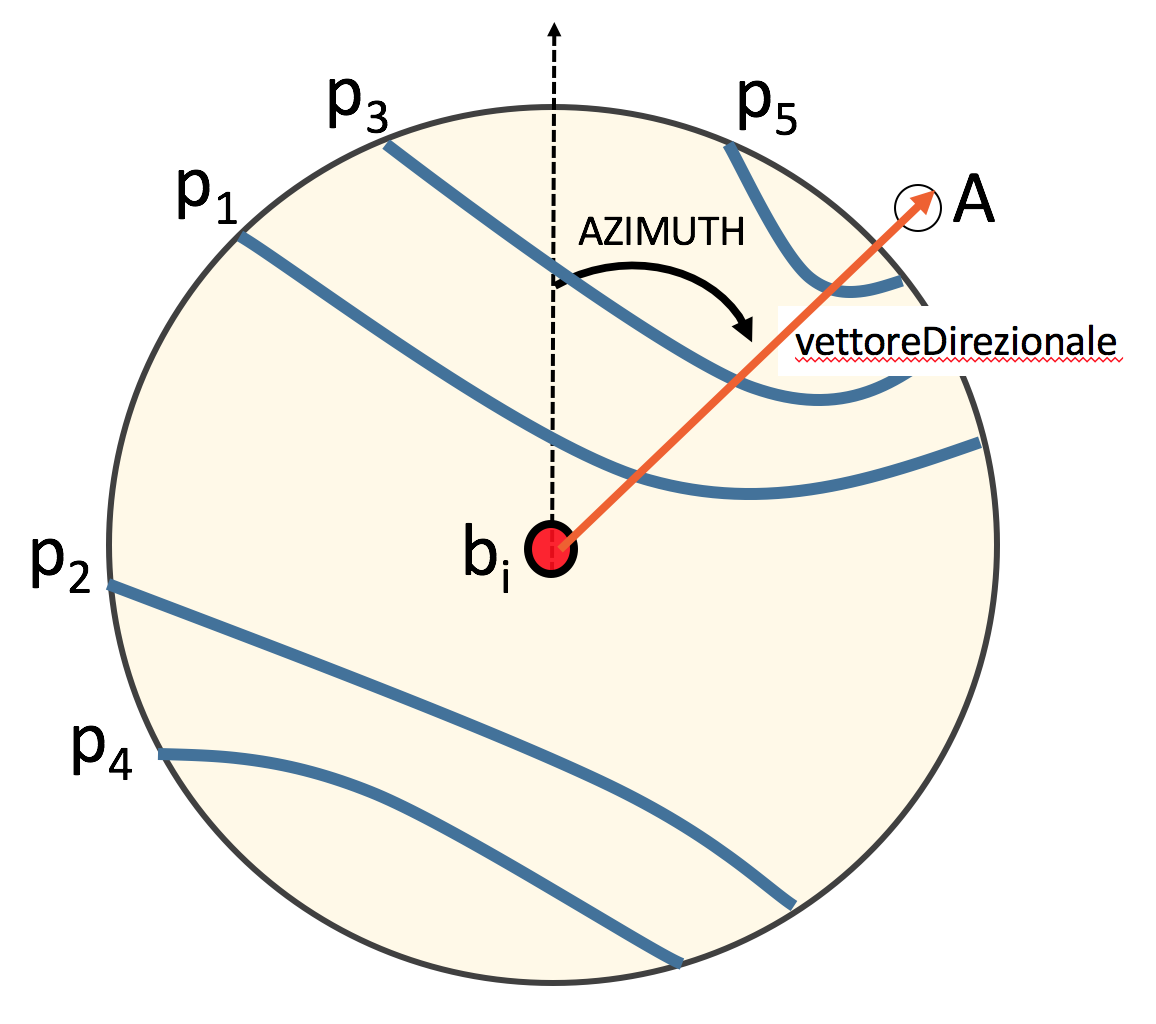
\includegraphics[width=0.5\textwidth]{img/vettore}
      \caption{Esempio di vettore direzionale per un certo edificio $b_i$}
        \label{fig:vettore}

\end{figure}
\newpage
\item \textit{Q}=$\{$ $q_w$ (w=1,2,...,$\beta$)) :=  $p_m$ $\in$ $P$ | $(p_m \cap vettoreDirezionale) \neq \emptyset$ | $d_1$<$d_2$<...<$d_\beta$ $\}$.
\newline
Dove:
\begin{itemize}
\item $d_w$ è la distanza tra $b_i$ e il punto ($p_m \cap vettoreDirezionale$) 
\end{itemize}
Per costruzione i pedici stabiliscono un ordinamento crescente degli elementi dell'insieme $Q$ rispetto la distanza appena definita.\newline
La Fig.\ref{fig:Q} propone un esempio esplicativo basato sulla Fig.\ref{fig:vettore}. Come si vede sono state escluse dall'insieme $Q$ le $p_m$ |($p_m \cap vettoreDirezionale = \emptyset$)  


\begin{figure}[bth]
  
  \centering
    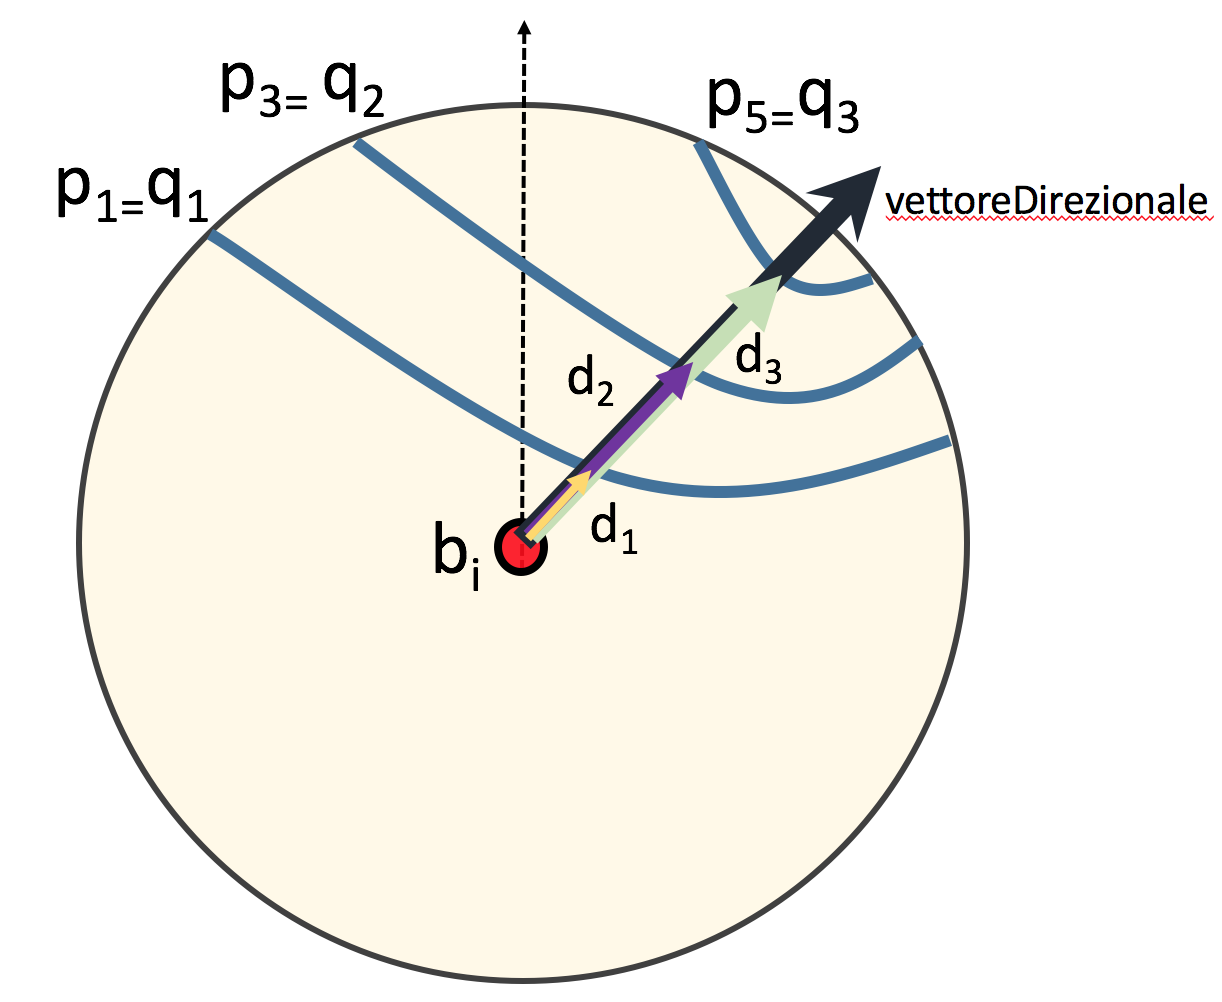
\includegraphics[width=0.5\textwidth]{img/Q}
      \caption{$Q=\{q_1,q_2,q_3\}$}
      \label{fig:Q}
\end{figure}
\newpage

\item \textit{trend}:Il trend rappresenta l'andamento del territorio nelle immediate vicinanze di $b_i$ in direzione del \textit{vettoreDirezionale}  e può assumere uno dei seguenti valori \{\textit{salita}, \textit{discesa}\}, in base alle seguenti condizioni:
\begin{itemize}
\item \textit{trend} = \textit{salita} se $elevation\_q_1 > h\_stazione$.\newline Esempio in Fig.\ref{fig:salita1}

\begin{figure}[bth]
  \centering
    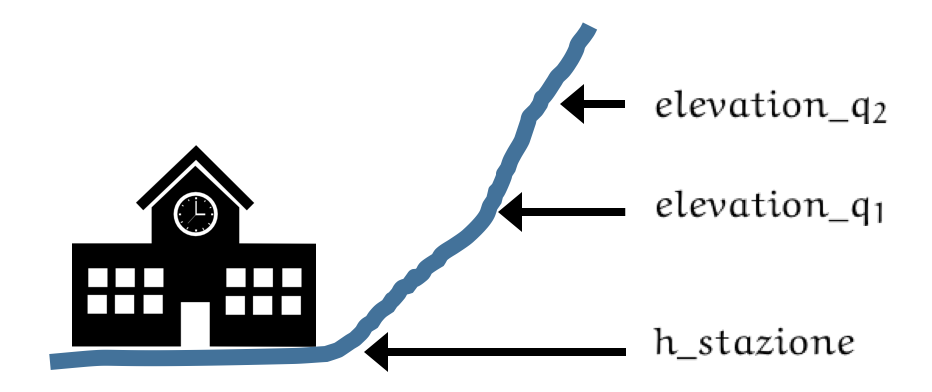
\includegraphics[width=0.8\textwidth]{img/salita1}
      \caption{Esempio di un \textit{trend}=\textit{salita} 
        \label{fig:salita1}
      nel caso in cui la stazione si trova ad una quota minore rispetto la curva di livello $q_1$}
\end{figure}

\item \textit{trend} = \textit{salita} se $elevation\_q_1 = h\_stazione$ $\wedge$ $elevation\_q_2 > elevation\_q_1$. \newline 
Esempio in Fig.\ref{fig:salita2}.
\begin{figure}[bth]
  \centering
    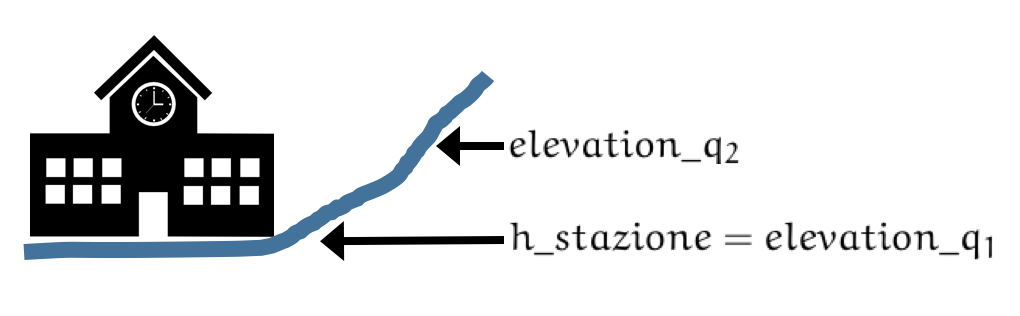
\includegraphics[width=0.8\textwidth]{img/salita2}
      \caption{Esempio di un \textit{trend} = \textit{salita}
        \label{fig:salita2}
nel caso in cui la stazione si trova alla stessa quota della curva di livello $q_1$}
\end{figure}
\newpage

\item \textit{trend} = \textit{discesa} se $elevation\_q_1 < h\_stazione$.\newline
Esempio in Fig.\ref{fig:discesa1}

\begin{figure}[bth]
  \centering
    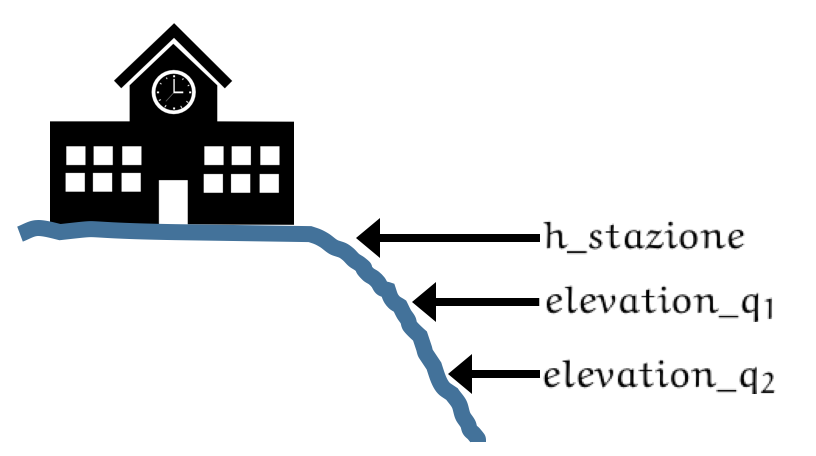
\includegraphics[width=0.8\textwidth]{img/discesa1}
      \caption{Esempio di un \textit{trend}=\textit{discesa}
      \label{fig:discesa1}
nel caso in cui la stazione si trova a quota maggiore rispetto la della curva di livello $q_1$}
\end{figure}



\item \textit{trend} = \textit{discesa} se $elevation\_q_1 = h\_stazione$ $\wedge$ $elevation\_q_2 < elevation\_q_1$.\newline
Esempio in Fig.\ref{fig:discesa2}
\begin{figure}[bth]
  \centering
    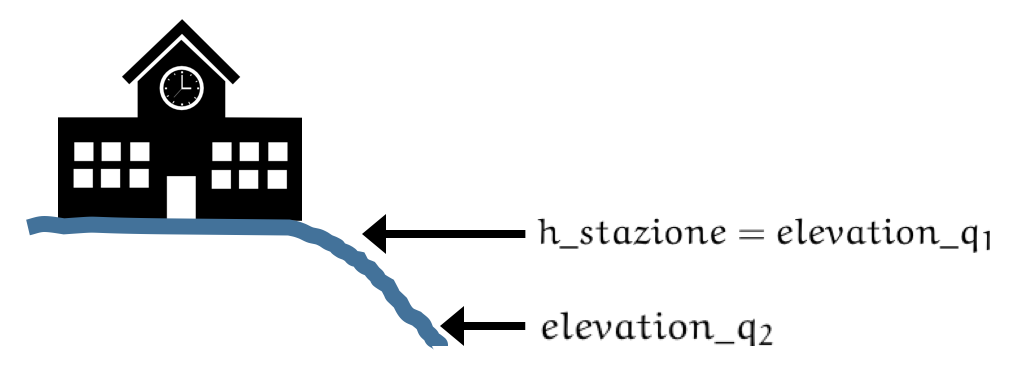
\includegraphics[width=0.8\textwidth]{img/discesa2}
      \caption{Esempio di un \textit{trend}=\textit{discesa}
        \label{fig:discesa2}
nel caso in cui la stazione si trova a quota maggiore rispetto la della curva di livello $q_1$}
\end{figure}

\end{itemize}

\item \textit{situazione Monotonica}: una situazione monotonica è garantita fino ad un certo $q_{\overline{w}}$ se:
\begin{itemize}
\item è garantita $\forall w<\overline{w}$ 
\item la differenza di $elevation$ tra $q_{\overline{w}}$ e $q_{\overline{w}-1}$ conferma l'andamento del \textit{trend}. Ovvero:
\begin{equation}
\label{monotonica}
\begin{cases}
               elevation\_q_{\overline{w}} < elevation\_q_{\overline{w}-1},  & \text{se trend = discesa}\\
               elevation\_q_{\overline{w}} > elevation\_q_{\overline{w}-1}, & \text{se trend = salita}
            \end{cases} 
\end{equation}
\end{itemize} 


\item \textit{pendenza} è una stima dell'andamento del territorio vicino l'edificio $b_i$ lungo il suo $vettoreDirezionale$ associata a q$_w$. Dal punto di vista geometrico la \textit{pendenza} rappresenta il coefficiente angolare tra due punti. In un caso tra una stazione $b_i$ e il punto ottenuto dall'intersezione tra il \textit{vettoreDirezionale} e la curva di livello $q_1$. Nell'altro caso tra i punti ottenuti dall'intersezione tra il \textit{vettoreDirezionale} e le curve $q_w$ e $q_{w+1}$. In entrambi i casi il coefficiente viene calcolato rispetto al sistema di riferimento della \textit{GeoArea}.
Come mostrato nella figura  \ref{fig:pendenza}

\begin{figure}[bth]
\myfloatalign
\subfloat[ ]
{\label{pendenza1}
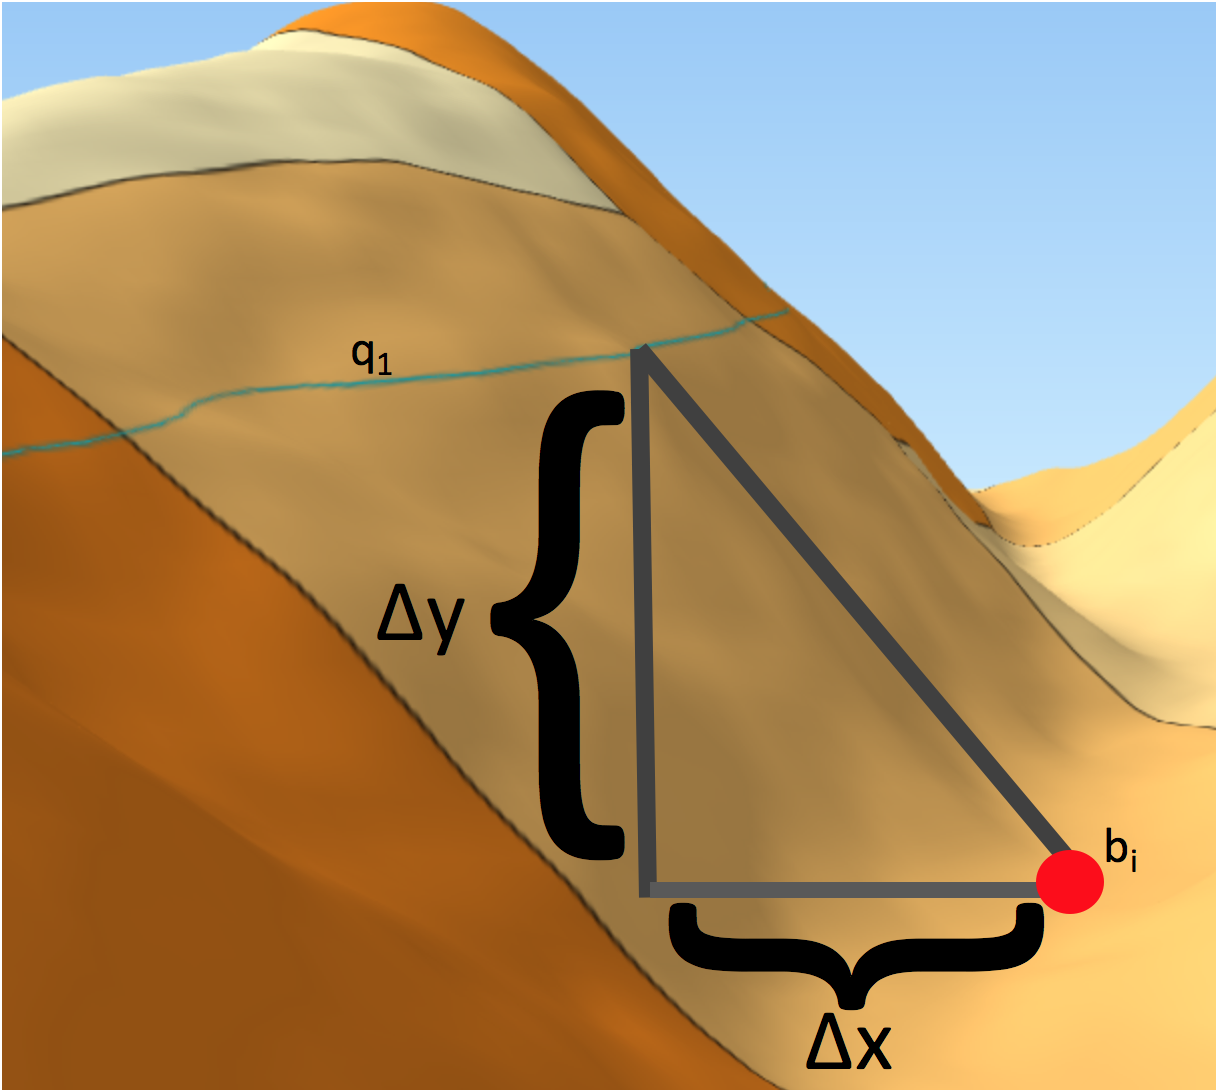
\includegraphics[width=.45\linewidth]{img/pendenza1}} \quad
\subfloat[]
{\label{pendenza2}
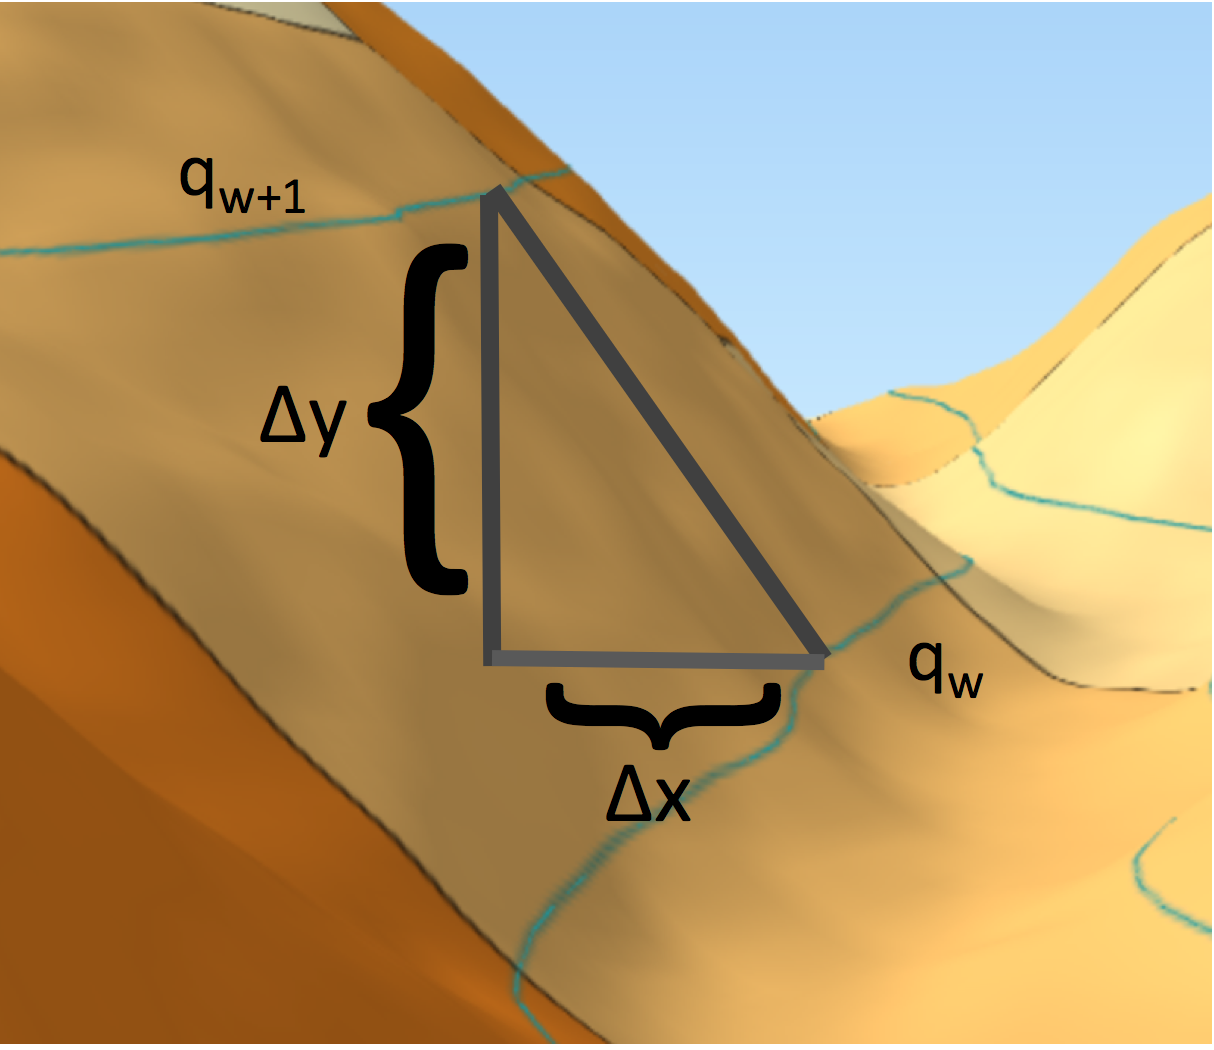
\includegraphics[width=.45\linewidth]{img/pendenza2}} 
\caption[dove]{Esempio esplicativo di \textit{pendenza}.  $\Delta$y corrisponde al numeratore  e $\Delta$x al denominatore dell'Eq.\ref{pendenza}, per $w=1$ subFig.\ref{fig:pendenza} (a) e per w$\geq$2 subFig.\ref{fig:pendenza} (b)}\label{fig:pendenza}
\end{figure}

Dal punto di vista matematico l'equazione per determinare la \textit{pendenza} è la seguente:
\begin{equation}
\label{pendenza}
\begin{cases}
     \frac{| h\_stazione - elevation\_q_w|}
     {d(b_1,(vettoreDirezionale \cap q_w))}  & \text{se w=1}\\
                \frac{| elevation\_q_w - elevation\_q_{w-1}|}
    {d((vettoreDirezionale \cap q_w),(vettoreDirezionale \cap q_{w-1}))} & \text{se w $\geq$ 2}
            \end{cases} 
\end{equation}


\item $slope_i$: E' la somma aritmetica delle \textit{pendenze} di tutti gli elementi di $Q$ che garantiscono una \textit{situazione Monotonica}.

%\item $\alpha_{slope}$: è un fattore moltiplicativo numerico intero, fissato ad un certo valore sulla base di prove sperimentali. Ha lo scopo di eliminare alcuni falsi positivi/negativi.



\end{enumerate}
 

%----------------------------------------------------------------------------------------

\section{Un metodo per classificare le stazioni ferroviarie}


\subsection{Metodo di calcolo originario}
\label{metodoVecchio}
Prima di procedere con l'ideazione di un metodo di calcolo, si è pensato di effettuare un'analisi critica e dettagliata del metodo originario, frutto del lavoro di altri studenti negli anni passati.
Supponiamo di avere quindi una \textit{GeoArea} partizionata in zone diverse e indicate con $z_k$, ognuna delle quali ha associato un valore $s_{zk}$ rappresentante il pericolo di frana. Si ricorda che tali notazioni sono già state introdotte in \ref{notazioni}.
Tale metodo assegna un valore di \textit{exposure} ($Exp_{bi}$) ad un generico edificio ($b_i$) all'interno della \textit{GeoArea} nel seguente modo:
\begin{enumerate}

\item L'\textit{Explosure} per l'edificio $b_i$ è ottenuto come somma dei contributi di tutte le zone nella \textit{Geoarea} per tale edificio.
\begin{equation}
\label{sum_exp_old}
 Exp$\_$b_i = \sum\limits_{k=1}^{\overline{N}}  Exp$\_$b_{i,k}
\end{equation}

\item Il contributo della generica zona $z_k$ all'\textit{exposure} dell'edificio $b_i$ viene calcolato utilizzando la seguente equazione:\newline
\begin{equation}
\label{equazioneVecchia}
Exp$\_$b_i,k = \overline{Size} \times S_{z_k} \times  \begin{cases}
               1,  & \text{se $b_i$ è contenuta in $z_k$}\\
               \frac{1}{d^3}, & \text{altrimenti}
            \end{cases} 
\end{equation}

Dove:
\begin{itemize}
\item \textit{$\overline{Size}$} è il rapporto tra l'area di $z_k$ e l'area media di tutte le zone che costituiscono $Z$
\item \textit{d} denota la distanza minima tra $b_i$ e il \textit{boundary} della zona $z_k$
\end{itemize}
Al prodotto di questi due parametri viene poi moltiplicato un certo valore in base alla posizione relativa tra la zona $z_k$ e l'edificio $b_i$. Tale valore corrisponderà ad 1 se vi è una situazione analoga alla figura seguente:

\begin{figure}[bth]
  \label{fig:stazDentro}
  \centering
    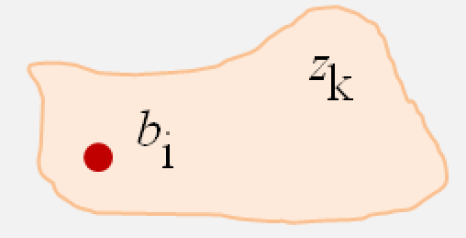
\includegraphics[width=0.5\textwidth]{img/stazDentro}
      \caption{Esempio di un edificio $b_i$ all'interno di una zona                    $z_k$}
\end{figure}

Se invece l'edificio $b_i$ si trova esternamente rispetto alla zona $z_k$, il valore sarà $\frac{1}{d^3}$.

\begin{figure}[bth]
  \label{fig:stazDentro}
  \centering
    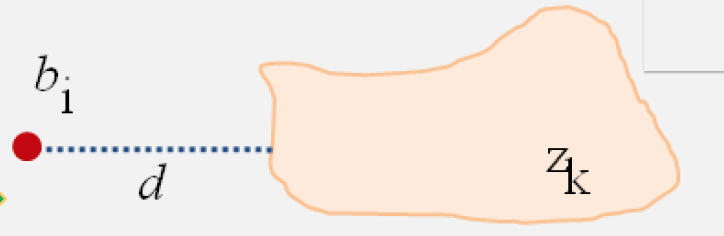
\includegraphics[width=0.5\textwidth]{img/stazFuori}
      \caption{Esempio di un edificio $b_i$ esterno alla zona                    $z_k$}
\end{figure}
\end{enumerate}

Detto ciò possiamo concludere questa breve panoramica sul metodo di calcolo originario con alcune critiche e considerazioni, che hanno rappresentato la base per la realizzazione di un nuovo metodo:
\begin{itemize}
\label{controMetodoVecchio}
\item Il metodo non tiene conto delle curve di livello che cadono nella \textit{GeoArea};
\item Il valore del parametro \textit{Size} è vicino allo zero per zone molto piccole, mentre è maggiore di 1 per tutte le zone che hanno area superiore al valore dell’area media delle zone della \textit{GeoArea}. Inoltre \textit{Size} assume valori molto alti per zone con area molto estesa.
\end{itemize}


\subsection{Metodo di calcolo ex novo}
\label{metodoNuovo}
Il metodo proposto vuole sostituirsi a quello precedente, vedi \ref{metodoVecchio}, con lo scopo di migliorare il calcolo dell'\textit{exposure}. Ovvero si vogliono assegnare valori che rappresentino con maggiore fedeltà il pericolo reale di frana per gli edifici. 
Il punto di forza del nuovo metodo, d'ora in avanti indicato con \textit{NMC}, consiste nello sfruttare il "potenziale informativo" aggiuntivo fornito con l'introduzione delle \textbf{curve di livello}. \newline




Viene da sé che un uso "intelligente" di queste curve, permette di ricavare importanti informazioni ai fini del nostro obiettivo, tra le quali:
\begin{itemize}
\item La quota dell'edificio
\item La morfologia del territorio
\end{itemize}
Supponiamo per un attimo di essere riusciti a ricavare queste informazioni e di averle utilizzate in modo corretto, il \textit{NMC} avrebbe così superato la prima debolezza del metodo originario, vedi \ref{controMetodoVecchio}.
Tuttavia rimarrebbero due questioni in sospeso, ovvero:
\begin{enumerate}
\label{domande}
\item Quali zone $z_k$ della \textit{GeoArea} influiscono realmente sul calcolo dell'\textit{exposure} del generico edificio $b_i$?
\item Supposto di aver trovato risposta al punto precedente, in che proporzione tali zone influiscono? tutte allo stesso modo?
\end{enumerate}
Il metodo originario, rispondeva in parte a queste domande ( vedi equazione \ref{equazioneVecchia}). \newline 
Utilizzando il parametro  $( \frac{1}{d^3} )$  si riusciva a rendere nullo il contributo di zone $z_k$ abbastanza lontane, in quanto la funzione al cubo inversa smorza rapidamente, rispondendo così alla prima domanda.\newline 
Per quanto riguarda il secondo punto, si utilizzava il parametro \textit{Size}, questo però porta alla generazione di falsi positivi/negativi nel calcolo dell'\textit{exposure} dell'edificio, come già sottolineato nel paragrafo precedente.\newline
Dunque vediamo come il \textit{NMC} ricava le informazioni dalle curve di livello e come le utilizza nel calcolo delle \textit{exposure} degli edifici $b_i$. 
\newline
L'equazione del \textit{NMC} che determina il valore finale di \textit{exposure} per la generica $b_i$ è la seguente:
\begin{equation}
\label{sum_exp_nuova}
 Exp\_b_i = (\sum\limits_{\gamma=1}^N  Exp_{bi,\gamma}) + (slope_i \times \alpha_{slope})
\end{equation}
Tale valore dipende dalla somma di due addendi. \newline
Il primo addendo rappresenta la sommatoria dei contributi delle zone $v_\gamma$ $\in$ $V$, ovvero la sommatoria degli \textit{Exp$\_$b$_{i,\gamma}$}. Si ricorda che il limite superiore $N$ della sommatoria nell'Eq.\ref{sum_exp_nuova} si riferisce al numero di zone $v_\gamma$ $\in$ $V$, ovvero alla cardinalità dell'insieme \textit{$V$}. \newline \newline
La formula per calcolare il contributo della zona $v_\gamma$ alla determinazione del pericolo di frana dell'edificio $b_i$ è la seguente:
\begin{equation}
\label{equazioneNuova}
Exp$\_$b_{i,\gamma} = Size \times S_{v_\gamma} \times \Delta{h} \times \begin{cases}
               1,  & \text{se $b_i$ è contenuta in $v_\gamma$ }\\
               \frac{1}{d}, & \text{altrimenti}
            \end{cases} 
\end{equation}
Si notino le differenze rispetto l'equazione del metodo originario ( vedi Eq.\ref{sum_exp_old}). \newline
Nella versione proposta dal \textit{NMC} il parametro ($\frac{1}{d}$) non è elevato al cubo. Questo per evitare di smorzare troppo il contributo delle $v_\gamma$ vicine. Il parametro $Size$ è così definito:
\begin{equation}
\label{size}
 Size= \frac{area (buffer_i \cap v_\gamma)}{area(v_\gamma)} 
\end{equation}

Ovvero l’area della geometria restituita dall’intersezione tra il poligono ($v_\gamma$) e il $buffer_i$ che come abbiamo definito nelle notazioni ha raggio $r$ ed è costruito attorno all'edificio $b_i$. Per un dato valore del raggio $r$, il valore del numeratore dell’Eq. \ref{equazioneNuova} cresce se la posizione di $b_i$ si avvicina al centroide della zona che lo contiene (ovvero $v_\gamma$), di conseguenza, in base all’Eq.\ref{sum_exp_nuova}, anche il corrispondente valore
dell’exposure sarà più alto.

\begin{figure}[bth]
  \label{fig:exBuffer}
   \centering
    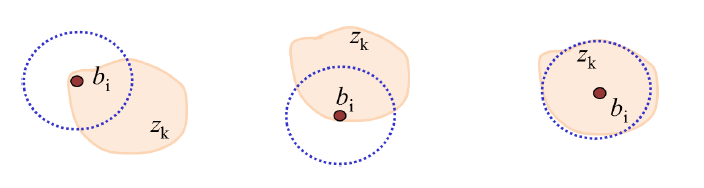
\includegraphics[width=0.8\textwidth]{img/exBuffer}
     \caption{Esempio di un edificio all'interno di una zona $v_\gamma$}
      
\end{figure}
Il parametro \textit{Size} risponde alle domande che ci siamo posti precedentemente (vedi \ref{domande}), ovvero:
\begin{itemize}
\item Quali zone $z_k$ della \textit{GeoArea} influiscono realmente sul calcolo dell'\textit{exposure} di $b_i$? E' facile ora rispondere a questa domanda, tutte e sole le zone $v_\gamma$, ovvero come abbiamo già detto le zone $z_k$ per le quali vale:
\begin{equation}
\label{sizeNotZero}
   area (buffer (b_i,r) \cap z_k) \neq \emptyset
\end{equation}
Bisogna stabilire quanto deve essere il valore del raggio, infatti se tale valore è sufficientemente grande da garantire che eventi franosi a distanza maggiore da $b_i$ non interessino quest'ultimo, allora le zone $z_k$ che non intersecano il $Buffer$ non devono contribuire al calcolo dell'\textit{exposure}. \newline


\item In che proporzione tali zone $v_\gamma$ influiscono? Tutte allo stesso modo? Ovviamente no. Grazie all'espressione \ref{size}, il parametro $Size$ tiene conto anche dell'area effettivamente occupata da $v_\gamma$ all'interno del buffer. In questo modo si riduce notevolmente la probabilità che il \textit{NMC} generi falsi positivi/negativi. \newline 



\end{itemize}


Tale parametro rappresenta, in modo quantitativo, un ulteriore legame tra l'Eq.\ref{equazioneNuova} e la morfologia del territorio. Vediamo un esempio concreto della sua utilità. \newline
La figura \ref{fig:exHmediaAlta} è stata estrapolata mediante il software di visualizzazione di dati territoriali QGIS e mostra una particolare situazione.\newline
La sfera rossa rappresenta un edificio mentre la circonferenza in blu il $buffer$, di cui abbiamo ampiamente parlato, di raggio $r$ pari a $500mt$.

\begin{figure}[bth]
  \centering
  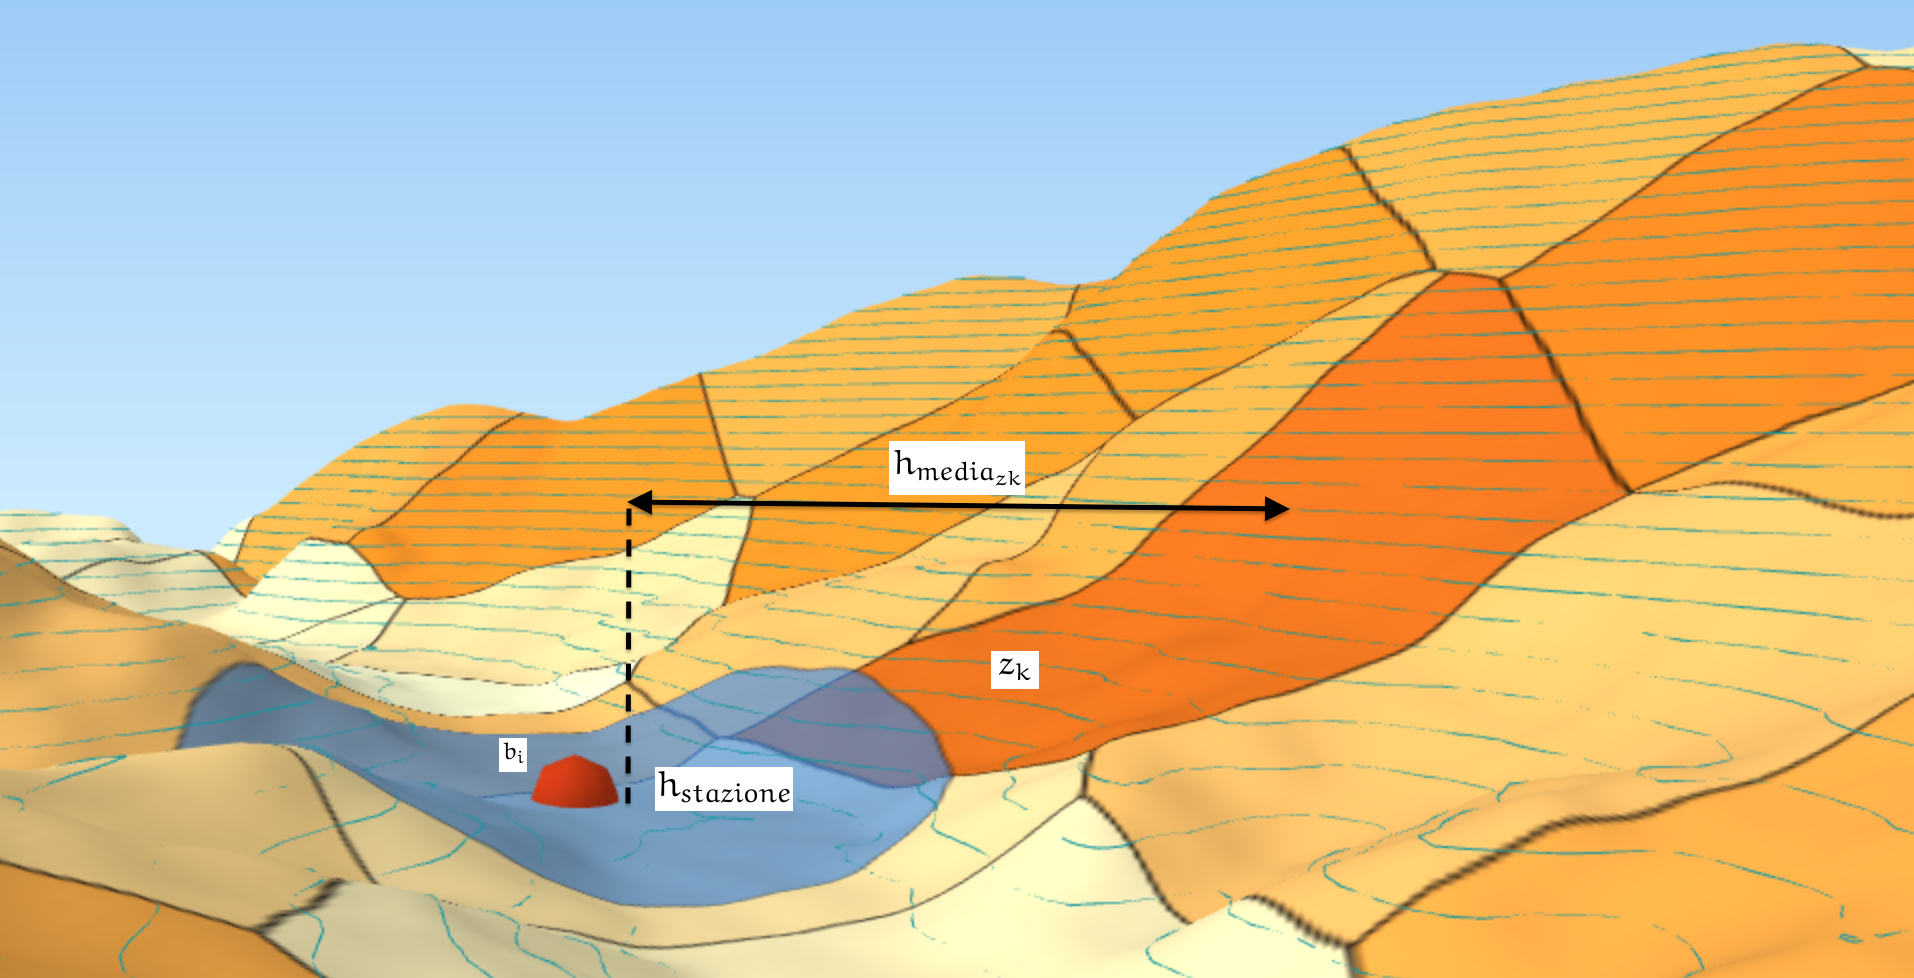
\includegraphics[width=0.8\textwidth]{img/exDeltaH}
  \caption{Esempio di una $v_\gamma$ con $h\_media\_v_{\gamma}$ elevata la cui intersezione con il $buffer_i$ risulta essere un'area piccola } 
  \label{fig:exHmediaAlta}
\end{figure}

Notiamo come la $v_\gamma$ in questione occupi una parte molto piccola del $buffer_i$. Questo sicuramente porterà ad avere un valore di $Size$ molto basso e di conseguenza anche il contributo di $v_\gamma$ all'\textit{exposure}, generando un falso negativo. Il fattore $\Delta{h}$ interviene in soccorso di $Size$, permettendo all' $Exp_{bi,\gamma}$ di assumere in valore non eccessivamente basso, tenendo conto dell'elevata differenza tra l'altezza della stazione $b_i$ e l'altezza media di $v_\gamma$.

Il secondo addendo dell'Eq.\ref{sum_exp_nuova} va a rappresentare un fattore di rischio dovuto al dislivello che si trova più vicino a b$_i$ e che quindi va considerato con maggior peso.\\ 
$\alpha_{slope}$ è un fattore moltiplicativo intero utilizzato per incrementare o diminuire il peso  di $slope_i$ nel calcolo di $Exp\_b_i$ rispetto al primo addendo.\\ 
%Sperimentalmente si osserva che ponendo $\alpha_{slope}$ pari ad 1 il contributo di $slope_i$ viene quasi trascurato mentre ponendolo pari a 10 questo va a sovrastare il contributo del primo addendo. Un valore che rappresenta un buon compromesso tra le precedenti situazioni è $\alpha_{slope}$ = 5.  

 

%----------------------------------------------------------------------------------------

\subsection{L'algoritmo}

Lo scopo di questo paragrafo è formalizzare gli algoritmi che implementa \textit{NMC}, descritto nella sezione 2.2.2 .\\ 
\newline
\newline
\textbf{Algoritmo 1}\\
\newline
Il primo algoritmo denominato $averageElevationNearZones$ ha come obiettivo quello di calcolare il valore di $avgElevation$ associato ai v$_\gamma$ in \textit{V}. Prende come parametri di input gli insiemi \textit{Z}, \textit{E} e l'elemento buffer$_i$ mentre restituisce come output l'insieme \textit{V}.\\

\begin{algorithm}[H]
	
	\SetKwData{Left}{left}\SetKwData{This}{this}\SetKwData{Up}{up}
	\SetKwFunction{Union}{Union}\SetKwFunction{FindCompre
ss}{FindCompress}
	\SetKwInOut{Input}{Input}\SetKwInOut{Output}{Output}

	\IncMargin{1em}
	\Input{\textit{Z}, \textit{E}, buffer$_i$}
	\Output{\textit{V}}
	\KwResult{Calcola la quota media delle zone che intersecano il buffer}
	\caption{averageElevationNearZones}
	\label{alg:one}
	\BlankLine
	
	\SetAlgoNoLine
	\textit{V}=$\emptyset$; \\
    avgElevation = $0$; \\
    contatore = $0$; \\
    
	\For{each z$_k$ $\in$ \textit{Z}}{
    	\If{z$_k$ $\cap$ \textit{buffer$_i$}}{
        	\For{each e$_j$ $\in$ \textit{E}}{
            	\If{z$_k$ $\cap$ e$_j$}{
                $avgElevation$ = $avgElevation$ + ( $elevation$ di e$_j$ ); \\
                $contatore$ = $contatore$ + 1; \\
                }
            }
            \If{contatore > $0$}{
    			$avgElevation$ = $avgElevation$/$contatore$;
    		}
			aggiorna il valore $avgElevation$ di z$_k$;\\
            v$_\gamma$ = z$_k$;\\
    		\textit{V} = \textit{V} $\cup$  v$_\gamma$;\\ 
            avgElevation = $0$; \\
    		contatore = $0$; \\
        }  
    }
	return \textit{V}; 
	

\end{algorithm}

\mbox{}\\
Commenti:\\
Dalla riga 1 alla 3 sono presenti alcune inizializzazioni: l'insieme \textit{V} inizialmente è vuoto, mentre sono fissati a $0$ i valori di $avgElevation$ e $contatore$. Dalla riga 4 alle 21 è presente un ciclo che scandisce gli elementi z$_k$ di \textit{Z}. Immediatamente all'interno del ciclo (righe 5-20) viene effettuato un controllo che verifica se la zona in esame ha un'intersezione con il buffer.\\ 
In caso di esito negativo si passa subito al successivo elemento di \textit{Z}. In caso di esito positivo, per ogni elemento e$_j$ in E, si verifica se interseca con la zona z$_k$ in esame. Se anche questo controllo viene superato si incrementa il valore di $avgElevation$ con l'$elevation$ di e$_j$ e il valore di $contatore$ di 1.\\
Una volta completato il ciclo sugli elementi in \textit{E}, si controlla (riga 12) se $contatore$ ha un valore maggiore di zero, quindi se almeno per una linea e$_j$ è verificata l'intersezione con la z$_k$ esaminata. In questo caso il valore di $avgElevation$ viene sovrascritto a $avgElevation/contatore$.\\
Si passa quindi (riga 15) ad aggiornare il valore $avgElevation$ nella tupla z$_k$ con il valore appena calcolato.\\
Alla riga 16 la tupla z$_k$ viene copiata nella tupla v$_\gamma$ che viene inserita nell'insieme \textit{V}. Questa operazioni viene eseguita per mantenere nell'insieme \textit{V} solo gli elementi z$_k$ di interesse, ossia quelli per cui è verificata l'intersezione con $buffer_i$.\\  
Alle righe 18 e 19 le variabili $avgElevation$ e $contatore$ sono resettate a $0$, per poter essere appropriatamente riutilizzate nella successiva iterazione del ciclo.\\
L'algoritmo infine (riga 22) restituisce l'insieme \textit{V}.\\
\mbox{}\\
Riassumendo l'algoritmo prende tutte e sole le z$_k$ che intersecano il buffer e per ognuna calcola la quota media. Inserisce infine queste zone nell'insieme \textit{V} che restituisce come risultato.\\
La complessità computazionale dell'algoritmo è data dal ciclo in riga 4 e da quello in riga 6. È quindi pari a $\mathcal{O}(card(\textit{Z}) \times card(\textit{E}))$ anche se mediamente è molto inferiore in quanto è molto improbabile che ogni elemento in \textit{Z} intersechi con buffer$_i$ e con tutte le linee in \textit{E}. 
\mbox{}\\
\newline
\newline
\textbf{Algoritmo 2}\\
\newline
L'algoritmo denominato $elevationBuild$ ha come obiettivo quello di stimare l'$elevation$ di b$_i$. Prende come parametri di input gli insiemi \textit{V} (l'insieme delle zone che intersecano buffer$_i$), \textit{E} (l'insieme delle curve di livello) e l'elemento b$_i$. In output restituisce lo stesso elemento b$_i$ di input il cui campo $elevation$ è stato aggiornato con la stima calcolata.\\ 

\begin{algorithm}[H]
	
	\SetKwData{Left}{left}\SetKwData{This}{this}\SetKwData{Up}{up}
	\SetKwFunction{Union}{Union}\SetKwFunction{FindCompre
ss}{FindCompress}
	\SetKwInOut{Input}{Input}\SetKwInOut{Output}{Output}

	\IncMargin{1em}
	\Input{\textit{V}, \textit{E}, b$_i$}
	\Output{\textit{b$_{i}$}}
	\KwResult{Calcola una stima dell'elevation di b$_i$}
	\caption{elevationBuild}
	\label{alg:one}
	\BlankLine
	
	\SetAlgoNoLine
	
    \textit{T}=$\emptyset$; \\
	\For{each v$_{\gamma}$ $\in$ \textit{V}}{
    	\For{each e$_j$ $\in$ \textit{E}}{
        	\If{v$_{\gamma}$ $\cap$ e$_j$}{
            	$geom$ di t$_f$ = st\_intersection ( v$_{\gamma}$, e$_j$ );\\
                $elevation$ di t$_f$ = $elevation$ di e$_j$; \\
            	\textit{T}=\textit{T} $\cup$ t$_f$;
            }
    	}
    }
    \For{each t$_f$ $\in$ \textit{T}}{
    	$dist$ = st\_distance ( b$_i$, t$_f$ );\\
        Trova t$_{fmin}$  t.c. $dist$ è minima;\\
        Trova t$_{fmin2}$   t.c. $dist$ è la successiva al minimo; \\
    }
    \If{b$_i$ in posizione atipica}{
		t$_{fmin2}$ = t$_{fmin}$;\\
    }
    Calcola $h\_stazione$ \\
    Aggiorna $elevation$ di b$_i$ con $h\_stazione$;\\
	return b$_{i}$; \\
	

\end{algorithm}

\mbox{}\\
Commenti:\\
Nella prima riga dell'algoritmo l'insieme \textit{T} è inizializzato come insieme vuoto.\\ 
Nelle righe 2-10 è presente un ciclo annidato. Il ciclo più esterno itera sugli elementi v$_\gamma$ in \textit{V} (l'insieme delle zone che intersecano il buffer), mentre quello più interno sugli elementi e$_j$ in \textit{E} (l'insieme delle linee di livello). Se l'intersezione tra gli elementi v$_\gamma$ e e$_j$ esiste, allora questa intersezione viene assegnata come geometria di t$_f$ mentre come sua $elevation$ viene assegnata l'elevation di e$_j$. L'ennupla t$_f$ così definita è inserita nell'insieme \textit{T} (riga 7). \\
All'interno del ciclo in riga 11 si vanno a scandire i t$_f$ in \textit{T}. All'interno del ciclo si va a calcolare la distanza $dist$ tra l'elemento t$_f$ e b$_i$. Si vanno quindi a individuare (nelle righe 13-14) t$_{fmin}$ e t$_{fmin2}$.\\
t$_{fmin}$ è la t$_f$ $\in$ \textit{T} tale che la distanza $dist$ tra  t$_f$ e b$_i$ è la distanza minima tra tutte le distanze calcolate tra ogni altra t$_f$ $\in$ \textit{T} e b$_i$.\\
In modo analogo t$_{fmin2}$ è la t$_f$ $\in$ \textit{T} la cui distanza $dist$ tra  t$_f$ e b$_i$ ha un valore immediatamente successivo alla distanza minima.\\
Alla riga 16 si effettua un controllo per verificare se b$_i$ si trova in una posizione "atipica" come definito nella sezione 2.1. Nel caso di esito positivo si copia l'ennupla t$_{fmin}$ in t$_{fmin2}$.\\
Si calcola quindi alla riga 19 il valore di $h\_stazione$ come descritto precedentemente (in sezione 2.1), dove t$_fmin$ rappresenta da e$_1$, mentre t$_{fmin2}$ rappresenta e$_2$.\\
Nella riga 20 si aggiorna l'$elevation$ di b$_i$ con il valore appena calcolato $h\_stazione$. Viene infine restituiti b$_i$.\\
\mbox{}\\
Riassumendo l'algoritmo individua i segmenti di linea frutto dall'intersezione tra tutte le linee in \textit{E} e le zone in \textit{V} e li inserisce nell'insieme \textit{T}. Individua poi i 2 elementi in \textit{T} che sono più vicini a b$_i$. Sfruttando questi 2 elementi calcola $h\_stazione$ cioè una stima dell'elevation di b$_i$.\\
La complessità computazionale è data dal ciclo annidato in riga 2 ed è pari a $\mathcal{O}(card(\textit{V}) \times card(\textit{E}))$ anche se mediamente è molto inferiore in quanto è molto improbabile che ogni elemento in \textit{V} intersechi tutte le linee in \textit{E}.\\ 
\mbox{}\\
\newpage
\textbf{Algoritmo 3}\\
\newline
L'algoritmo denominato $slopeFactor$ ha come obiettivo quello di calcolare lo $slope$ associato a b$_i$. Prende come parametri di input l'insieme \textit{E} delle curve livello e l'elemento buffer$_i$, mentre restituisce $slope_i$ ossia lo slope associato a b$_i$.\\ 

\begin{algorithm}[H]
	
	\SetKwData{Left}{left}\SetKwData{This}{this}\SetKwData{Up}{up}
	\SetKwFunction{Union}{Union}\SetKwFunction{FindCompre
ss}{FindCompress}
	\SetKwInOut{Input}{Input}\SetKwInOut{Output}{Output}

	\IncMargin{1em}
	\Input{\textit{E}, buffer$_i$}
	\Output{\textit{slope$_{i}$}}
	\KwResult{Calcola lo $slope$ associato a b$_i$}
	\caption{slopeFactor}
	\label{alg:one}
	\BlankLine
	
	\SetAlgoNoLine
	
    \textit{P}=$\emptyset$; \\
    \textit{Q}=$\emptyset$; \\
    slope$_i$ = $0$;\\
    \For{each e$_j$ $\in$ \textit{E}}{
    	\If{buffer$_i$ $\cap$ e$_j$}{
        	$geom$ di p$_m$ = st\_intersection ( buffer$_i$, e$_j$ );\\
            $elevation$ di p$_m$ = elevation di e$_j$;\\
            \textit{P} = \textit{P} $\cup$ p$_m$;\\
        }
    }
    Calcola il $vettoreDirezionale$;\\
    \For{each p$_m$ $\in$ \textit{P}}{
    	\If{p$_m$ $\cap$ $vettoreDirezionale$}{
        	Calcola la distanza tra b$_i$  e (p$_m$ $\cap$ $vettoreDirezionale$);\\
        	Aggiorna $distance$ di p$_m$ con la distanza calcolata;\\
            q$_w$ = p$_m$;\\
            Q = Q $\cup$ q$_w$ ;\\
        }
    }
    \For{each q$_w$ $\in$ \textit{Q} ordinato rispetto a $distance$}{
		slope$_i$ = slope$_i$ + (pendenza associata a q$_w$);
    }

	return slope$_{i}$; \\
	

\end{algorithm}
\mbox{}\\
Commenti:\\
Nelle prime righe (1-3) vengono inizializzati gli insiemi \textit{P}, \textit{Q} come insiemi vuoti e la variabile $slope_i$ a zero.\\
Dalla riga 4 inizia un ciclo che scandisce gli elementi e$_j$ in \textit{E} e per ognuno controlla se interseca con buffer$_i$. Se questa intersezione esiste, questa viene assegnata come geometria di p$_m$ mentre come sua $elevation$ viene assegnata l'$elevation$ di e$_j$. La tupla p$_m$ così definita, viene inserita nell'insieme \textit{P}. Queste operazioni permettono di lavorare su un insieme che è molto più piccolo di \textit{E} e che contiene solo le porzioni di linee di interesse.\\
Alla riga 11 viene calcolato il $vettoreDirezionale$ come definito nella sezione 2.1.\\
Nella righe 12-19 è presente un ciclo che scandisce gli elementi p$_m$ in \textit{P} e per ognuno verifica se interseca con il $vettoreDirezionale$. Se questa intersezione esiste viene calcolata la distanza tra b$_i$ e l'intersezione. Il valore di distanza calcolato va ad aggiornare il valore $distance$ in p$_m$. La tupla p$_m$  così costruita viene quindi copiata in q$_w$. Alla riga 17, q$_w$ viene inserito nell'insieme  \textit{Q}. In questo modo in \textit{Q} si vanno a inserire tutti e soli gli elementi p$_m$ che intersecano il $vettoreDirezionale$. \\
Nella riga 20 inizia un ciclo che scandisce gli elementi q$_w$ in \textit{Q} ordinati rispetto al campo $distance$. All'interno del ciclo viene calcolata la pendenza associata a q$_w$ come definita nelle sezione 2.1. Questo valore va a incrementare slope$_i$.\\ 
Viene infine restituito slope$_i$.\\
\mbox{}\\
Riassumendo l'algoritmo individua le porzioni di linee di livello che si trovano tutte in una stessa direzione rispetto a b$_i$ e per ognuna di esse calcola la pendenza, ossia la ripidità tra la linea e la linea precedente, dove la linea precedente è più vicina a b$_i$. slope$_i$ è la somma di queste pendenze.\\
La complessità computazionale è data dal ciclo in riga 4 ed è quindi pari a $\mathcal{O}(card(\textit{E}))$.\\
\mbox{}\\
\newpage
\textbf{Algoritmo 4}\\
\newline
L'algoritmo denominato $computeExplosure$ è l'algoritmo che effettivamente calcola l'$explosure$ associato a b$_i$. All'interno dell'algoritmo vengono richiamati tutti e tre gli algoritmi precedentemente definiti.\\

\begin{algorithm}[H]
	
	\SetKwData{Left}{left}\SetKwData{This}{this}\SetKwData{Up}{up}
	\SetKwFunction{Union}{Union}\SetKwFunction{FindCompre
ss}{FindCompress}
	\SetKwInOut{Input}{Input}\SetKwInOut{Output}{Output}

	\IncMargin{1em}
	\Input{\textit{B}, $r$, $\alpha_{slope}$, \textit{E}, \textit{Z}}
	\Output{\textit{B}}
	\KwResult{Calcola l'$explosure$ di tutte le  b$_i$}
	\caption{computeExplosure}
	\label{alg:one}
	\BlankLine
	
	\SetAlgoNoLine
	
    \For{each b$_i$ $\in$ \textit{B}}{
    	buffer$_i$ = st\_buffer( b$_i$, $r$ );\\
        \textit{V} = averageElevationNearZones ( \textit{Z}, \textit{E}, buffer$_i$ );\\
        b$_i$ =  elevationBuild ( \textit{V}, \textit{E}, b$_i$ );\\
        slope$_i$ = slopeFactor ( \textit{E}, b$_i$, buffer$_i$);\\
        \For{each v$_\gamma$ $\in$ \textit{V}}{
        	Calcola $Size$;\\
            Calcola $Exp\_b_{i,\gamma}$;\\
        }
        Calcola $Exp\_b_i$;\\
        Aggiorna il valore di $Exp\_b_i$ in b$_i$;\\
    }


	return \textit{B}; \\
	

\end{algorithm}
\mbox{}\\
Commenti:\\
Nelle righe 1-11 è presente un ciclo che scandisce tutte le b$_i$ in B.
Per ogni b$_i$ viene calcolato un buffer circolare di raggio $r$.  Viene successivamente costruito un insieme \textit{V}  che contiene tutte le zone che intersecano il buffer, dove a ogni zona viene associata una quota media (richiamando l'algoritmo 1).\\ 
Nella riga 4 la tupla b$_i$ viene aggiornata inserendo un valore che rappresenta una stima della sua quota (richiamando l'algoritmo 2).\\
Nella riga 5 viene quindi calcolato slope$_i$ (richiamando l'algoritmo 3).\\
Dalla riga 6 inizia un ciclo che scandisce gli elementi in \textit{V} e per ognuno calcola $Size$ e Exp\_b$_{i,\gamma}$.\\
In riga 10 si calcola $Exp\_b_i$ (tenendo conto anche del fattore $\alpha_{slope}$ come mostrato nell'Eq.\ref{sum_exp_nuova}) che va ad aggiornare il valore nella tupla b$_i$.\\
L'algoritmo ritorna come risultato l'insieme \textit{B} dove ogni tupla b$_i$ viene arricchita con un stima della quota e un valore di $Explosure$. 
\mbox{}\\
La complessità computazionale è data dai due cicli presenti alle righe 1 e 10 ed è quindi pari a $\mathcal{O}(card(\textit{V}) \times card(\textit{B}))$. \\
\mbox{}\\





\section{Un metodo per classificare le linee ferroviarie}
Il metodo proposto per classificare le stazioni (vedi Sez.\ref{metodoNuovo}) può essere utilizzato anche per classificare le linee ferroviarie. Occorre tuttavia estendere il NMC a causa della diversa rappresentazione geometrica dei due elementi.


\subsection{Metodo di calcolo}
\label{metodoLinee}
Poiché il NMC è stato progettato per classificare stazioni,  rappresentate attraverso dei punti geometrici, non può essere utilizzato così com'è per classificare le linee ferroviarie rappresentate invece attraverso linee geometriche (Fig.\ref{lineeFerroviarie}).

\begin{figure}[bth]
  \centering
  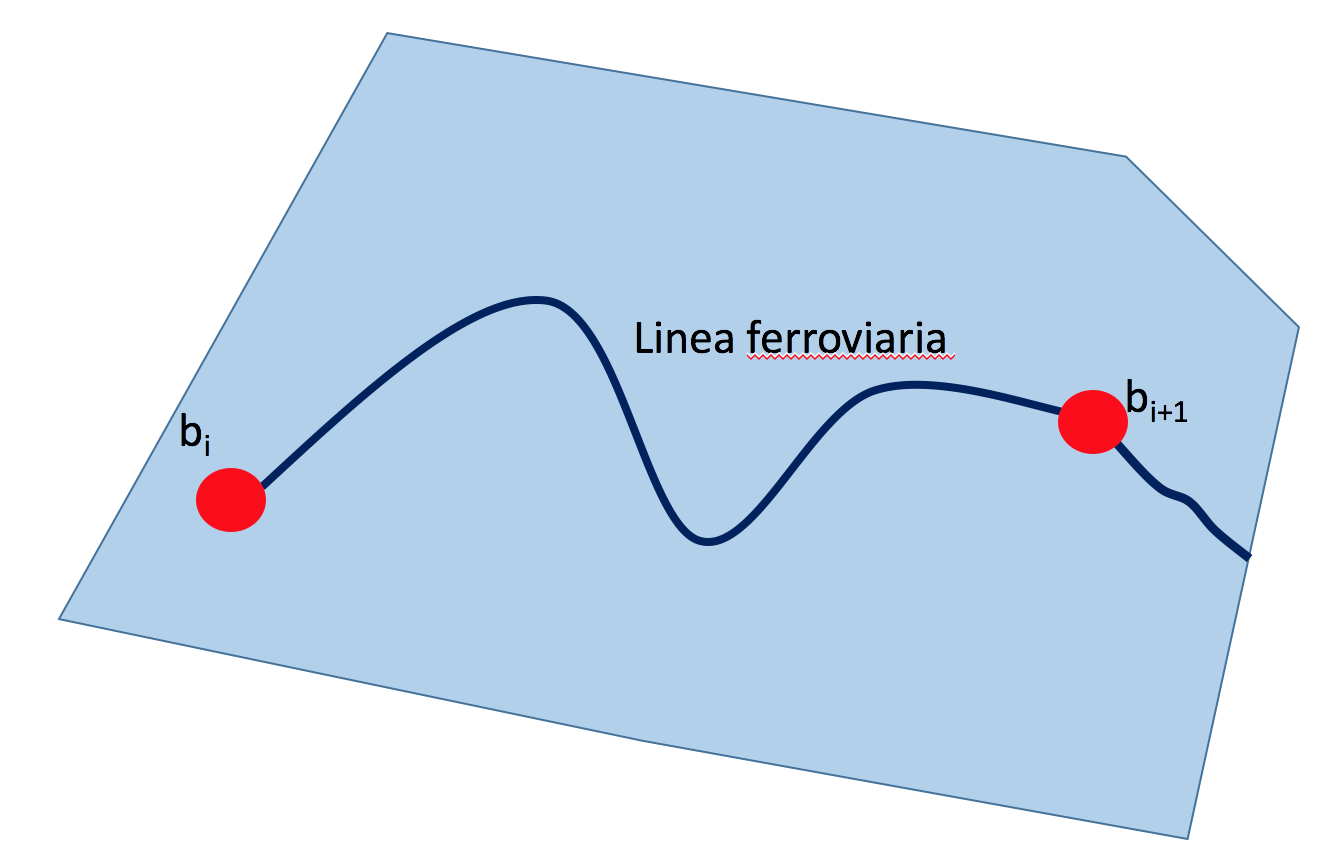
\includegraphics[width=0.7\textwidth]{img/lineaFerroviaria}
  \caption{Esempio di rappresentazione geometrica di una linea ferroviaria ove $b_i$ e $b_{i+1}$ sono due stazioni } 
  \label{lineeFerroviarie}
\end{figure}
L'idea di fondo è campionare con un certo passo, le linee ferroviarie. Fatto ciò si avrà una sequenza di punti sui quali poter applicare il NMC. \newline
Nonostante l'idea sembri essere molto semplice, ci sono tre questioni sulle quali bisogna fare delle riflessioni e proporre delle soluzioni:
\begin{enumerate}
\item che passo di campionamento adottare? La scelta di un passo piccolo giova alla correttezza del calcolo finale di \textit{exposure} della tratta ma aumenta significativamente i tempi di esecuzione del calcolo stesso.
\item le linee sono semplici? Le linee ferroviarie potrebbero avere delle traiettorie complesse, il metodo deve essere in grado di gestirle.
\item come aggregare i punti campionati? Dopo aver campionato una certa tratta e aver determinato i valori di \textit{exposure} di ogni punto della sequenza che la compongono, bisognerà aggregare in qualche modo tali risultati per poter aver un risultato utile e consultabile.  
Il campionamento potrebbe generare un numero considerevole di punti che presi singolarmente non forniscono un contributo significato al problema in questione ( vedi Sez. \ref{ch:introduzione})
\end{enumerate}
L'estensione del NMC (d'ora in avanti indicato con NMCE, dove E sta per esteso) per le linee ferroviarie propone una soluzione per ognuna di queste problematiche. Nell'ordine in cui sono state precendetemente presentate: 
\begin{enumerate}
\item Il passo di campionamento scelto è di 300 mt, ma può essere facilmente modificato essendo un parametro del metodo(Fig.\ref{puntiLinea})
\begin{figure}[bth]
	\centering
	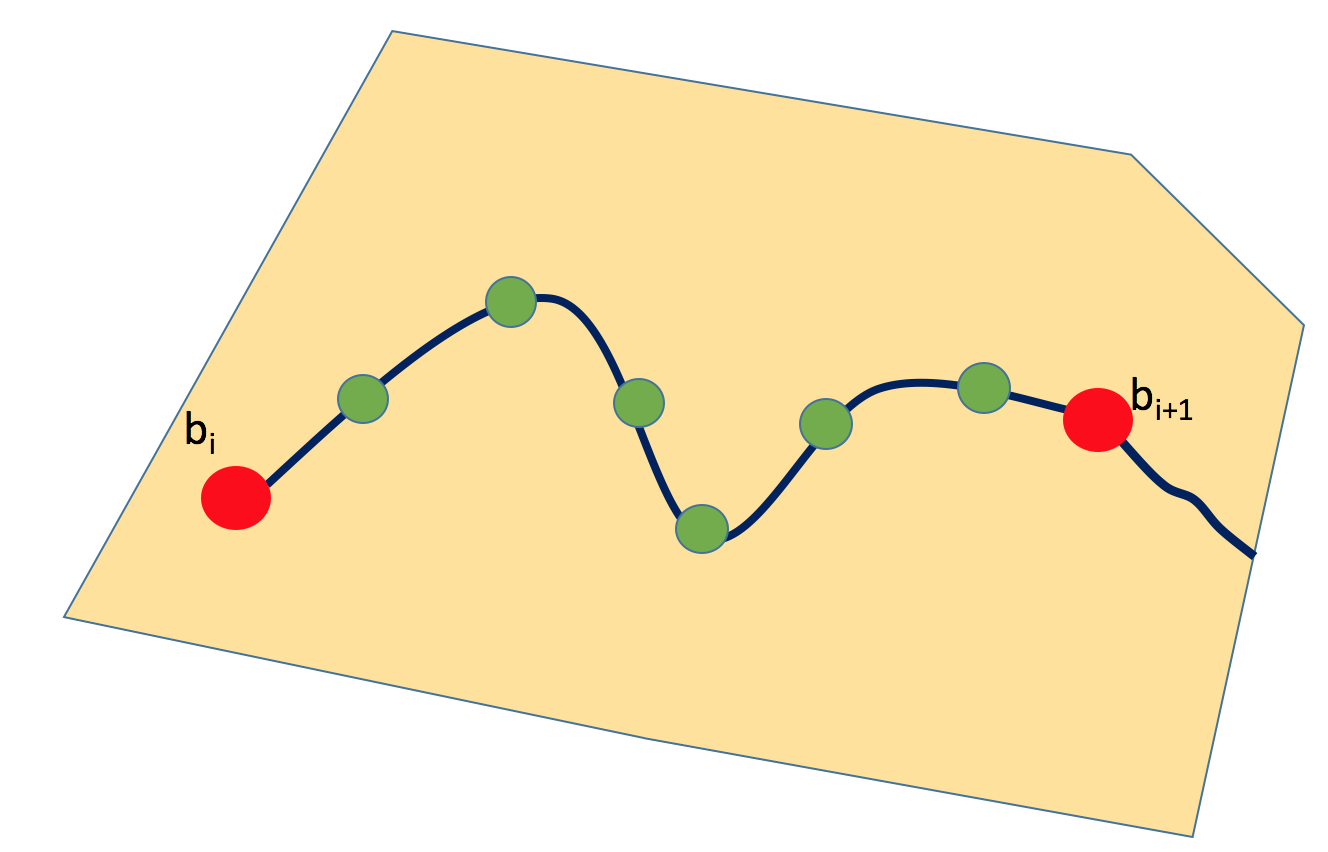
\includegraphics[width=0.5\textwidth]{img/puntiLinea}
	\caption{Esempio di campionamento di una linea ferroviaria } 
	\label{puntiLinea}
\end{figure}

\item nel caso in cui una tratta abbia una traiettoria complessa, il NMCE rileva tale situazione e provvede a dividere la linea in due o più linee semplici. In Fig.\ref{fig:divisioneLinea} un esempio esplicativo.

\begin{figure}[bth]
\myfloatalign
\subfloat[]
{\label{lineaComplessa}
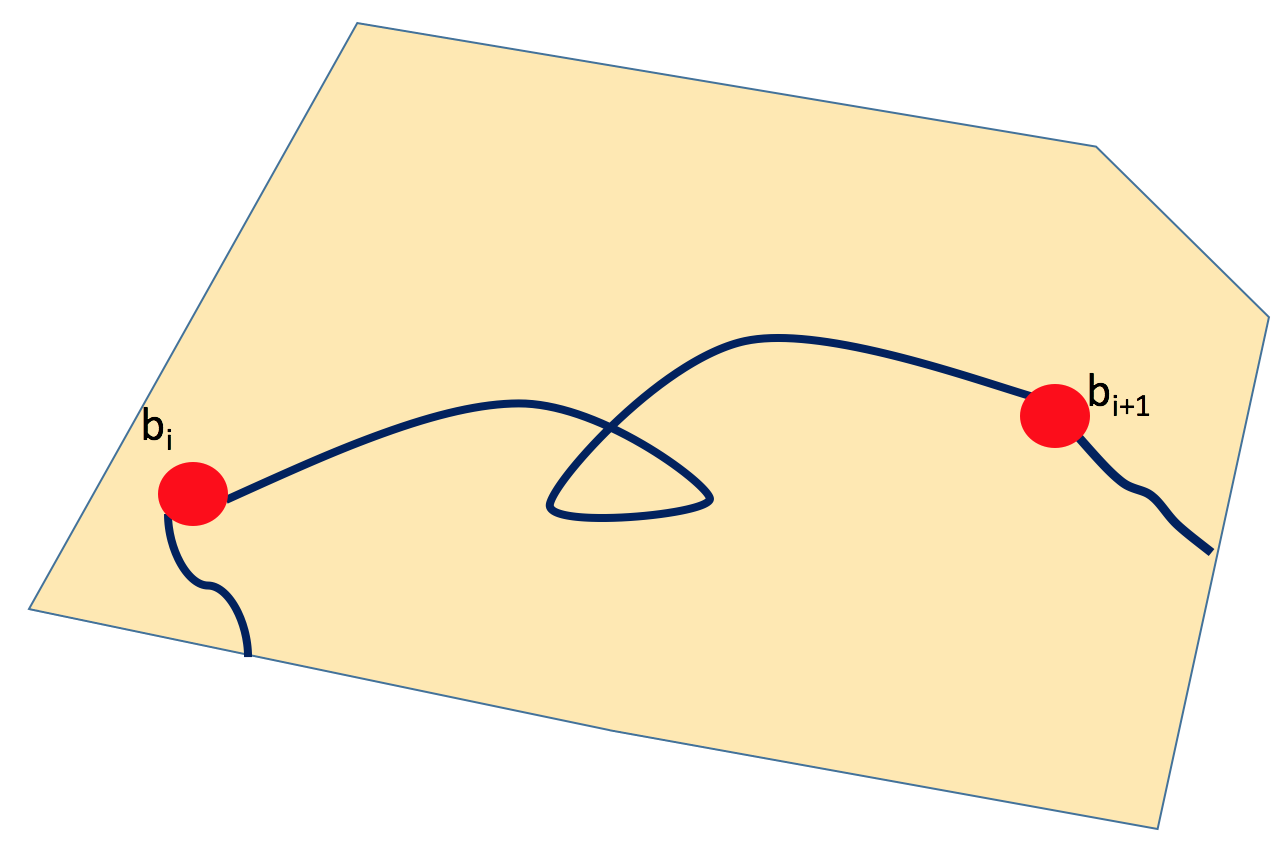
\includegraphics[width=.45\linewidth]{img/lineaComplessa}} \quad
\subfloat[ ]
{\label{lineeSemplici}
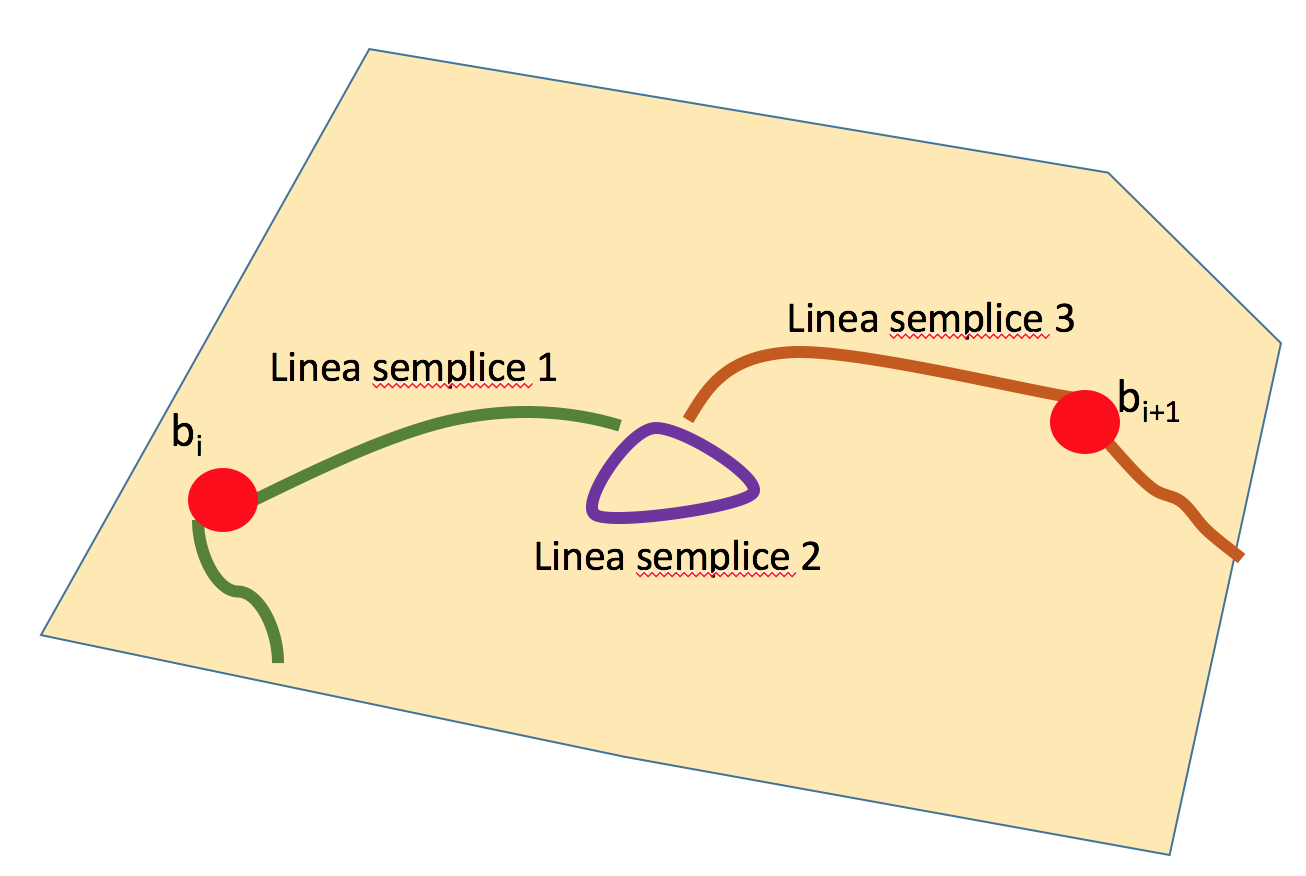
\includegraphics[width=.45\linewidth]{img/lineaSemplice}} 
\caption[dove]{Esempio di una linea complessa (a) e della sua divisione in tre linee semplici (b)}
\label{fig:divisioneLinea}
\end{figure}


\item una volta campionato la tratta semplice, si utilizza il NMC per determinare il valore di \textit{exposure} di ogni punto che la compone. \newline
La linea ferroviaria viene quindi divisa in segmenti di lunghezza arbitraria, nel nostro caso 1 km ciascuno (fatta eccezione per l'ultimo segmento che potrebbe essere di dimensione più inferiore) come in Fig.\ref{segmentiLinea}. Il valore di \textit{exposure}  del generico segmento è pari alla media aritmetica dell'\textit{exposure} dei punti contenuti al suo interno.

\begin{figure}[bth]
	\myfloatalign
	\subfloat[ ]
	{\label{segmentiLinea}
		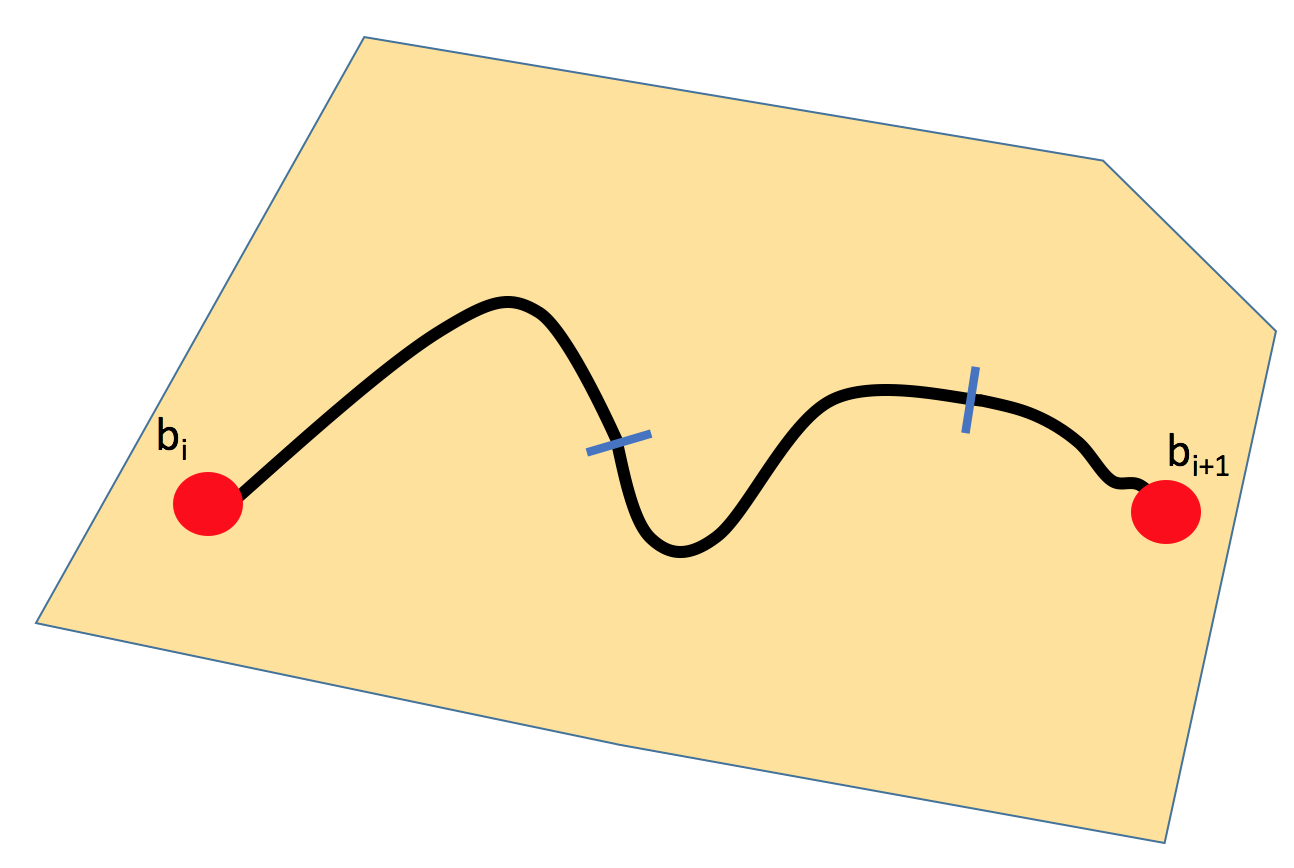
\includegraphics[width=.45\linewidth]{img/segmentiLinea}} \quad
	\subfloat[il colore del segmento tende sempre più al rosso all'aumentare del valore medio di \textit{exposure} dei punti al suo interno]
	{\label{mediaExposure}
		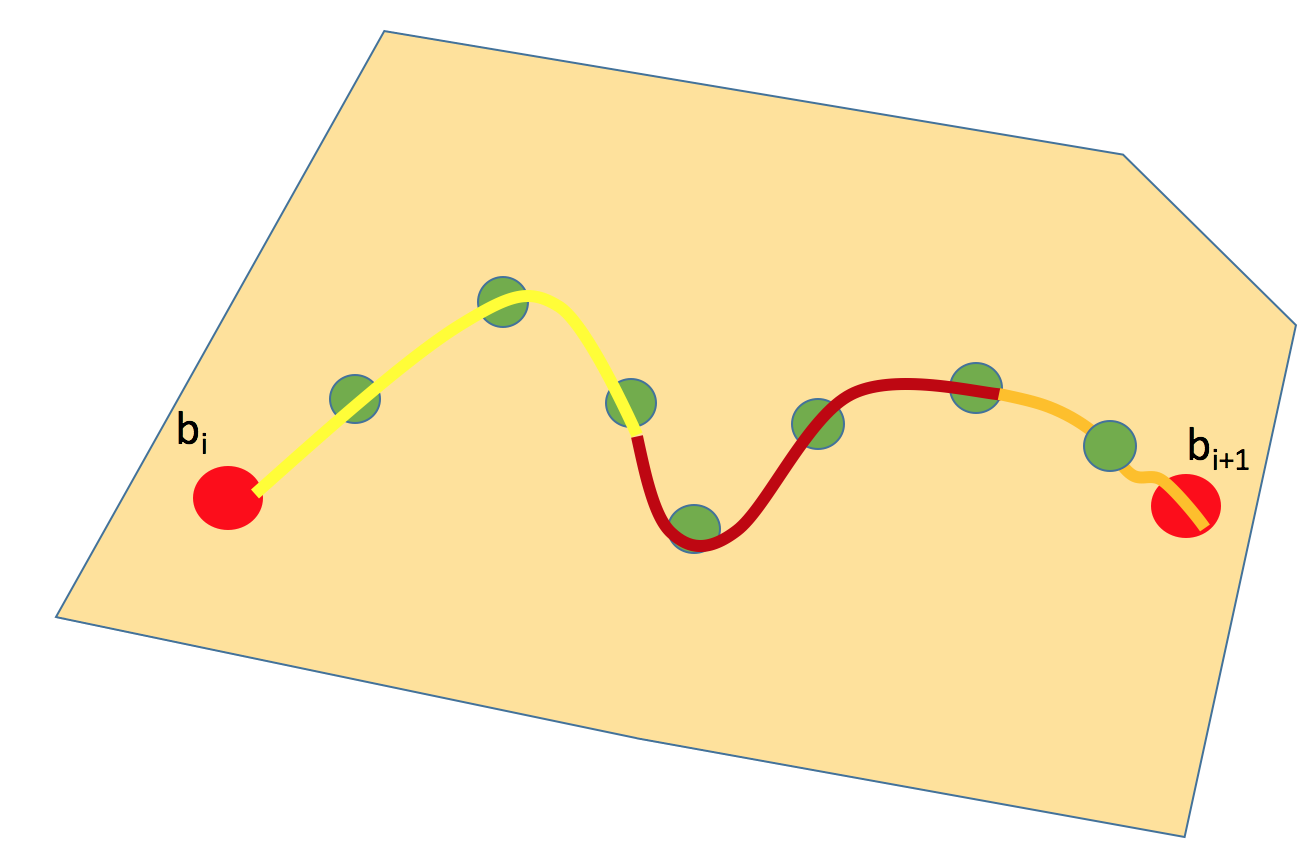
\includegraphics[width=.45\linewidth]{img/mediaExposure}} 
	\caption[dove]{Esempio di divisione di una linea ferroviaria (a) e assegnazione dell'exposure  ad ogni suo segmento (b) }
	\label{fig:aggregazioneLinea}
\end{figure}

Per ogni segmento si tiene traccia anche del valore massimo e della somma dell'\textit{exposure} dei punti al suo interno. Queste informazioni potrebbero in alcuni casi essere utili. Ad esempio se ci fosse un punto il cui valore di \textit{exposure} risulti essere molto alto rispetto gli altri punti, la media aritmetica non sarebbe sufficiente a rilevare tale situazione. 

\end{enumerate}




\subsection{L'algoritmo}
\chapter{Un caso di studio: L'Abruzzo}
\label{ch:casodistudio}

Il focus del presente studio è posto, come è stato già preannunciato in precedenza, unicamente sulla regione Abruzzo, la cui rete ferroviaria, nonostante non abbia una estensione considerevole, è immersa in un territorio eterogeneo ed esposto a diversi livelli di rischio di natura idrogeologica. La ridotta estensione dei dati in esame, ha consentito di focalizzarsi su una analisi puntuale e non dispersiva dei metodi proposti, al fine di valutarne accuratamente la validità ed i limiti. Il presente \textit{report} è stato prodotto a fronte di un lavoro di laboratorio volto alla costruzione dei seguenti dati:
\begin{itemize}
\item  Una classifica delle stazioni, in base al potenziale rischio idrogeologico a cui esse sono esposte;
\item  Una classifica dei tratti di ferrovia maggiormente esposti a rischio di smottamenti del terreno su cui sono posti i binari.
\end{itemize}{}
La produzione di tali classifiche ha l’obiettivo di consentire una fruibilità facile ed immediata dei dati per quegli enti preposti al monitoraggio e alla manutenzione delle tratte e stazioni ferroviarie.
\newline
Di seguito si mostrerà una breve istantanea della attuale situazione osservata nel territorio abruzzese, con particolare attenzione ai dati selezionati, tra quelli disponibili, e alla loro provenienza.
\section{Territorio}
L'Abruzzo (rappresentata in fig.\ref{fig:regioneAbruzzo}) è una regione a statuto ordinario dell'Italia peninsulare, compresa tra il mare Adriatico e l'Appennino centrale,con capoluogo L'Aquila. La regione è geograficamente ed economicamente parte dell'Italia centrale, mentre dal punto di vista storico e linguistico è inserita all'interno dell'Italia meridionale.
\newline
Occupa una superficie di 10.831 km² e ha una popolazione di 1.322.349 abitanti. È diviso in quattro province: L'Aquila, Chieti, Pescara e Teramo, e in 305 comuni. Confina a nord con le Marche, ad est con il mare Adriatico, ad ovest con il Lazio e a sud con il Molise. Si divide principalmente in una parte costiera nel versante orientale con le spiagge dell'Adriatico, e in una parte montuosa dal lato occidentale con il Gran Sasso d'Italia (2.914 m s.l.m.), la Majella (2.793 m s.l.m.) e il Sirente-Velino (2.487 m s.l.m.) che costituiscono i tre massicci montuosi più alti dell'intera catena appenninica.
\newpage
\begin{figure}[bht]
	\centering
	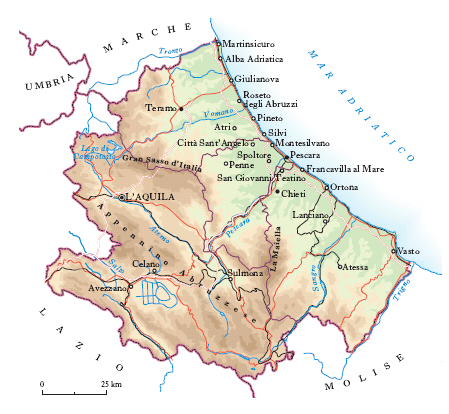
\includegraphics[width=0.4\textwidth]{img/regione}
	\caption{La regione Abruzzo}
    \label{fig:regioneAbruzzo}
\end{figure}

\section{Rete Ferroviaria}
Per quanto riguarda il trasporto ferroviario, vi è in Abruzzo una forte disparità tra quello moderno sulla costa (anche se con numero e qualità delle corse e del servizio imparagonabili rispetto all'asse ferroviario "tirrenico" e non è prevista alcuna linea di TAV) e quello delle zone interne, molto carente in termini di modernità e qualità del servizio e in attesa da decenni di interventi di potenziamento e ammodernamento (vedi in particolare la linea Pescara-Avezzano-Roma). Complessivamente comunque la rete ferroviaria abruzzese in attivo è abbastanza sviluppata e si estende per 524 km, mentre l'estensione totale complessiva della rete (attiva o dismessa) è pari a 648 km.

\subsection{Stazioni Ferroviarie}
I dati iniziali a nostra disposizione circa i nodi ferroviari ci forniscono le informazioni relative alle 114 stazioni distribuite sul territorio abruzzese mostrate in fig.\ref{fig:regioneStazione}.
\newpage
\begin{figure}[h]
	\centering
	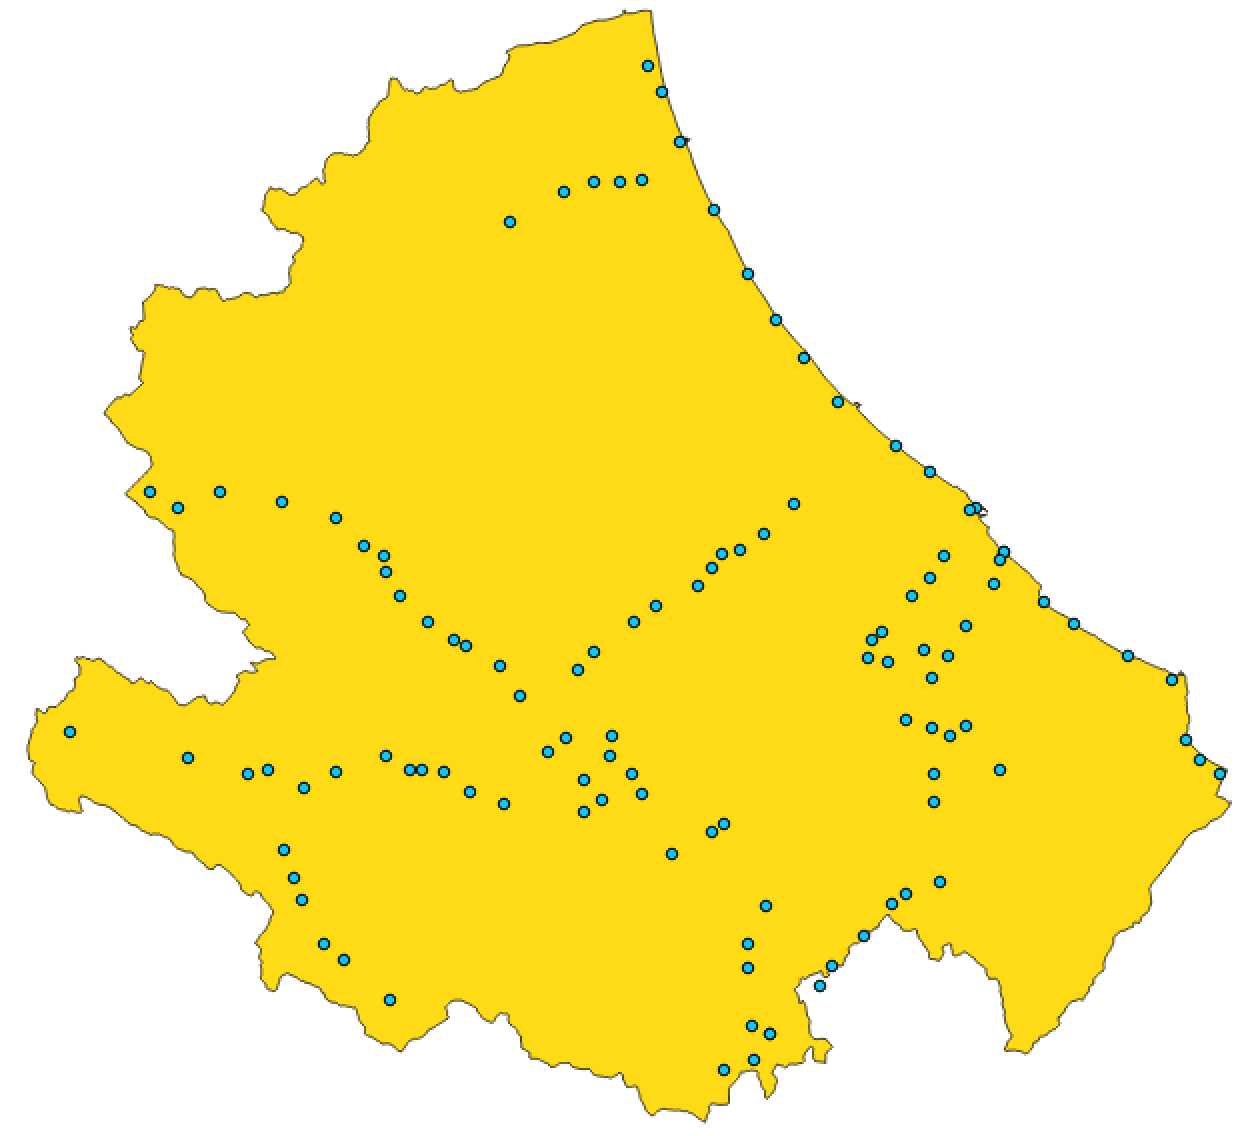
\includegraphics[width=0.4\textwidth]{img/regioneStazione}
	\caption{Stazioni ferroviarie presenti in Abruzzo}
    \label{fig:regioneStazione}
\end{figure}

\subsection{Linee Ferroviarie}
Sul territorio abruzzese sono presenti nove tratte ferroviarie:
\begin{itemize}
\item Bologna - Bari
\item Ortona - Crocetta
\item Marina di San Vito - Castel di Sangro
\item Roma - Pescara
\item Avezzano - Roccasecca
\item Archi stazione - Atessa
\item Sulmona - Carpinone
\item Rieti - L'Aquila - Sulmona
\item Teramo - Giulianova
\end{itemize}

\begin{figure}[h]
	\centering
	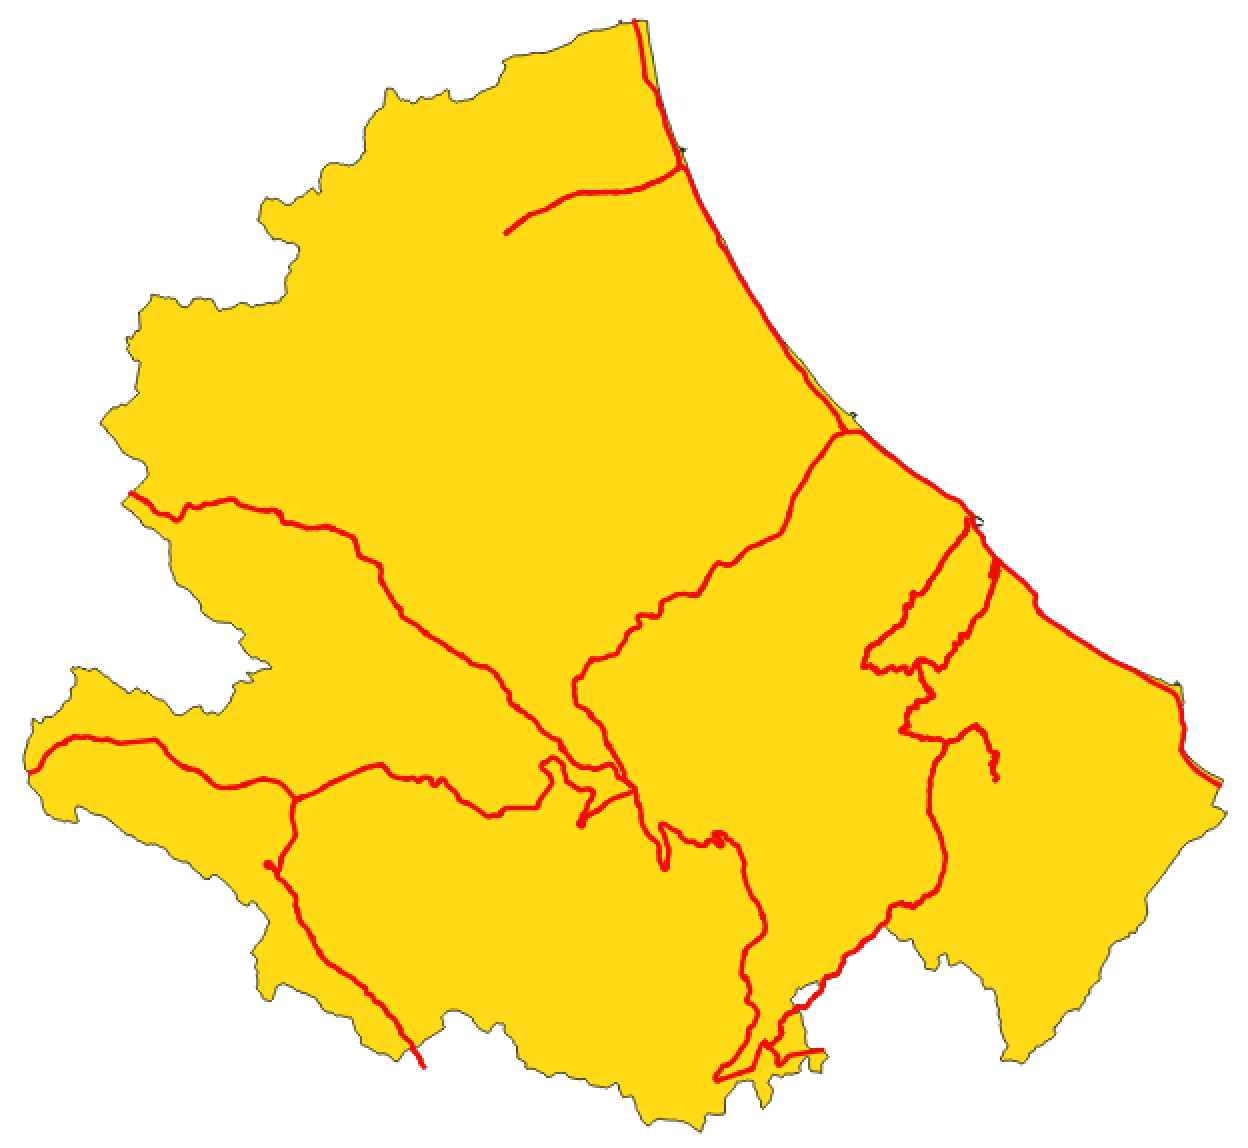
\includegraphics[width=0.4\textwidth]{img/regioneFerrovia}
	\caption{Linee ferroviarie presenti in Abruzzo}
    \label{fig:regioneFerrovia}
\end{figure}

Di queste tratte solo alcune sono completamente interne alla regione, altre invece la attraversano (avendo origine e/o fine al di fuori dei confini); riguardo queste ultime si è scelto di considerare unicamente le porzioni che cadono nella regione Abruzzo mostrate in fig.\ref{fig:regioneFerrovia}.
\newpage

\section{Zone}
\label{zone}
L'intero territorio abruzzese è stato completamente suddiviso in 22.000 zone più piccole la cui area media è pari a $0,5$ km$^2$. Il dataset relativo a queste zone ,che ci è stato fornito, è stato costruito mediante un algoritmo che segue un approccio basato sul \textit{diagramma di Voronoi}, tale da costruire una partizione completa del territorio determinata dalle distanze rispetto ad un determinato insieme discreto di elementi dello spazio (nel nostro caso un insieme finito di punti). Il risultato di tale partizionamento dello spazio è visibile nella Fig.\ref{fig:dataset}.
\begin{figure}[h]
	\centering
	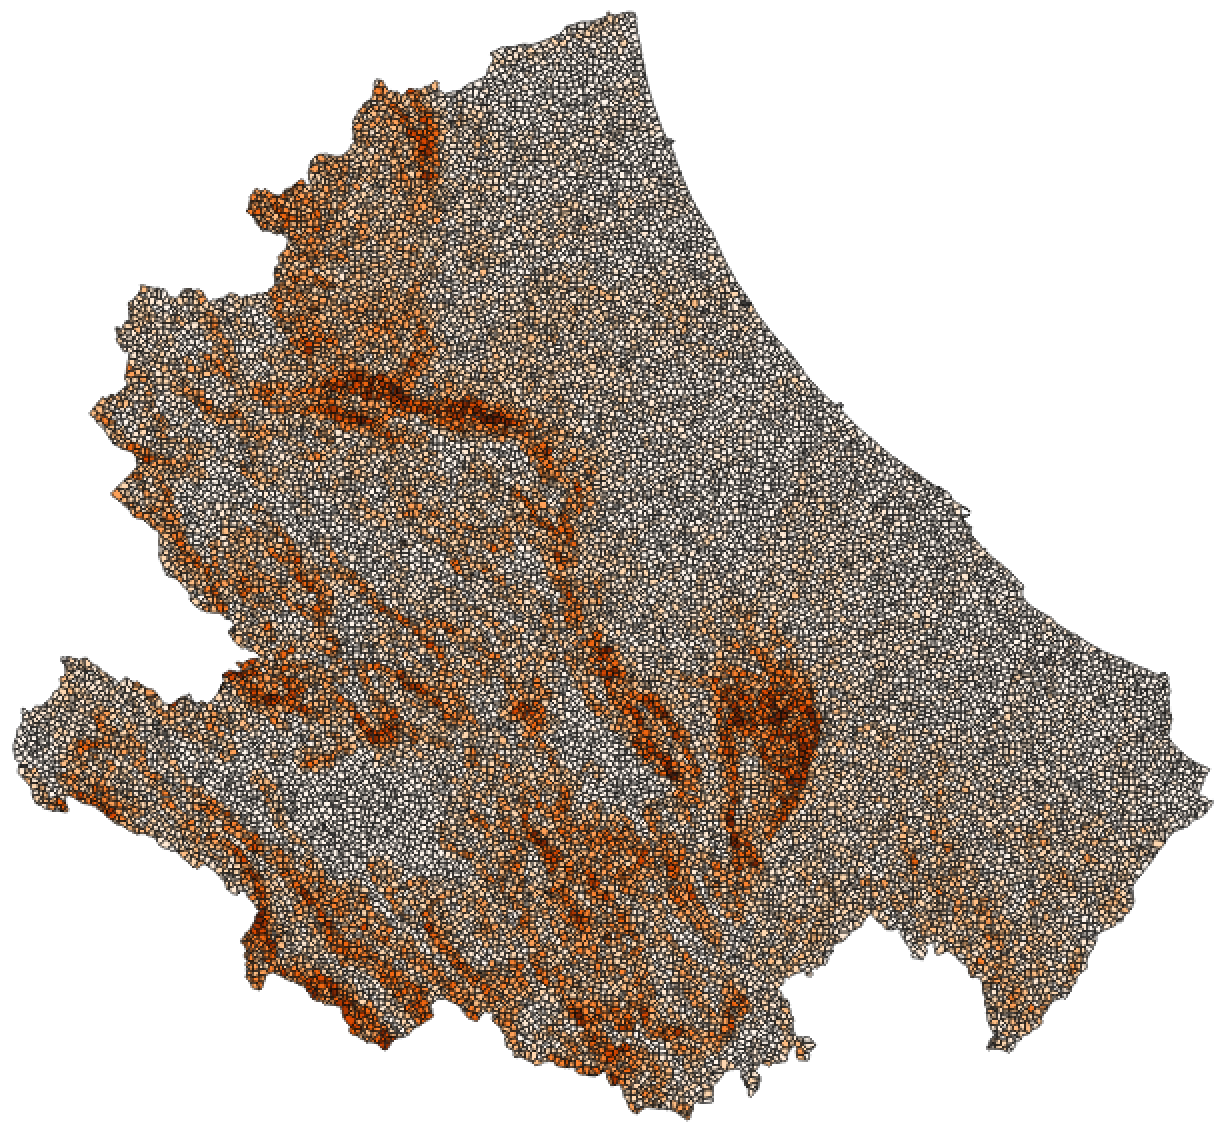
\includegraphics[width=0.5\textwidth]{img/dataset}
	\caption{Partizionamento completo della regione Abruzzo}
    \label{fig:dataset}
\end{figure}

Ad ogni $z_k$ è associato un valore numerico compreso tra $0$ e $1$, il quale quantifica la pericolosità determinata dal rischio idrogeologico della zona alla quale si riferisce.


%---------------
\section{Base di dati spaziale}
Si descrive in seguito la progettazione e conseguente realizzazione della base di dati geografica realizzata per l'effettiva implementazione degli algoritmi precedentemente descritti.\\
I dati da memorizzare sono: 
\begin{itemize}
\item alle stazioni e linee ferroviarie abruzzesi con informazioni relative al nome e alla geometria;
\item alla geometria dei confini dell'area geografica;
\item alla geometria delle zone che vanno a partizionare in modo completo l'area con relative informazioni di rischio idrogeologico;
\item alla geometria delle linee di livello presenti nel territorio di riferimento con la quota associata;
\item ai risultati ottenuti dalle elaborazioni.
\end{itemize}

 

\subsection{Progettazione concettuale}
Per ogni entità verranno mostrate:

\begin{itemize}
\item gli attributi
\item l'attributo identificante
\item i vincoli di partecipazione nelle relazioni, con la notazione (min, max)
\end{itemize}

In Figura \ref{fig:er} si riporta il modello E-R della base di dati spaziale, mentre in Tabella \ref{tab:erTabellaEntita} sono elencate le entità con i relativi attributi, descrizione e attributi identificanti, ed infine in Tabella \ref{tab:erTabellaAssociazioni} l’elenco delle associazioni.
\pagebreak

\begin{figure}[h]
	\centering
	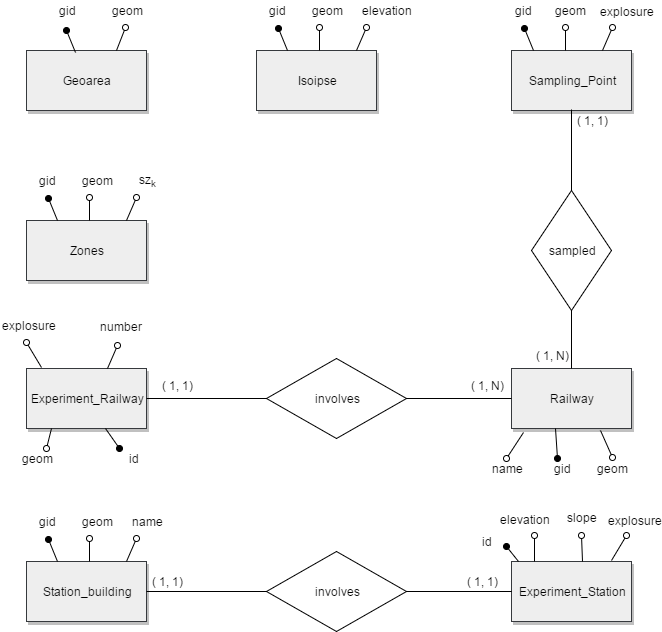
\includegraphics[width=1\textwidth]{img/er}
	\caption{Diagramma E-R della base di dati}
    \label{fig:er}
\end{figure}

Note:\\
l'attributo \textit{number} dell'entità \textit{Experiment\_railway}  rappresenta il numero del segmento relativo alla linea ferroviaria di appartenenza. Nel caso di divisione delle linee in tratte da 1 km,  corrisponde anche al km lungo la tratta.
\pagebreak

\begin{table}[h]
\centering
\begin{tabular}{|c|c|c|c|}
\hline
\textbf{Entità} & \textbf{Descrizione} & $\mathbf{Attributi}$ & \textbf{ID} \\
\hline

\multirow{3}{*}\textit{Geoarea} & Entità relativa al territorio di & \textit{gid} & \textit{gid}\\
& interesse. Nel nostro caso è la & \textit{geom} & \\&regione Abruzzo.&&\\ 
\hline

\multirow{3}{*}\textit{Zones} & Entità relativa al territorio di & \textit{gid} & \textit{gid}\\
& interesse. Nel nostro caso è un & \textit{sz$_k$} & \\
& partizionamento completo della &\textit{geom}& \\ 
& regione Abruzzo.&&\\ \hline

\multirow{3}{*}\textit{Station\_building} & Entità relativa alle stazioni & \textit{gid} & \textit{gid}\\
& presenti nel territorio di & \textit{name} & \\
& riferimento. &\textit{geom}& \\  \hline

\multirow{3}{*}\textit{Isoipse} & Entità relativa alle isoipse & \textit{gid} & \textit{gid}\\
& presenti nel territorio di & \textit{elevation} & \\
& riferimento. &\textit{geom}& \\  \hline

\multirow{3}{*}\textit{Railway} & Entità relativa alle linee ferroviarie & \textit{gid} & \textit{gid}\\
& presenti nel territorio di & \textit{name} & \\
& riferimento. &\textit{geom}& \\  \hline

\multirow{3}{*}\textit{Sampling\_point} & Entità relativa ai punti individuati & \textit{id} & \textit{id}\\
& come campionamento delle linee  & \textit{geom} & \\
&  ferroviarie presenti nel territorio &\textit{explosure}& \\
&  di riferimento. && \\  \hline

\multirow{4}{*}\textit{Experiment\_station} & Entità relativa agli esperimenti & \textit{id} & \textit{id}\\
& effettuati sulle stazioni & \textit{elevation} & \\
& presenti nel territorio& \textit{slope} & \\
& di riferimento. &\textit{explosure}& \\ \hline

\multirow{4}{*}\textit{Experiment\_railway} & Entità relativa agli esperimenti & \textit{id} & \textit{id}\\
& effettuati sulle linee ferroviarie  & \textit{geom} & \\
& presenti nel territorio &\textit{numero}& \\
& di riferimento. & \textit{explosure}&\\ \hline

\end{tabular}
\caption{Tabella delle entità}
\label{tab:erTabellaEntita}
\end{table}

\begin{table}[h]
\centering
\begin{tabular}{|c|c|c|c|}
\hline
\textbf{Associazione} & \textbf{Descrizione} & $\mathbf{Entità\ coinvolte}$ & \textbf{Attributi} \\
\hline

\multirow{3}{*}\textit{involves} & Relazione che evidenzia il & \textit{station\_building} & \textit{nessuna}\\
& coinvolgimento di una sola & \textit{experiment\_station} & \\
& stazione in ogni esperimento. && \\ \hline

\multirow{3}{*}\textit{implicated} & Relazione che evidenzia il  & \textit{railway} & \textit{nessuna}\\
& coinvolgimento di almeno una & \textit{experiment\_railway} & \\
& linea ferroviaria in uno o &&\\ 
& più esperimenti.&&\\
\hline

\multirow{3}{*}\textit{sampled} & Relazione che lega ogni linea & \textit{railway} & \textit{nessuna}\\
& ferroviaria con uno o più punti & \textit{sampling\_point} & \\
& di campionamento. &&\\ 
\hline

\end{tabular}
\caption{Tabella delle associazioni}
\label{tab:erTabellaAssociazioni}
\end{table}
\clearpage

\subsection{Progettazione logica}
Il diagramma E-R in figura \ref{fig:er} viene tradotto nello schema logico rappresentato graficamente in figura \ref{fig:schemaLogico}

\begin{figure}[h]
	\centering
	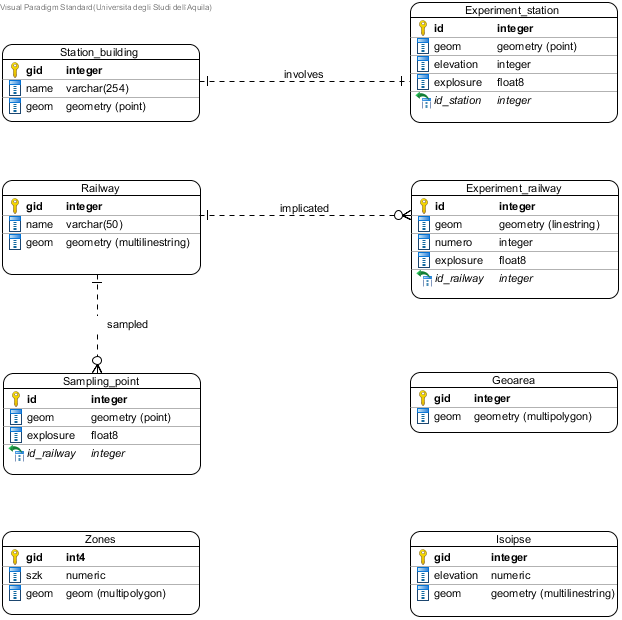
\includegraphics[width=1\textwidth]{img/schemaLogico}
	\caption{Schema logico}
    \label{fig:schemaLogico}
\end{figure}

\chapter{Risultati e loro discussione} 
\label{ch:risultatiediscussione} 

Nella sezione \ref{ch:risultatiediscussione} verranno illustrati i risultati più significativi ottenuti dall'applicazione dei metodi esposti (vedi Sez.\ref{ch:materialandmethods}) per il calcolo del ranking, rispettivamente delle stazioni e delle tratte ferroviarie.
Per i risultati completi si rimanda alla lettura dell'appendice \ref{risultati}.
\section{Ranking e  Valutazione delle stazioni ferroviarie}

Applicando il metodo discusso nella Sez. \ref{metodoNuovo} abbiamo ottenuto i risultati che andremo qui di seguito ad illustrare.
Tali risultati sono stati utilizzati per realizzare una classifica delle stazioni in base al loro grado di esposizione al pericolo idrogeologico.

%inserire parte introduttiva che richiama i dati in analisi a quale tabella/colonna appartengono della bd..

Il valore di \textit{exposure} ottenuto per le stazioni in analisi  varia da un valore minimo di $0$ ad un massimo di $50$. A fronte di tali risultati si è deciso di definire tre diverse fasce di esposizione al pericolo in base alle quali aggregare le stazioni all'interno della classifica:
\begin{itemize}
\item \textit{High}
\item \textit{Moderate}
\item \textit{Low}
\end{itemize}
La Tabella n°\ref{range} mostra la suddetta suddivisione in fasce di rischio, gli intervalli in cui le stazioni sono state divise secondo il valore di \textit{exposure}, il numero e la percentuale sul totale delle stazioni appartenenti ad una determinata fascia. Inoltre ad ogni fascia è stato associato un colore identificativo.
\begin{table}[h]
\centering
\begin{tabular}{|c|c|c|c|}
\hline
\rowcolor{lightgray}
\textbf{Fascia} & \textbf{Intervallo valori Exp$\mathbf{\_}$$\mathbf{b_i}$} & $\mathbf{\#b_i}$ & \textbf{\%} \\
\hline
\rowcolor{flamingopink}
High & 20 < Exp$\_$$b_i$ < 50 & 6 & 5,26\%\\
\hline
\rowcolor{icterine}
Moderate & 1 < Exp$\_$$b_i$ < 20 & 62 & 54,39\%\\
\hline
\rowcolor{inchworm}
Low & $0$ < Exp$\_$$b_i$ < 1 & 46 & 40,35\%\\
\hline
\end{tabular}
\caption{Aggregazione delle stazioni $b_i$ in base al valore di \textit{exposure} }
\label{range}
\end{table}

Come si evince dalla tabella \ref{range} tale suddivisione in fasce non è lineare ma bensì frutto di un'analisi critica (vedi Sez.  \ref{analisicritica}) del metodo discusso (vedi Sez. \ref{metodoNuovo}) e dei risultati ottenuti. Inoltre è possibile notare come la maggioranza delle stazioni presenta un livello di esposizione al rischio \textit{Moderate} mentre solo il 5,26\% presenta valori di \textit{exposure} tali da far emergere il bisogno di controlli più frequenti (fascia \textit{High}).

Nella tabella \ref{classifica} si riportano i primi dieci record, appartenenti alla classifica delle stazioni ordinati in modo decrescente rispetto il valore di \textit{exposure}. In riferimento alla singola stazione, per ogni record vengono quindi mostrati la posizione all'interno della classifica, l'identificativo, il nome e il suo valore di \textit{exposure}.

\begin{table}[h]
\centering
\begin{tabular}{|c|c|c|c|}
\hline
\rowcolor{lightgray}
\textbf{n.} & \textbf{id Stazione} & \textbf{Nome Stazione Ferroviaria} & \textbf{Valore di \textit{exposure}} \\
\hline
\rowcolor{flamingopink}
1 & 114 & Acciano & 49,85 \\
\hline
\rowcolor{flamingopink}
2 & 54 & Fontecchio & 42,68 \\
\hline
\rowcolor{flamingopink}
3 & 44 & Sant'Ilario & 31,73 \\
\hline
\rowcolor{flamingopink}
4 & 38 & Pettorano Sul Gizio & 31,14 \\
\hline
\rowcolor{flamingopink}
5 & 94 & Isca d'Archi & 22,71 \\
\hline
\rowcolor{flamingopink}
6 & 66 & Prezza & 20,54 \\
\hline
\rowcolor{icterine}
7 & 33 & Bussi & 19,98 \\
\hline
\rowcolor{icterine}
8 & 81 & Capistrello & 18,57 \\
\hline
\rowcolor{icterine}
9 & 91 & Civitaluparella & 16,32 \\
\hline
\rowcolor{icterine}
10 & 63 & Sella di Corno & 14,24 \\
\hline
\end{tabular}
\caption{Classifica delle prime dieci stazioni ordinata in base al valore di \textit{exposure}}
\label{classifica}
\end{table}
%inserire appendice dove sta la classificazione ufficiale
%discutere se inserire l'ordinamento della classifica ufficiale
\subsection{Analisi critica del Nuovo Metodo Proposto}
\label{analisicritica}
Osservando i risultati ottenuti dall'applicazione del metodo di cui abbiamo discusso nella Sez. \ref{metodoNuovo} abbiamo potuto osservare come i valori di \textit{exposure} delle stazioni ferroviarie non presentano una distribuzione\newline "\textit{omogenea/lineare}" lungo l'asse dei numeri reali bensì risultano "aggregati" in gruppi di valori i quali ci hanno guidato nella definizione dei range di valori per ogni fascia che abbiamo presentato nella Tab. \ref{range}.
Il NMC restituisce valori in , quindi utilizzare un'equazione lineare per aggregare le stazioni in 3 fasce in base al loro valore di \textit{exposure} risulterebbe errato.
Al fine di poter valutare le performance del metodo proposto nella Sez. \ref{metodoNuovo} abbiamo confrontato la classificazione in fasce delle stazioni ottenuta in base ai valori di \textit{exposure} con la classificazione in fasce delle stazioni ferroviarie presenti sul territorio realizzata dai membri dei gruppi partecipanti al Laboratorio di Basi di Dati II nell'A.A. 2016/2017 tramite un'indagine visiva del territorio ove tali edifici sono situati. L'ipotesi di lavoro implicita è che tale classificazione "umana", indicata d'ora in avanti come classificazione ufficiale, sia corretta per definizione. Pertanto i risultati ottenuti dal metodo discusso nella Sez. \ref{metodoNuovo} saranno tanto più soddisfacenti quanto più questi si avvicineranno ai dati ufficiali.

La tabella che riporta la classificazione in fasce ufficiale delle stazioni ferroviarie nella sua completezza è presente in appendice \ref{risultatiUfficiali}, mentre qui di seguito, in tabella \ref{fasciaHighUfficiale}, sono stati riportati i record delle stazioni che sono stati classificati ufficialmente in fascia \textit{High}.
\begin{table}[h]
\centering
\begin{tabular}{|c|c|}
\hline
\rowcolor{lightgray}
\textbf{id Stazione} & \textbf{Nome Stazione Ferroviaria} \\
\hline
\rowcolor{flamingopink}
44 & Sant'Ilario \\
\hline
\rowcolor{flamingopink}
65 & Aversa \\\hline
\rowcolor{flamingopink}
54 & Fontecchio \\\hline
\rowcolor{flamingopink}
38 & Pettorano sul Gizio \\\hline
\rowcolor{flamingopink}
114 & Acciano \\\hline
\rowcolor{flamingopink}
62 & Vigliano d'Abruzzo \\
\hline
\end{tabular}
\caption{Elenco delle stazioni ferroviarie ufficialmente in fascia \textit{High}}
\label{fasciaHighUfficiale}
\end{table}

Lo studio delle performance del metodo è stato realizzato mediante la \textit{tabella di contingenza} (detta anche \textit{matrice di errore} o \textit{di confusione}). Ogni colonna di tale tabella rappresenta le istanze in una fascia "prevista" (\textit{Predicted Classes}) mentre le righe rappresentano le istanze in una fascia reale (\textit{Actual Classes}). La corrispondente \textit{tabella di contingenza} (tabella \ref{tabellaContingenza}) riassume i risultati ottenuti con il metodo. 

\begin{table}[h]
\centering
\begin{tabular}{|cc|c|c|c|c|}
\hline
\multicolumn{2}{|c|}{\multirow{2}*{}} & \multicolumn{3}{c|}{Predicted Classes} & \multirow{2}*{Totale} \\
\cline{3-5}
 & & High & Moderate & Low &  \\
\hline
\multicolumn{1}{|c|}{\multirow{3}*{Actual Classes}} & High & $4$ & $2$ & $0$ & 6 \\
\cline{2-6}
\multicolumn{1}{|c|}{}& Moderate & $2$ & $53$ & $6$ & $61$ \\
\cline{2-6}
\multicolumn{1}{|c|}{}& Low & $0$ & $7$ & $40$ & $47$ \\
\hline
\multicolumn{2}{|c|}{Totale}& $6$ & $62$ & $46$ & $114$ \\
\hline
\end{tabular}
\caption{\textit{Tabella di Contingenza} del metodo NMC discusso nella Sez. \ref{metodoNuovo}}
\label{tabellaContingenza}
\end{table}

Osservando i dati contenuti nella tabella \ref{tabellaContingenza} è possibile ricavare le seguenti deduzioni:
\begin{itemize}
\item Delle 6 stazioni classificate ufficialmente in fascia \textit{High} il metodo ha previsto che 2 di queste sono in fascia \textit{Moderate};
\item Delle 61 stazioni classificate ufficialmente in fascia \textit{Moderate} il metodo ha previsto che 2 di queste sono in fascia \textit{High} mentre 6 sono in fascia \textit{Low};
\item Delle 47 stazioni classificate ufficialmente in fascia \textit{Low} il metodo ha previsto che 7 sono in fascia \textit{Moderate};
\item Le stazioni correttamente classificate dal nostro metodo sono localizzate lungo la diagonale della tabella.
\end{itemize}

Dall'esame della \textit{letteratura} del settore del \textit{Machine Learning} emerge che la maniera più semplice di effettuare misurazioni circa le performance della predizione restituita dal metodo adottato consiste nel ricondurre il problema della classificazione dei risultati ottenuti al caso di \textit{tabella di contingenza binaria}, ossia al caso nel quale sia coinvolta una sola classe alla volta. Il problema può essere quindi formulato come segue:
\newline
\newline
\textit{Dati n valori (v1, v2, …, vn) e una classe (C), costruire la tabella di contingenza binaria che riassume
come detti valori sono classificati sia nel mondo reale che secondo quanto stimato dall’algoritmo del
quale si vuole misurare la efficacia. Evidentemente il valore v1 potrà cadere in C oppure no, idem per
v2, …., vn.}
\newline
\newline
Dalla tabella \ref{tabellaContingenza} è possibile ricavare le seguenti \textit{tabelle di contingenza} riferite relativamente alla fascia \textit{High} (Tabella \ref{tabellaHigh}), alla fascia \textit{Moderate} (Tabella \ref{tabellaModerate}) e alla fascia \textit{Low} (Tabella \ref{tabellaLow}).

\begin{table}[h]
\centering
\begin{tabular}{|cc|c|c|c|}
\hline
\multicolumn{2}{|c|}{\multirow{2}*{}} & \multicolumn{2}{c|}{Predicted Classes} & \multirow{2}*{Totale} \\
\cline{3-4}
 & & High & Not High &  \\
\hline
\multicolumn{1}{|c|}{\multirow{2}*{Actual Classes}} & High & $4$  & $2$ & 6 \\
\cline{2-5}

\multicolumn{1}{|c|}{}& Not High  & $2$ & $106$ & $108$ \\
\hline
\multicolumn{2}{|c|}{Totale}& $6$ & $108$ & $114$ \\
\hline
\end{tabular}
\caption{\textit{Tabella di contingenza binaria} riferita alla fascia \textit{High} }
\label{tabellaHigh}
\end{table}

\textbf{Segue un commento alla tabella \ref{tabellaHigh}}

Prima Riga:
\begin{itemize}
\item Il numero 4 denota le stazioni che il metodo ha classificato correttamente in fascia \textit{High} (da questo
momento chiameremo questi casi \textit{Veri Positivi});
\item Il numero 2 denota le stazioni che il metodo \textbf{non} ha classificato \textbf{correttamente} in fascia \textit{High} ma in un'altra fascia  (da questo momento chiameremo questi casi \textit{Falsi
Negativi}).
\end{itemize}

Seconda Riga:
\begin{itemize}
\item Il numero 2 denota i casi nei quali l’algoritmo ha classificato \textbf{erroneamente} delle stazioni in classe \textit{High} (da
questo momento chiameremo questi casi \textit{Falsi Positivi});
\item Il numero 106 denota le stazioni che l’algoritmo ha classificato correttamente come \textbf{non} di classe \textit{High} (da questo momento chiameremo questi casi \textit{Veri Negativi}).
\end{itemize}
\newpage
\begin{table}[h]
\centering
\begin{tabular}{|cc|c|c|c|}
\hline
\multicolumn{2}{|c|}{\multirow{2}*{}} & \multicolumn{2}{c|}{Predicted Classes} & \multirow{2}*{Totale} \\
\cline{3-4}
 & & Moderate & Not Moderate &  \\
\hline
\multicolumn{1}{|c|}{\multirow{2}*{Actual Classes}} & Moderate & $53$  & $8$ & 61 \\
\cline{2-5}

\multicolumn{1}{|c|}{}& Not Moderate  & $9$ & $44$ & $53$ \\
\hline
\multicolumn{2}{|c|}{Totale}& $62$ & $52$ & $114$ \\
\hline
\end{tabular}
\caption{\textit{Tabella di contingenza binaria} riferita alla fascia \textit{Moderate} }
\label{tabellaModerate}
\end{table}

\textbf{Segue un commento alla tabella \ref{tabellaModerate}}

Prima Riga:
\begin{itemize}
\item Il numero 53 denota le stazioni che il metodo ha classificato correttamente in fascia \textit{Moderate};
\item Il numero 8 denota le stazioni che il metodo \textbf{non} ha classificato \textbf{correttamente} in fascia \textit{Moderate} ma in un'altra fascia.
\end{itemize}

Seconda Riga:
\begin{itemize}
\item Il numero 9 denota i casi nei quali l’algoritmo ha classificato \textbf{erroneamente} delle stazioni in classe \textit{Moderate};
\item Il numero 44 denota le stazioni che l’algoritmo ha classificato correttamente come \textbf{non} di classe \textit{Moderate}.
\end{itemize}

\begin{table}[h]
\centering
\begin{tabular}{|cc|c|c|c|}
\hline
\multicolumn{2}{|c|}{\multirow{2}*{}} & \multicolumn{2}{c|}{Predicted Classes} & \multirow{2}*{Totale} \\
\cline{3-4}
 & & Low & Not Low &  \\
\hline
\multicolumn{1}{|c|}{\multirow{2}*{Actual Classes}} & Low & $40$  & $7$ & 47 \\
\cline{2-5}

\multicolumn{1}{|c|}{}& Not Low  & $6$ & $61$ & $67$ \\
\hline
\multicolumn{2}{|c|}{Totale}& $46$ & $68$ & $114$ \\
\hline
\end{tabular}
\caption{\textit{Tabella di contingenza binaria} riferita alla fascia \textit{Low} }
\label{tabellaLow}
\end{table}

\textbf{Segue un commento alla tabella \ref{tabellaLow}}

Prima Riga:
\begin{itemize}
\item Il numero 40 denota le stazioni che il metodo ha classificato correttamente in fascia \textit{Low};
\item Il numero 7 denota le stazioni che il metodo \textbf{non} ha classificato \textbf{correttamente} in fascia \textit{Low} ma in un'altra fascia;
\end{itemize}

Seconda Riga:
\begin{itemize}
\item Il numero 6 denota i casi nei quali l’algoritmo ha classificato \textbf{erroneamente} delle stazioni in classe \textit{Low};
\item Il numero 61 denota le stazioni che l’algoritmo ha classificato correttamente come \textbf{non} di classe \textit{Low}.
\end{itemize}

Prima di elencare le metriche che abbiamo adottato per giudicare le performance del metodo è utile introdurre la tabella \ref{tabellaParametri}, nella quale andremo ad evidenziare i sei parametri che descrivono la \textit{tabella di contingenza binaria}, ovvero: P, N, VP, FP, FN, VN, a ciascuno dei quali corrisponde un valore intero.

In letteratura sono state proposte molte metriche per giudicare le performance di un algoritmo che restituisca la realtà osservata, le più diffuse verranno elencate di seguito. Si segnala inoltre che il valore di ciascuna di essere esprime una probabilità, quindi oscilla tra $0$ e $1$.

\begin{table}[h]
\centering
\begin{tabular}{|cc|c|c|c|}
\hline
\multicolumn{2}{|c|}{\multirow{2}*{}} & \multicolumn{2}{c|}{Predicted Classes} & \multirow{2}*{Totale} \\
\cline{3-4}
 & & Predizione Affermativa & Predizione Falsa &  \\
\hline
\multicolumn{2}{|c|}{\multirow{4}*{Actual Classes}} & \multirow{2}*{Veri Positivi }  & \multirow{2}*{Falsi Negativi}  & \multirow{2}*{Valori $\in$ alla classe}\\
&&(\textbf{VP})&(\textbf{FN})&\textbf{P=VP + FN} \\
\cline{3-5}

\multicolumn{2}{|c|}{}& \multirow{2}*{Falsi Positivi}  & \multirow{2}*{Veri Negativi}  & \multirow{2}*{Totali altri valori} \\
&&(\textbf{FP})&(\textbf{VN})& \textbf{N=FP+VN}\\
\hline

\multicolumn{2}{|c|}{\multirow{2}*{Totale}}& \multirow{2}*{VP + FP} & \multirow{2}*{FN + VN} & \multirow{2}*{P + N =}\\
&&&&VP + FP + FN + VN \\
\hline
\end{tabular}
\caption{\textit{Tabella di contingenza binaria} "neutra" }
\label{tabellaParametri}
\end{table}

La \textbf{Percentuale dei Veri Positivi} (True Positive Rate) è definita come la percentuale dei casi positivi riconosciuti (dal metodo di classificazione adottato) correttamente come tali. E' auspicabile che tale valore sia prossimo a 1. In formule:
\begin{equation}
\centering
PVP = {VP \over P} = {VP \over {(VP + FN)}}
\label{pvp}
\end{equation}

Dalle \textit{tabelle di contingenza binaria} relative relativamente alla fascia \textit{High}, alla fascia \textit{Moderate} e alla fascia \textit{Low} otteniamo i seguenti valori di PVP:
\begin{itemize}
\item PVP fascia \textit{High} = $0,67$
\item PVP fascia \textit{Moderate} = $0,87$
\item PVP fascia \textit{Low} = $0,85$
\end{itemize}

La \textbf{Percentuale dei Falsi Negativi} (False Negative Rate) o Percentuale dei Mancati Allarmi è definita in formule come segue:
\begin{equation}
\centering
PFN = {FN \over P} = {FN \over {(VP + FN)}} = {1 – PVP}
\label{pfn}
\end{equation}
Dalla formula si evince che esso è il complementare a PVP, ovvero che è auspicabile che il suo valore tenda a $0$.

Dalle \textit{tabelle di contingenza binaria} riferite relativamente alla fascia \textit{High}, alla fascia \textit{Moderate} e alla fascia \textit{Low} otteniamo i seguenti valori di PFN:
\begin{itemize}
\item PFN fascia \textit{High} = $0,33$
\item PFN fascia \textit{Moderate} = $0,13$
\item PFN fascia \textit{Low} = $0,15$
\end{itemize}

La \textbf{Percentuale dei Veri Negativi} (True Negative Rate) indica la percentuale dei casi che non destano allarme. In formule:
\begin{equation}
PVN = {VN \over N} = {VN \over {(FP + VN)}}
\end{equation}

Dalle \textit{tabelle di contingenza binaria} riferite relativamente alla fascia \textit{High}, alla fascia \textit{Moderate} e alla fascia \textit{Low} otteniamo i seguenti valori di PVN:
\begin{itemize}
\item PVN fascia \textit{High} = $0,98$
\item PVN fascia \textit{Moderate} = $0,83$
\item PVN fascia \textit{Low} = $0,91$
\end{itemize}

La \textbf{Percentuale dei Falsi Positivi} (False Positive Rate) indica la percentuale di falsi allarmi. In formule:
\begin{equation}
PFP = FP / N = FP / (FP + VN) = 1 - PVN
\end{equation}

Dalle \textit{tabelle di contingenza binaria} riferite relativamente alla fascia \textit{High}, alla fascia \textit{Moderate} e alla fascia \textit{Low} otteniamo i seguenti valori di PFP:
\begin{itemize}
\item PFP fascia \textit{High} = $0,02$
\item PFP fascia \textit{Moderate} = $0,17$
\item PFP fascia \textit{Low} = $0,09$
\end{itemize}

La \textbf{Precisione} è definita dalla seguente formula:
\begin{equation}
P = {VP \over {(VP + FP)}}
\end{equation}

Dalle \textit{tabelle di contingenza binaria} riferite relativamente alla fascia \textit{High}, alla fascia \textit{Moderate} e alla fascia \textit{Low} otteniamo i seguenti valori di Precisione:
\begin{itemize}
\item Precisione fascia \textit{High} = $0,67$
\item Precisione fascia \textit{Moderate} = $0,85$
\item Precisione fascia \textit{Low} = $0,87$
\end{itemize}

L' \textbf{Accuratezza} è definita dalla seguente formula:
\begin{equation}
ACC = {{(VP + VN)} \over {(P + N)} }= {{(VP + VN)} \over {((VP + FN) + (VN + FP))}}
\end{equation}

Dalle \textit{tabelle di contingenza binaria} riferite relativamente alla fascia \textit{High}, alla fascia \textit{Moderate} e alla fascia \textit{Low} otteniamo i seguenti valori di Accuratezza:
\begin{itemize}
\item Accuratezza fascia \textit{High} = $0,89$
\item Accuratezza fascia \textit{Moderate} = $0,85$
\item Accuratezza fascia \textit{Low} = $0,89$
\end{itemize}
%----------------------------------
\subsection{Discussione dei risultati ottenuti}
\label{discussioneRisultati}
Alla luce dei risultati ottenuti dal confronto tra la classificazione in fasce ottenuta dall'elaborazione dell'output del metodo illustrato nella Sez. \ref{metodoNuovo} e la classificazione ufficiale e dai valori delle metriche utilizzate per valutare le performance del metodo proposto è stato possibile concludere che l'algoritmo presenta sì alcune limitazioni che andremo a discutere qui di seguito ma che ha buone performance e riesce generalmente (nell'87\% dei casi) a classificare correttamente le stazioni ferroviarie presenti sul territorio abruzzese.

Le limitazioni del metodo proposto derivano dal fatto che l'algoritmo, nel calcolare il \textit{vettoreDirezionale}, prende in considerazione la curva di livello più vicina alla stazione ferroviaria a cui si riferisce e non sempre coincide con la direzione lungo la quale si propaga la pendenza più rilevante presente nelle vicinanze della stazione. Per maggiore chiarezza, qui di seguito, portiamo in esame due casi critici nei quali questa limitazione è ben visibile:
\begin{itemize}
\item \textbf{Aversa}
\newline La stazione ferroviaria di Aversa viene classificata dal nostro metodo in fascia \textit{Moderate} mentre \textit{ufficialmente} viene classificata in fascia \textit{High}. In figura \ref{fig:aversa} è visibile come il  \textit{vettoreDirezionale} viene costruito considerando la curva di livello più vicina (a 68m) al punto che indica la stazione di Aversa mentre il pendio con una pendenza maggiore si riferisce alla curva di livello che dista 93m dal punto. Ragion per cui, il valore di \textit{exposure} ottenuto applicando il metodo proposto nella Sez. \ref{metodoNuovo} per questa stazione ferroviaria è tale da classificare erroneamente tale edificio in fascia \textit{Moderate}. 
\newpage
\begin{figure}[bth]
\myfloatalign
\subfloat[]
{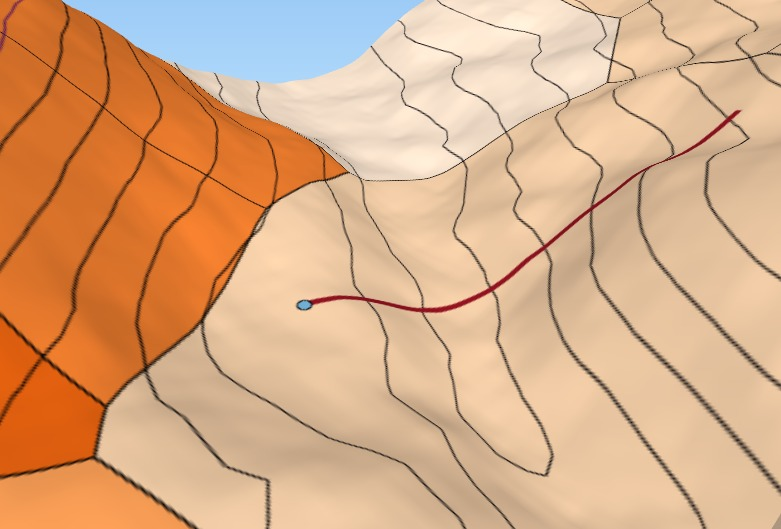
\includegraphics[width=0.4\linewidth]{img/Aversa}} \quad
\subfloat[]
{\label{fig:aversa-b}
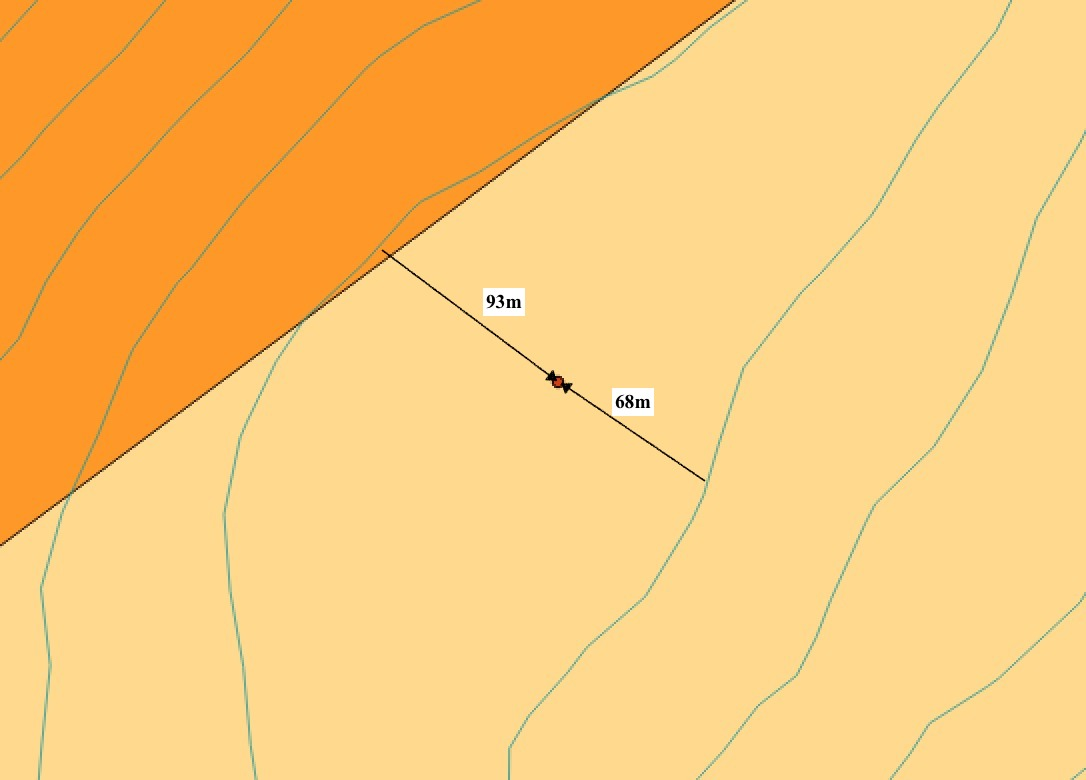
\includegraphics[width=0.38\linewidth]{img/Aversa2}} 
\caption[]{Stazione Ferroviaria di Aversa}\label{fig:aversa}
\end{figure}
\item \textbf{Vigliano d'Abruzzo}
\newline La stazione ferroviaria di Vigliano d'Abruzzo viene classificata dal nostro metodo in fascia \textit{Moderate} mentre \textit{ufficialmente} viene classificata in fascia \textit{High}. In figura \ref{fig:vigliano} è visibile come il  \textit{vettoreDirezionale} viene costruito considerando la curva di livello più vicina (a 38m) al punto che indica la stazione di Aversa mentre il pendio con una pendenza maggiore si riferisce alla curva di livello che dista 56m dal punto. Ragion per cui, il valore di \textit{exposure} ottenuto applicando il metodo proposto nella Sez. \ref{metodoNuovo} per questa stazione ferroviaria è tale da classificare erroneamente tale edificio in fascia \textit{Moderate}. 

\begin{figure}[bth]
\myfloatalign
\subfloat[]
{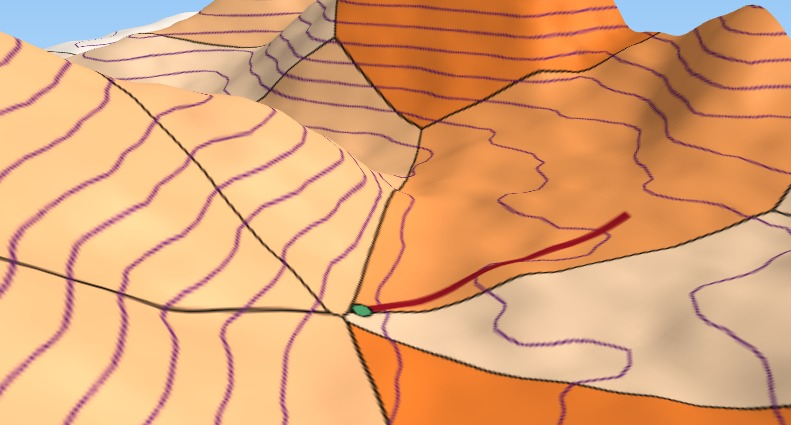
\includegraphics[width=0.45\linewidth]{img/Vigliano}} \quad
\subfloat[]
{\label{fig:aversa-b}
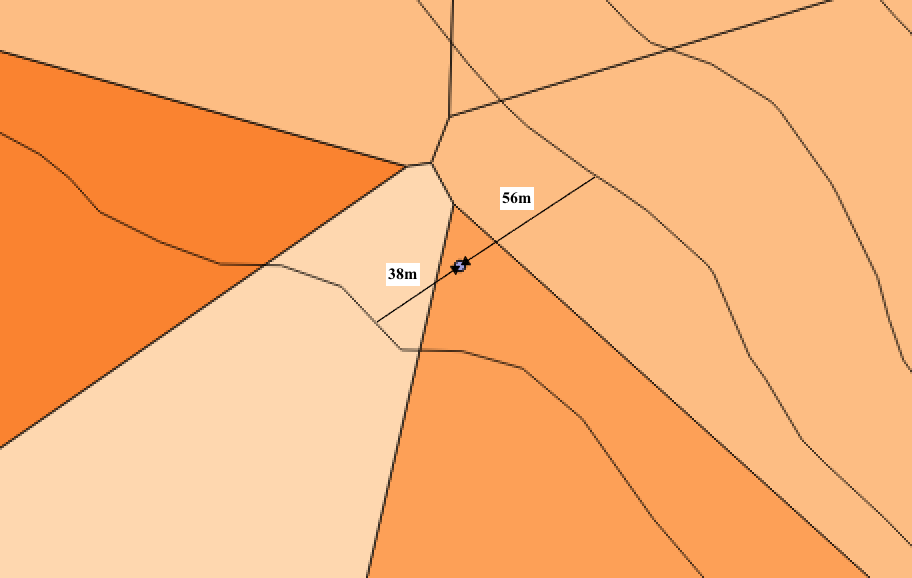
\includegraphics[width=0.38\linewidth]{img/Vigliano2}} 
\caption[]{Stazione Ferroviaria di Vigliano d'Abruzzo}\label{fig:vigliano}
\end{figure}
\end{itemize}
\newpage
\section{Ranking e Valutazione delle Linee Ferroviarie}
In questa sezione andremo a discutere i risultati ottenuti applicando il metodo NMCE presentato in Sez. \ref{metodoLinee} per la determinazione della classifica delle linee ferroviarie in relazione al grado di esposizione al rischio idrogeologico.\newline \newline
Il metodo ha restituito $690$ segmenti in quanto abbiamo definito la lunghezza di ognuno pari a $1$ km ed il valore di \textit{exposure} di ognuno varia da un valore massimo di $130$ ad un valore minimo di $0$. A fronte di tali risultati abbiamo ritenuto opportuno, per analogia al caso delle stazioni ferroviarie, utilizzare il medesimo meccanismo di classificazione in tre fasce di rischio:
\begin{itemize}
	\item High
	\item Moderate
	\item Low
\end{itemize}
La tabella \ref{rangeLinee} mostra la suddetta divisione in fasce di rischio, gli intervalli in cui i segmenti sono stati divisi secondo il valore di \textit{exposure}, il numero e la percentuale sul totale dei segmenti appartenenti ad una determinata fascia. Come nel caso delle stazioni ferroviarie ad ogni fascia abbiamo associato un colore identificativo.
\begin{table}[h]
\centering
\begin{tabular}{|c|c|c|c|}
\hline
\rowcolor{lightgray}
\textbf{Fascia} & \textbf{Intervallo valori Exp$\mathbf{\_}$$\mathbf{segmento}$} & $\mathbf{\#segmenti}$ & \textbf{\%} \\
\hline
\rowcolor{flamingopink}
High & 20 < Exp$\_$$b_i$ < 50 & 226 & 11,31\%\\
\hline
\rowcolor{icterine}
Moderate & 1 < Exp$\_$$b_i$ < 20 & 386 & 55,94\%\\
\hline
\rowcolor{inchworm}
Low & $0$ < Exp$\_$$b_i$ < 1 & 226 & 32,75\%\\
\hline
\end{tabular}
\caption{Aggregazione dei segmenti in base al valore di \textit{exposure} }
\label{rangeLinee}
\end{table}
\newline
Come è possibile notare chiaramente dai dati riportati in tabella \ref{rangeLinee} solo una bassa percentuale de segmenti presenta un livello di esposizione al rischio di frane tale da far emergere il bisogno di controlli più frequenti (livello di esposizione \textit{High}). Da tali risultati si ha quindi la conferma dell'utilità del lavoro esposto, in particolare per gli addetti al controllo della rete ferroviaria: viene ridotto al $11,31\%$ il numero di segmenti di rete ferroviaria da manutenere più frequentemente; ciò comporta senza ombra di dubbio una riduzione, in termini di costi e di tempi, per gli addetti ai lavori.\newline
In Figura \ref{rankinglinee} è possibile avere una visione d'insieme dei risultati ottenuti dall'applicazione del metodo NMCE sui segmenti delle linee che compongono la rete ferroviaria abruzzese, si noti come ogni segmento in figura ha lo stesso colore della fascia di rischio a cui appartiene.
\begin{figure}[h]
	\centering
	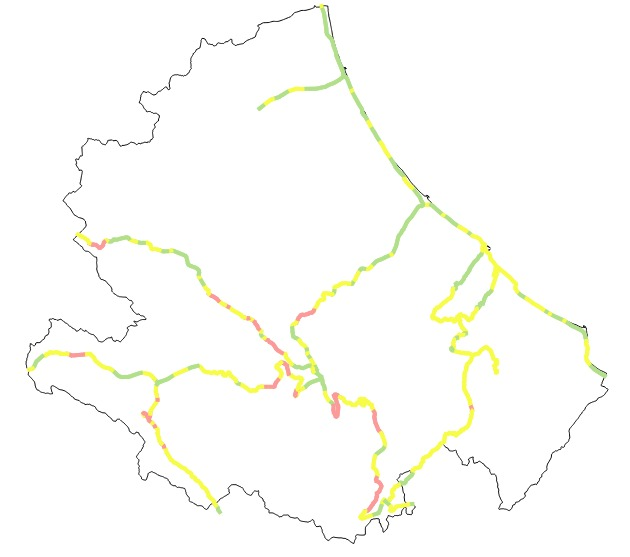
\includegraphics[width=0.4\linewidth]{img/reteRanking.jpeg}
	\caption{Visione d'insieme della classificazione in fasce di rischio dei segmenti della rete ferroviaria abruzzese}
	\label{rankinglinee}
\end{figure}
\newpage
La classifica riportata in tabella \ref{top20segmenti} mostra i primi venti (di $690$) segmenti ordinati in maniera decrescente rispetto il relativo valore di \textit{exposure}. In riferimento al singolo segmento, per ognuno di essi vengono mostrati la linea di appartenenza, il numero del segmento e il relativo valore di \textit{exposure}.
\begin{table}[h]
\centering
\begin{tabular}{|c|c|c|c|}
\hline
\rowcolor{lightgray}
n. & Linea Ferroviaria          & \# Segmento & Valore di Exp. del Segmento \\ \hline \rowcolor{flamingopink}
1  & Sulmona - L'Aquila - Rieti & $15$        & $130,14$                    \\ \hline \rowcolor{flamingopink}
2  & Sulmona - L'Aquila - Rieti & $14$        & $107,79$                    \\ \hline \rowcolor{flamingopink}
3  & Sulmona - L'Aquila - Rieti & $17$        & $103,77$                    \\ \hline \rowcolor{flamingopink}
4  & Sulmona - L'Aquila - Rieti & $16$        & $93,95$                     \\ \hline \rowcolor{flamingopink}
5  & Sulmona - Carpinone        & $57$        & $82,19$                     \\ \hline \rowcolor{flamingopink}
6  & Pescara - Roma             & $47$        & $76,54$                     \\ \hline \rowcolor{flamingopink}
7  & Pescara - Roma             & $46$        & $74,56$                     \\ \hline \rowcolor{flamingopink}
8  & Sulmona - L'Aquila - Rieti & $13$        & $71,89$                     \\ \hline \rowcolor{flamingopink}
9  & Sulmona - Carpinone        & $10$        & $64,49$                     \\ \hline \rowcolor{flamingopink}
10 & Pescara - Roma             & $158$       & $62,02$                     \\ \hline \rowcolor{flamingopink}
11 & Sulmona - Carpinone        & $58$        & $61,57$                     \\ \hline \rowcolor{flamingopink}
12 & Pescara - Roma             & $78$        & $59,00$                     \\ \hline \rowcolor{flamingopink}
13 & Sulmona - Carpinone        & $56$        & $55,16$                     \\ \hline \rowcolor{flamingopink}
14 & Sulmona - L'Aquila - Rieti & $37$        & $53,91$                     \\ \hline \rowcolor{flamingopink}
15 & Pescara - Roma             & $50$        & $51,42$                     \\ \hline \rowcolor{flamingopink}
16 & Roccasecca - Avezzano      & $35$        & $50,76$                     \\ \hline \rowcolor{flamingopink}
17 & Sulmona - L'Aquila - Rieti & $23$        & $49,65$                     \\ \hline \rowcolor{flamingopink}
18 & Sulmona - Carpinone        & $62$        & $48,71$                     \\ \hline \rowcolor{flamingopink}
19 & Sulmona - Carpinone        & $36$        & $48,04$                     \\ \hline \rowcolor{flamingopink}
20 & Sulmona - Carpinone        & $41$        & $47,93$                     \\ \hline 
\end{tabular}
\caption{Classifica generale dei primi venti (di $690$) segmenti con relativo valore di \textit{exposure} e linea di appartenenza}
\label{top20segmenti}
\end{table} 
\newpage
Si espone qui di seguito un'analisi puntuale dei risultati per ogni linea ferroviaria.

\subsection{Linea Bologna - Bari}
Si riportano in Tabella \ref{classificabolognabari} i primi dieci (di 125) segmenti di tale tratta ferroviaria ordinati in maniera decrescente rispetto il valore di \textit{exposure}.
\begin{table}[h]
\centering
\begin{tabular}{|c|c|c|}
\hline
\rowcolor{lightgray}
n. & \# Segmento & Valore di Exp. del Segmento \\ \hline \rowcolor{icterine}
1  & $41$        & $8,59$                      \\ \hline \rowcolor{icterine}
2  & $90$        & $6,43$                      \\ \hline \rowcolor{icterine}
3  & $40$        & $6,07$                      \\ \hline \rowcolor{icterine}
4  & $53$        & $5,05$                      \\ \hline \rowcolor{icterine}
5  & $42$        & $4,84$                      \\ \hline \rowcolor{icterine}
6  & $91$        & $4,82$                      \\ \hline \rowcolor{icterine}
7  & $116$       & $4,78$                      \\ \hline \rowcolor{icterine}
8  & $84$        & $4,70$                      \\ \hline \rowcolor{icterine}
9  & $85$        & $4,57$                      \\ \hline \rowcolor{icterine}
10 & $86$        & $4,27$                      \\ \hline
\end{tabular}
\caption{Classifica dei primi dieci (di 125) segmenti appartenenti alla linea Bologna - Bari}
\label{classificabolognabari}
\end{table}
\newline
La Figura \ref{bolognabari} mostra invece una visione d'insieme della classificazione in fasce di rischio dei segmenti che compongono la linea.
\begin{figure}[h]
\centering
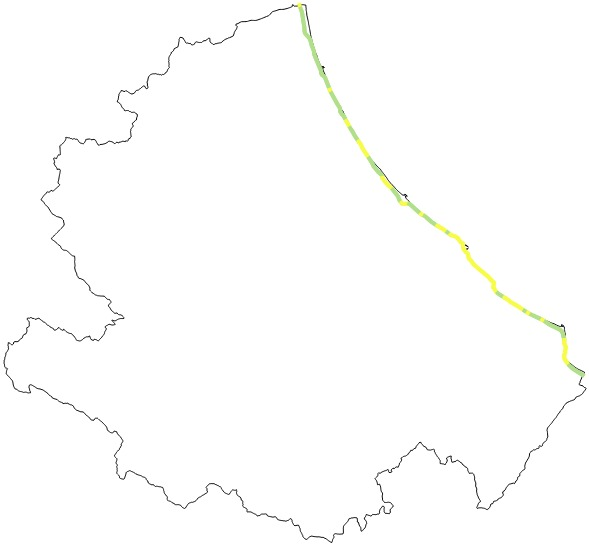
\includegraphics[width=0.4\linewidth]{img/bolognabari.jpeg}
\caption{Visione d'insieme della classificazione in fasce di rischio dei segmenti della linea Bologna - Bari}
\label{bolognabari}
\end{figure}
\newline
Analizzando i risultati esposti in Tabella \ref{percentualebolognabari} si evince che in questa linea non ci sono segmenti che destano preoccupazione circa il rischio di smottamenti. 
Per una visione completa della classificazione dei segmenti della linea Bologna - Bari si rimanda alla lettura dell'appendice \ref{app:bolognabari}.
\begin{table}[h]
\centering
\begin{tabular}{|c|c|c|}
\hline \rowcolor{lightgray}
Fascia   & \# Segmenti & \%    \\ \hline \rowcolor{flamingopink}
High     & $0$           & $0$     \\ \hline \rowcolor{icterine}
Moderate & $54$          & $43,20$ \\ \hline \rowcolor{inchworm}
Low      & $71$          & $56,80$ \\ \hline
\end{tabular}
\caption{Analisi statistica della classificazione in fasce di rischio dei segmenti della linea Bologna - Bari}
\label{percentualebolognabari}
\end{table}

\newpage
\subsection{Linea Ortona - Crocetta}
Si riportano in Tabella \ref{classificaortonacrocetta} i primi dieci (di 36) segmenti di tale tratta ferroviaria ordinati in maniera decrescente rispetto il valore di \textit{exposure}.
\begin{table}[h]
\centering
\begin{tabular}{|c|c|c|}
\hline
\rowcolor{lightgray}
n. & \# Segmento & Valore di Exp. del Segmento \\ \hline \rowcolor{icterine}
1  & $23$        & $10,22$                      \\ \hline \rowcolor{icterine}
2  & $22$        & $9,38$                      \\ \hline \rowcolor{icterine}
3  & $32$        & $5,38$                      \\ \hline \rowcolor{icterine}
4  & $25$        & $5,31$                      \\ \hline \rowcolor{icterine}
5  & $24$        & $5,18$                      \\ \hline \rowcolor{icterine}
6  & $31$        & $5,10$                      \\ \hline \rowcolor{icterine}
7  & $33$       & $5,01$                      \\ \hline \rowcolor{icterine}
8  & $36$        & $4,39$                      \\ \hline \rowcolor{icterine}
9  & $35$        & $4,13$                      \\ \hline \rowcolor{icterine}
10 & $27$        & $3,92$                      \\ \hline
\end{tabular}
\caption{Classifica dei primi dieci (di 36) segmenti appartenenti alla linea Ortona - Crocetta}
\label{classificaortonacrocetta}
\end{table}
\newline
La Figura \ref{ortonacrocetta} mostra invece una visione d'insieme della classificazione in fasce di rischio dei segmenti che compongono la linea.
\begin{figure}[h]
\centering
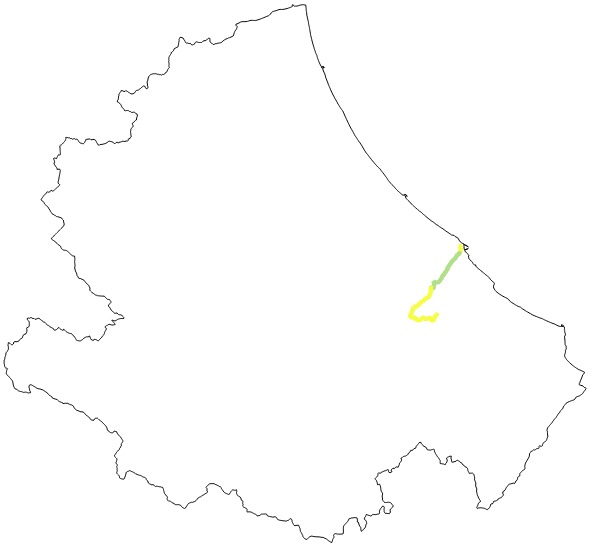
\includegraphics[width=0.4\linewidth]{img/ortonacrocetta.jpeg}
\caption{Visione d'insieme della classificazione in fasce di rischio dei segmenti della linea Ortona - Crocetta}
\label{ortonacrocetta}
\end{figure}
\newline
Analizzando i risultati esposti in Tabella \ref{percentualeortonacrocetta} si evince che in questa linea non ci sono segmenti che destano preoccupazione circa il rischio di smottamenti. 
Per una visione completa della classificazione dei segmenti della linea Ortona - Crocetta si rimanda alla lettura dell'appendice \ref{app:ortonacrocetta}.
\begin{table}[h]
\centering
\begin{tabular}{|c|c|c|}
\hline \rowcolor{lightgray}
Fascia   & \# Segmenti & \%    \\ \hline \rowcolor{flamingopink}
High     & $0$           & $0$     \\ \hline \rowcolor{icterine}
Moderate & $54$          & $43,20$ \\ \hline \rowcolor{inchworm}
Low      & $71$          & $56,80$ \\ \hline
\end{tabular}
\caption{Analisi statistica della classificazione in fasce di rischio dei segmenti della linea Ortona - Crocetta}
\label{percentualeortonacrocetta}
\end{table}
\newpage
\subsection{Linea Marina di San Vito - Castel di Sangro}
Si riportano in Tabella \ref{classificamarinadisanvitocasteldisangro} i primi dieci (di 125) segmenti di tale tratta ferroviaria ordinati in maniera decrescente rispetto il valore di \textit{exposure}.
\begin{table}[h]
\centering
\begin{tabular}{|c|c|c|}
\hline
\rowcolor{lightgray}
n. & \# Segmento & Valore di Exp. del Segmento \\ \hline \rowcolor{flamingopink}
1  & $64$        & $20,43$                      \\ \hline \rowcolor{icterine}
2  & $78$        & $17,92$                      \\ \hline \rowcolor{icterine}
3  & $79$        & $17,10$                      \\ \hline \rowcolor{icterine}
4  & $73$        & $17,04$                      \\ \hline \rowcolor{icterine}
5  & $68$        & $15,80$                      \\ \hline \rowcolor{icterine}
6  & $76$        & $15,55$                      \\ \hline \rowcolor{icterine}
7  & $56$       & $15,54$                      \\ \hline \rowcolor{icterine}
8  & $77$        & $14,32$                      \\ \hline \rowcolor{icterine}
9  & $70$        & $14,28$                      \\ \hline \rowcolor{icterine}
10 & $75$        & $13,91$                      \\ \hline
\end{tabular}
\caption{Classifica dei primi dieci (di 105) segmenti appartenenti alla linea Marina di San Vito - Castel di Sangro}
\label{classificamarinadisanvitocasteldisangro}
\end{table}
\newline
La Figura \ref{sanvitocasteldisangro} mostra invece una visione d'insieme della classificazione in fasce di rischio dei segmenti che compongono la linea.
\begin{figure}[h]
\centering
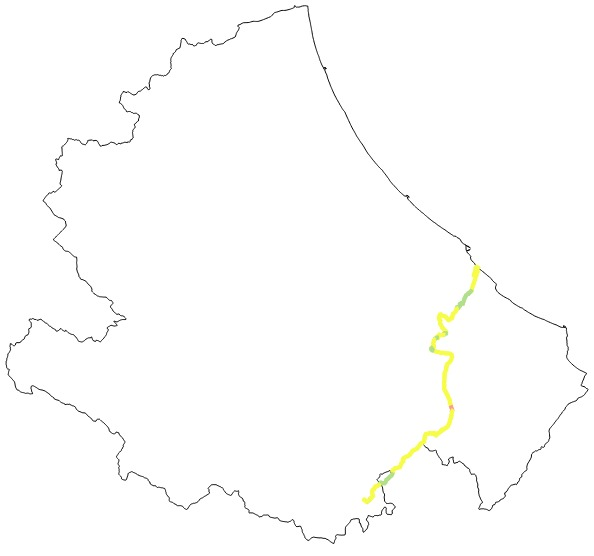
\includegraphics[width=0.4\linewidth]{img/sanvitocasteldisangro.jpeg}
\caption{Visione d'insieme della classificazione in fasce di rischio dei segmenti della linea Marina di San Vito - Castel di Sangro}
\label{sanvitocasteldisangro}
\end{figure}
\newline
Analizzando i risultati esposti in Tabella \ref{percentualesanvitocasteldisangro} si evince che in questa linea solo il $0,95\%$ dei segmenti si trova in fascia \textit{High} e quindi deve essere sottoposto a controlli più frequenti vista la sua esposizione al rischio idrogeologico. 
Per una visione completa della classificazione dei segmenti della linea Marina di San Vito - Castel di Sangro si rimanda alla lettura dell'appendice \ref{app:sanvitocasteldisangro}.
\begin{table}[h]
\centering
\begin{tabular}{|c|c|c|}
\hline \rowcolor{lightgray}
Fascia   & \# Segmenti & \%    \\ \hline \rowcolor{flamingopink}
High     & $1$           & $0,95$     \\ \hline \rowcolor{icterine}
Moderate & $87$          & $82,86$ \\ \hline \rowcolor{inchworm}
Low      & $17$          & $16,19$ \\ \hline
\end{tabular}
\caption{Analisi statistica della classificazione in fasce di rischio dei segmenti della linea Marina di San Vito - Castel di Sangro}
\label{percentualesanvitocasteldisangro}
\end{table}
\newpage
\subsection{Linea Pescara - Roma}
Si riportano in Tabella \ref{classificapescararoma} i primi dieci (di 170) segmenti di tale tratta ferroviaria ordinati in maniera decrescente rispetto il valore di \textit{exposure}.
\begin{table}[h]
\centering
\begin{tabular}{|c|c|c|}
\hline
\rowcolor{lightgray}
n. & \# Segmento & Valore di Exp. del Segmento \\ \hline \rowcolor{flamingopink}
1  & $47$        & $76,54$                      \\ \hline \rowcolor{flamingopink}
2  & $46$        & $74,56$                      \\ \hline \rowcolor{flamingopink}
3  & $158$        & $62,02$                      \\ \hline \rowcolor{flamingopink}
4  & $78$        & $59,00$                      \\ \hline \rowcolor{flamingopink}
5  & $50$        & $46,78$                      \\ \hline \rowcolor{flamingopink}
6  & $88$        & $45,87$                      \\ \hline \rowcolor{flamingopink}
7  & $157$       & $45,87$                      \\ \hline \rowcolor{flamingopink}
8  & $48$        & $45,59$                      \\ \hline \rowcolor{flamingopink}
9  & $98$        & $38,57$                      \\ \hline \rowcolor{flamingopink}
10 & $89$        & $36,85$                      \\ \hline
\end{tabular}
\caption{Classifica dei primi dieci (di 170) segmenti appartenenti alla linea Pescara - Roma}
\label{classificapescararoma}
\end{table}
\newline
La Figura \ref{pescararoma} mostra invece una visione d'insieme della classificazione in fasce di rischio dei segmenti che compongono la linea.
\begin{figure}[h]
\centering
\includegraphics[width=0.4\linewidth]{img/romapescara.jpeg}
\caption{Visione d'insieme della classificazione in fasce di rischio dei segmenti della linea Pescara - Roma}
\label{pescararoma}
\end{figure}
\newline
Analizzando i risultati esposti in Tabella \ref{percentualepescararoma} si evince che in questa linea solo il $12,94\%$ dei segmenti si trova in fascia \textit{High} e quindi deve essere sottoposto a controlli più frequenti vista la sua esposizione al rischio idrogeologico. 
Per una visione completa della classificazione dei segmenti della linea Pescara - Roma si rimanda alla lettura dell'appendice \ref{app:pescararoma}.
\begin{table}[h]
\centering
\begin{tabular}{|c|c|c|}
\hline \rowcolor{lightgray}
Fascia   & \# Segmenti & \%    \\ \hline \rowcolor{flamingopink}
High     & $22$           & $12,94$     \\ \hline \rowcolor{icterine}
Moderate & $87$          & $51,18$ \\ \hline \rowcolor{inchworm}
Low      & $61$          & $35,88$ \\ \hline
\end{tabular}
\caption{Analisi statistica della classificazione in fasce di rischio dei segmenti della linea Pescara - Roma}
\label{percentualepescararoma}
\end{table}
\newpage
\subsection{Linea Roccasecca - Avezzano}
Si riportano in Tabella \ref{classificaroccaseccaavezzano} i primi dieci (di 46) segmenti di tale tratta ferroviaria ordinati in maniera decrescente rispetto il valore di \textit{exposure}.
\begin{table}[h]
\centering
\begin{tabular}{|c|c|c|}
\hline
\rowcolor{lightgray}
n. & \# Segmento & Valore di Exp. del Segmento \\ \hline \rowcolor{flamingopink}
1  & $35$        & $50,76$                      \\ \hline \rowcolor{flamingopink}
2  & $42$        & $36,80$                      \\ \hline \rowcolor{flamingopink}
3  & $36$        & $34,80$                      \\ \hline \rowcolor{flamingopink}
4  & $37$        & $34,77$                      \\ \hline \rowcolor{flamingopink}
5  & $32$        & $27,77$                      \\ \hline \rowcolor{flamingopink}
6  & $24$        & $25,48$                      \\ \hline \rowcolor{flamingopink}
7  & $33$       & $24,48$                      \\ \hline \rowcolor{flamingopink}
8  & $30$        & $20,27$                      \\ \hline \rowcolor{icterine}
9  & $43$        & $19,46$                      \\ \hline \rowcolor{icterine}
10 & $34$        & $19,14$                      \\ \hline
\end{tabular}
\caption{Classifica dei primi dieci (di 46) segmenti appartenenti alla linea Roccasecca - Avezzano}
\label{classificaroccaseccaavezzano}
\end{table}
\newline
La Figura \ref{avezzanoroccasecca} mostra invece una visione d'insieme della classificazione in fasce di rischio dei segmenti che compongono la linea.
\begin{figure}[h]
\centering
\includegraphics[width=0.4\linewidth]{img/avezzanoroccasecca.jpeg}
\caption{Visione d'insieme della classificazione in fasce di rischio dei segmenti della linea Roccasecca - Avezzano}
\label{avezzanoroccasecca}
\end{figure}
\newline
Analizzando i risultati esposti in Tabella \ref{percentualeavezzanoroccasecca} si evince che in questa linea solo il $17,39\%$ dei segmenti si trova in fascia \textit{High} e quindi deve essere sottoposto a controlli più frequenti vista la sua esposizione al rischio idrogeologico. 
Per una visione completa della classificazione dei segmenti della linea Roccasecca - Avezzano si rimanda alla lettura dell'appendice \ref{app:avezzanoroccasecca}.
\begin{table}[h]
\centering
\begin{tabular}{|c|c|c|}
\hline \rowcolor{lightgray}
Fascia   & \# Segmenti & \%    \\ \hline \rowcolor{flamingopink}
High     & $8$           & $17,39$     \\ \hline \rowcolor{icterine}
Moderate & $35$          & $76,09$ \\ \hline \rowcolor{inchworm}
Low      & $3$          & $6,52$ \\ \hline
\end{tabular}
\caption{Analisi statistica della classificazione in fasce di rischio dei segmenti della linea Roccasecca - Avezzano}
\label{percentualeavezzanoroccasecca}
\end{table}
\newpage
\subsection{Linea Archi Stazione - Atessa}
Si riportano in Tabella \ref{classificaarchiatessa} i primi dieci (di 15) segmenti di tale tratta ferroviaria ordinati in maniera decrescente rispetto il valore di \textit{exposure}.
\begin{table}[h]
\centering
\begin{tabular}{|c|c|c|}
\hline
\rowcolor{lightgray}
n. & \# Segmento & Valore di Exp. del Segmento \\ \hline \rowcolor{icterine}
1  & $14$        & $4,63$                      \\ \hline \rowcolor{icterine}
2  & $15$        & $4,20$                      \\ \hline \rowcolor{icterine}
3  & $2$        & $3,75$                      \\ \hline \rowcolor{icterine}
4  & $13$        & $3,39$                      \\ \hline \rowcolor{icterine}
5  & $3$        & $2,47$                      \\ \hline \rowcolor{icterine}
6  & $12$        & $2,39$                      \\ \hline \rowcolor{icterine}
7  & $1$       & $2,04$                      \\ \hline \rowcolor{icterine}
8  & $11$        & $1,85$                      \\ \hline \rowcolor{icterine}
9  & $10$        & $1,70$                      \\ \hline \rowcolor{icterine}
10 & $7$        & $1,53$                      \\ \hline
\end{tabular}
\caption{Classifica dei primi dieci (di 15) segmenti appartenenti alla linea Archi Stazione - Atessa}
\label{classificaarchiatessa}
\end{table}
\newline
La Figura \ref{archiatessa} mostra invece una visione d'insieme della classificazione in fasce di rischio dei segmenti che compongono la linea.
\begin{figure}[h]
\centering
\includegraphics[width=0.4\linewidth]{img/archiatessa.jpeg}
\caption{Visione d'insieme della classificazione in fasce di rischio dei segmenti della linea Archi Stazione - Atessa}
\label{archiatessa}
\end{figure}
\newline
Analizzando i risultati esposti in Tabella \ref{percentualearchiatessa} si evince che in questa linea non ci sono segmenti che destano preoccupazione circa il rischio di smottamenti. 
Per una visione completa della classificazione dei segmenti della linea Archi Stazione - Atessa si rimanda alla lettura dell'appendice \ref{app:archiatessa}.
\begin{table}[h]
\centering
\begin{tabular}{|c|c|c|}
\hline \rowcolor{lightgray}
Fascia   & \# Segmenti & \%    \\ \hline \rowcolor{flamingopink}
High     & $0$           & $0$     \\ \hline \rowcolor{icterine}
Moderate & $15$          & $100$ \\ \hline \rowcolor{inchworm}
Low      & $0$          & $0$ \\ \hline
\end{tabular}
\caption{Analisi statistica della classificazione in fasce di rischio dei segmenti della linea Archi Stazione - Atessa}
\label{percentualearchiatessa}
\end{table}
\newpage
\subsection{Linea Sulmona - Carpinone}
Si riportano in Tabella \ref{classificasulmonacarpinone} i primi dieci (di 86) segmenti di tale tratta ferroviaria ordinati in maniera decrescente rispetto il valore di \textit{exposure}.
\begin{table}[h]
\centering
\begin{tabular}{|c|c|c|}
\hline
\rowcolor{lightgray}
n. & \# Segmento & Valore di Exp. del Segmento \\ \hline \rowcolor{flamingopink}
1  & $57$        & $82,19$                      \\ \hline \rowcolor{flamingopink}
2  & $10$        & $64,49$                      \\ \hline \rowcolor{flamingopink}
3  & $58$        & $61,57$                      \\ \hline \rowcolor{flamingopink}
4  & $56$        & $55,16$                      \\ \hline \rowcolor{flamingopink}
5  & $62$        & $48,71$                      \\ \hline \rowcolor{flamingopink}
6  & $36$        & $48,04$                      \\ \hline \rowcolor{flamingopink}
7  & $42$       & $47,93$                      \\ \hline \rowcolor{flamingopink}
8  & $18$        & $42,72$                      \\ \hline \rowcolor{flamingopink}
9  & $12$        & $41,53$                      \\ \hline \rowcolor{flamingopink}
10 & $19$        & $39,95$                      \\ \hline
\end{tabular}
\caption{Classifica dei primi dieci (di 86) segmenti appartenenti alla linea Sulmona - Carpinone}
\label{classificasulmonacarpinone}
\end{table}
\newline
La Figura \ref{sulmonacarpinone} mostra invece una visione d'insieme della classificazione in fasce di rischio dei segmenti che compongono la linea.
\begin{figure}[h]
\centering
\includegraphics[width=0.4\linewidth]{img/sulmonacarpinone.jpeg}
\caption{Visione d'insieme della classificazione in fasce di rischio dei segmenti della linea Sulmona - Carpinone}
\label{sulmonacarpinone}
\end{figure}
\newline
Analizzando i risultati esposti in Tabella \ref{percentualesulmonacarpinone} si evince che in questa linea solo il $32,56\%$ dei segmenti si trova in fascia \textit{High} e quindi deve essere sottoposto a controlli più frequenti vista la sua esposizione al rischio idrogeologico. 
Per una visione completa della classificazione dei segmenti della linea Sulmona - Carpinone si rimanda alla lettura dell'appendice \ref{app:sulmonacarpinone}.
\begin{table}[h]
\centering
\begin{tabular}{|c|c|c|}
\hline \rowcolor{lightgray}
Fascia   & \# Segmenti & \%    \\ \hline \rowcolor{flamingopink}
High     & $28$           & $32,56$     \\ \hline \rowcolor{icterine}
Moderate & $44$          & $51,16$ \\ \hline \rowcolor{inchworm}
Low      & $14$          & $16,28$ \\ \hline
\end{tabular}
\caption{Analisi statistica della classificazione in fasce di rischio dei segmenti della linea Sulmona - Carpinone}
\label{percentualesulmonacarpinone}
\end{table}
\newpage
\subsection{Linea Sulmona - L'Aquila - Rieti}
Si riportano in Tabella \ref{classificasulmonarieti} i primi dieci (di 81) segmenti di tale tratta ferroviaria ordinati in maniera decrescente rispetto il valore di \textit{exposure}.
\begin{table}[h]
\centering
\begin{tabular}{|c|c|c|}
\hline
\rowcolor{lightgray}
n. & \# Segmento & Valore di Exp. del Segmento \\ \hline \rowcolor{flamingopink}
1  & $56$        & $130,14$                      \\ \hline \rowcolor{flamingopink}
2  & $55$        & $107,79$                      \\ \hline \rowcolor{flamingopink}
3  & $63$        & $103,77$                      \\ \hline \rowcolor{flamingopink}
4  & $62$        & $93,95$                      \\ \hline \rowcolor{flamingopink}
5  & $53$        & $71,89$                      \\ \hline \rowcolor{flamingopink}
6  & $42$        & $53,91$                      \\ \hline \rowcolor{flamingopink}
7  & $71$       & $49,65$                      \\ \hline \rowcolor{flamingopink}
8  & $40$        & $44,97$                      \\ \hline \rowcolor{flamingopink}
9  & $70$        & $40,37$                      \\ \hline \rowcolor{flamingopink}
10 & $32$        & $39,55$                      \\ \hline
\end{tabular}
\caption{Classifica dei primi dieci (di 81) segmenti appartenenti alla linea Sulmona - L'Aquila - Rieti}
\label{classificasulmonarieti}
\end{table}
\newline
La Figura \ref{sulmonarieti} mostra invece una visione d'insieme della classificazione in fasce di rischio dei segmenti che compongono la linea. Questa è la tratta che tra tutte presenta i valori di \textit{exposure} dei segmenti più alti. 
\begin{figure}[h]
\centering
\includegraphics[width=0.4\linewidth]{img/rietisulmona.jpeg}
\caption{Visione d'insieme della classificazione in fasce di rischio dei segmenti della linea Sulmona - L'Aquila - Rieti}
\label{sulmonacarpinone}
\end{figure}
\newline
Analizzando i risultati esposti in Tabella \ref{percentualesulmonarieti} si evince che in questa linea solo il $23,46\%$ dei segmenti si trova in fascia \textit{High} e quindi deve essere sottoposto a controlli più frequenti vista la sua esposizione al rischio idrogeologico. Per una visione completa della classificazione dei segmenti della linea Sulmona - L'Aquila - Rieti si rimanda alla lettura dell'appendice \ref{app:sulmonarieti}.
\begin{table}[h]
\centering
\begin{tabular}{|c|c|c|}
\hline \rowcolor{lightgray}
Fascia   & \# Segmenti & \%    \\ \hline \rowcolor{flamingopink}
High     & $19$           & $23,46$     \\ \hline \rowcolor{icterine}
Moderate & $33$          & $40,74$ \\ \hline \rowcolor{inchworm}
Low      & $29$          & $35,80$ \\ \hline
\end{tabular}
\caption{Analisi statistica della classificazione in fasce di rischio dei segmenti della linea Sulmona - L'Aquila - Rieti}
\label{percentualesulmonarieti}
\end{table}
\newpage
\subsection{Linea Giulianova - Teramo}
Si riportano in Tabella \ref{classificagiulianovateramo} i primi dieci (di 26) segmenti di tale tratta ferroviaria ordinati in maniera decrescente rispetto il valore di \textit{exposure}.
\begin{table}[h]
\centering
\begin{tabular}{|c|c|c|}
\hline
\rowcolor{lightgray}
n. & \# Segmento & Valore di Exp. del Segmento \\ \hline \rowcolor{icterine}
1  & $17$        & $2,99$                      \\ \hline \rowcolor{icterine}
2  & $14$        & $2,19$                      \\ \hline \rowcolor{icterine}
3  & $23$        & $2,15$                      \\ \hline \rowcolor{icterine}
4  & $13$        & $1,96$                      \\ \hline \rowcolor{icterine}
5  & $16$        & $1,72$                      \\ \hline \rowcolor{icterine}
6  & $15$        & $1,40$                      \\ \hline \rowcolor{icterine}
7  & $22$       & $1,24$                      \\ \hline \rowcolor{icterine}
8  & $24$        & $1,12$                      \\ \hline \rowcolor{inchworm}
9  & $25$        & $0,80$                      \\ \hline \rowcolor{inchworm}
10 & $12$        & $0,72$                      \\ \hline
\end{tabular}
\caption{Classifica dei primi dieci (di 26) segmenti appartenenti alla linea Giulianova - Teramo}
\label{classificagiulianovateramo}
\end{table}
\newline
La Figura \ref{giulianovateramo} mostra invece una visione d'insieme della classificazione in fasce di rischio dei segmenti che compongono la linea.
\begin{figure}[h]
\centering
\includegraphics[width=0.4\linewidth]{img/teramogiulianova.jpeg}
\caption{Visione d'insieme della classificazione in fasce di rischio dei segmenti della linea Giulianova - Teramo}
\label{giulianovateramo}
\end{figure}
\newline
Analizzando i risultati esposti in Tabella \ref{percentualegiulianovateramo} si evince che in questa linea non ci sono segmenti che destano preoccupazione circa il rischio di smottamenti. 
Per una visione completa della classificazione dei segmenti della linea Giulianova - Teramo si rimanda alla lettura dell'appendice \ref{app:giulianovateramo}.
\begin{table}[h]
\centering
\begin{tabular}{|c|c|c|}
\hline \rowcolor{lightgray}
Fascia   & \# Segmenti & \%    \\ \hline \rowcolor{flamingopink}
High     & $0$           & $0$     \\ \hline \rowcolor{icterine}
Moderate & $8$          & $30,77$ \\ \hline \rowcolor{inchworm}
Low      & $18$          & $69,23,$ \\ \hline
\end{tabular}
\caption{Analisi statistica della classificazione in fasce di rischio dei segmenti della linea Giulianova - Teramo}
\label{percentualegiulianovateramo}
\end{table}
\newpage
\subsection{Discussione dei risultati ottenuti}
Per la validazione dei risultati ottenuti dall'applicazione del metodo NMCE, discusso nella Sezione \ref{metodoLinee}, sono stati utilizzati il software QGIS, presentato in appendice \ref{qgis}, e GoogleMaps, con lo scopo di verificare, almeno dal punto di vista visivo, la classificazione in fasce di rischio ottenuta. 
 Un ulteriore controllo è stato realizzato confrontando la fascia di rischio associata al segmento della linea ferroviaria e la fascia di rischio associata alla stazione che insiste su di esso: In alcuni casi la fascia del segmento è in contrasto con la fascia assegnata alla stazione ferroviaria dal NMC. Questi casi corrispondono ai casi critici di cui abbiamo ampiamente parlato nella sezione \ref{discussioneRisultati}. Ad esempio la stazione di Aversa sappiamo essere stata classificata erroneamente nella fascia \textit{Moderate} dal NMC. Invece il NMCE classifica i segmenti in prossimità della stazione nella fascia \textit{High} come si evince dalla Fig.\ref{aversalinea}
\begin{figure}[bth]
\myfloatalign
\subfloat[]
{\includegraphics[width=0.4\linewidth]{img/aversaLinea}} \quad
\subfloat[]
{\includegraphics[width=0.4\linewidth]{img/AversaLinea3}} 
\caption{Vista $2$D (a) e $3$D (b) della stazione di Aversa e della linea ferroviaria che l’attraversa}\label{aversalinea}

\end{figure}
\newline
Il metodo NMCE presenta inoltre una criticità che determina in alcuni casi la presenza di \textit{falsi positivi}: L'assenza di un dataset che informi circa la presenza di gallerie ferroviarie: Il metodo, non avendo conoscenza della loro presenza o meno, non riesce ad individuare le situazioni in cui i binari della linea ferroviaria proseguono all'interno di una galleria e crede che la tratta prosegui arrampicandosi sul il pendio, generando così valori di \textit{exposure} errati.
In Figura \ref{} è possibile osservare una di queste situazioni critiche, corrispondenti alla tratta ferroviaria Pescara - Roma, dal km $154$ al km $157$, mentre in Figura \ref{esempiogalleria} è possibile osservare la stessa tratta fotografata tramite GoogleMaps.
\begin{figure}[bth]
\myfloatalign
\subfloat[]
{\includegraphics[width=0.4\linewidth]{img/esempioGalleria2}} \quad
\subfloat[]
{\includegraphics[width=0.4\linewidth]{img/esempioGalleria3}} 
\caption{ Vista $2$D (a) e $3$D (b) della tratta Pescara - Roma dal km $154$ al $157$}
\label{esempiogalleria}
\end{figure}

%inserire immagine googlemaps e revisionare paginazione
\chapter{Considerazioni finali e proposte per lavori futuri}
\label{ch:conclusionilavorifuturi}

In questo capitolo andremo a riportare alcune considerazioni circa i metodi discussi per il ranking delle tratte ferroviarie e delle stazioni che su di esse insistono al fine di proporre spunti per i lavori futuri. Inoltre verranno evidenziate alcune inesattezze riscontrate nei dataset utilizzati.
\newline
In conclusione è presente un riepilogo del lavoro svolto.
\section{Proposte per lavori futuri sul metodo di ranking delle stazioni ferroviarie}
Benchè il metodo di ranking delle stazioni ferroviarie di cui abbiamo discusso nella sezione \ref{metodoNuovo} abbia consentito il raggiungimento dell'obiettivo preposto per tale laboratorio (esposto nel Cap. \ref{ch:introduzione}) è opportuno comunque fare alcune considerazioni a riguardo, al fine di ottenere degli spunti per eventuali lavori futuri. Come abbiamo già discusso nella sezione \ref{discussioneRisultati}, il metodo NMC ha buone performance e riesce generalmente ad individuare quali sono le stazioni ferroviarie che necessitano di un monitoraggio più frequente da parte degli organi competenti data la loro esposizione al rischio di frane ma presenta alcune limitazioni che ci hanno consentito di realizzare alcune considerazioni a partire dalle quali abbiamo ipotizzato alcuni spunti operativi per lavori futuri. Uno tra questi consiste nell'idea di poter considerare nell'intorno del punto \textit{$b_i$} che individua l'edificio della stazione ferroviaria un triangolo in cui \textit{$b_i$} rappresenta il baricentro (vedi Fig. \ref{baricentro}).
\begin{figure}[hpt]
	\centering
	\includegraphics[width=0.5\linewidth]{img/baricentro}
	\caption{Triangolo costruito nell'intorno di \textit{$b_i$}}
	\label{baricentro}
\end{figure}

Sui vertici di tale figura sarà possibile calcolare il valore di \textit{exposure} corrispondente così come esposto nella Sez. \ref{metodoNuovo}: Il valore di \textit{exposure} associato alla stazione ferroviaria \textit{$b_i$} sarà pari alla loro media aritmetica.
Così facendo, considerando più punti nell'intorno dell'edificio sarà possibile ottenere valori di \textit{exposure} più coerenti con la reale conformazione morfologica del terreno circostante, superando di conseguenza le limitazioni di cui abbiamo discusso nella Sez. \ref{discussioneRisultati}.
 
\section{Proposte per lavori futuri sul metodo di ranking delle tratte ferroviarie}
Il metodo NMCE, discusso nella Sez. \ref{metodoLinee}, proposto per il ranking delle tratte ferroviarie circa il loro livello di esposizione al rischio di frane ci ha consentito di realizzare una valutazione circa le loro potenziali pericolosità. Uno spunto per dei lavori futuri al fine di migliorare l'affidabilità dei risultati ottenuti potrebbe essere quello di introdurre dei dataset circa le gallerie e i ponti ferroviari dislocati lungo la rete ferroviaria. Questi infatti sono nel nostro metodo NMCE fonte di falsi positivi nella classificazione in fasce di rischio dei segmenti della rete ferroviaria, come abbiamo già discusso nella Sez. \ref{discussioneLinee}.
\section{Considerazioni sui dataset}
Nella valutazione delle performance dei metodi proposti non è possibile prescindere dalla consapevolezza che i dataset utilizzati potrebbero essere incompleti o potrebbero presentare imprecisioni. 
Uno spunto per dei lavori futuri potrebbe essere quello di utilizzare un dataset della rete ferroviaria e delle stazioni che insistono su di essa aggiornato, tale da limitare le inesattezze dei risultati. Infatti, in seguito ad accurate ricerche effettuate in rete, risulta evidente che alcune tratte, nonchè alcune stazioni situate lungo di esse, sono inattive o in fase di smantellamento. I portali che abbiamo utilizzato maggiormente sono quello proposto da Trenitalia (\url{http://www.rfi.it/rfi/LINEE-STAZIONI-TERRITORIO/Nelle-regioni/Abruzzo/La-rete-oggi-in:-Abruzzo}) e \url{http://www.ferrovieabbandonate.it/}.
\newpage
Qui di seguito alcune foto di stazioni ferroviarie ormai dismesse o in disuso: Archi (Fig. \ref{archi}) , Perano (Fig. \ref{perano}), Pettorano sul Gizio (Fig. \ref{pettorano}) e Civitaluparella (Fig. \ref{civitaluparella}).
\begin{figure}[h]
\centering
\begin{minipage}[c]{.40\textwidth}
\centering\setlength{\captionmargin}{0pt}%
\includegraphics[width=.60\textwidth]{img/archi}
\caption{Stazione di Archi}
\label{archi}
\end{minipage}%
\hspace{10mm}%
\begin{minipage}[c]{.40\textwidth}
\centering\setlength{\captionmargin}{0pt}%
\includegraphics[width=.60\textwidth]{img/perano}
\caption{Stazione di Perano}
\label{perano}
\end{minipage}
\begin{minipage}[c]{.40\textwidth}
\centering\setlength{\captionmargin}{0pt}%
\includegraphics[width=.60\textwidth]{img/pettorano}
\caption{Stazione di Pettorano}
\label{pettorano}
\end{minipage}%
\hspace{10mm}%
\begin{minipage}[c]{.40\textwidth}
\centering\setlength{\captionmargin}{0pt}%
\includegraphics[width=.60\textwidth]{img/civitaluparella}
\caption{Stazione di Civitaluparella}
\label{civitaluparella}
\end{minipage}
\end{figure}

E' necessaria inoltre un'altra riflessione circa i dataset utilizzati, quella circa il dataset delle zone in cui è stato deframmentato il territorio abruzzese. Il dataset in nostro possesso è l'output di un metodo che sfrutta un algoritmo che si basa sul \textit{Diagramma di Voronoi} per decomporre il territorio, per cui le zone ottenute potrebbero non rispecchiare in maniera coerente le caratteristiche morfologiche del terreno. Bisogna inoltre considerare che il valore numerico che quantifica la pericolosità di frana di ogni zona è strettamente legato alle curve di livello che sono presenti in tale zona e non tiene conto di quelle che sono le caratteristiche litologiche del terreno. 
Uno spunto per i lavori futuri potrebbe essere quello di utilizzare un dataset delle zone che presenti maggiore affidabilità circa la morfologia e le caratteristiche del territorio.
\section{Considerazioni finali}

L’obiettivo di questo studio è stato fornire una classifica circa le stazioni e le linee ferroviarie in base al loro livello di esposizione al rischio frane. Sono stati proposti rispettivamente due metodi al fine di raggiungere tale scopo.  Successivamente è stata progettata una base di dati spaziale atta a contenere i dataset presi in input. Nel nostro caso di studio questi ultimi hanno interessato la regione Abruzzo. La base di dati spaziale è stata implementata tramite il DBMS PostgreSQL servendoci dell’estensione spaziale PostGIS. Sono state implementate delle UDF, e definite apposite query, tramite le quali poter raggiungere l’obiettivo preposto. Dopo un’analisi dei risultati ottenuti, si è proceduto alla discussione circa le criticità dei metodi e dei dataset in input. E' opportuno sottolineare come i metodi proposti non abbiano la pretesa di restituire valori assoluti circa l’esposizione al pericolo di frane, bensì quello di fornire una metodologia valida applicabile e ovviamente migliorabile per determinare delle classifiche grazie alle quali è possibile individuare le stazioni e le tratte ferroviarie che sono maggiormente esposte al pericolo di smottamenti. I risultati finali sono migliorabili sulla base degli spunti offerti durante la trattazione.  
\cleardoublepage

%----------------------------------------------------------------------------------------
%	Appendici della relazione
%----------------------------------------------------------------------------------------

\appendix

\part{Appendici}

\chapter{Appendice A}
\label{appendiceA}
\section{Proposta alternativa di Dataset delle Zone}
\label{nostraProposta}
Prima di approdare al dataset delle zone di cui abbiamo discusso nella Sez. \ref{zone}, abbiamo ipotizzato e implementato un metodo in grado di restituirci un dataset delle zone in cui suddividere l'Abruzzo prendendo come punto di partenza il dataset delle zone prodotto dall'esecuzione della seguente \textit{query} su PostGreSQL:
\begin{quote}
CREATE TABLE \textit{GeoArea\_split8} (
\newline
\textit{id} serial PRIMARY KEY,
\newline
\textit{geom} geometry (Polygon, 3004))
\newline
\newline
INSERT INTO \textit{GeoArea\_split8} (geom) 
\newline
SELECT ST\_Subdivide(geom,8)
\newline
FROM \textit{Geo\_Area}
\end{quote}

L'invocazione della funzione \textbf{ST\_Subdivide()} sulla geometria che descrive \textit{GeoArea} genera $24142$ zone in cui è suddiviso il territorio abruzzese, di cui è possibile avere una visione d'insieme in Fig. \ref{nostrodataset}.
\begin{figure}[h]
\centering
\includegraphics[width=0.4\textwidth]{img/nostrodataset}
\caption{Visione d'insieme delle $24142$ zone generate}
\label{nostrodataset}
\end{figure}
\begin{figure}[h]
\centering
\includegraphics[width=0.3\textwidth]{img/bordo}
\caption{Particolare delle zone in prossimità del \textit{boundary}}
\label{bordo}
\end{figure}
L'esame della Fig. \ref{bordo} fornisce una visione più nitida del tipo di suddivisione effettuata da ST\_Subdivide(). Esso in prossimità del \textit{boundary} della \textit{GeoArea} costruisce poligoni di forma irregolare aventi al massimo otto vertici, mentre tutte le altre aree sono dei quadrati di area crescente via via che ci si sposta verso il centro della \textit{GeoArea}.
Al fine di realizzare un'analisi quantitativa dell'esito del partizionamento della \textit{GeoArea} si riportano in tabella \ref{topMax} e in tabella \ref{topMin} rispettivamente le dieci aree con area maggiore e le dieci con aree minore.

\begin{table}[h]
\centering
\begin{tabular}{|c|c|}
\hline
\rowcolor{lightgray}
Area (kmq)                  & Perimetro (km)             \\
\hline
$3,46$ $\times$ $10^{-11}$  & $3,55$ $\times$ $10^{-5}$  \\
\hline
$1,14$ $\times$ $10^{-10}$  & $5,74$ $\times$ $10^{-5}$  \\
\hline
$3,11$ $\times$ $10^{-10}$  & $8,64$ $\times$ $10^{-5}$  \\
\hline
$3,21$ $\times$ $10^{-10}$  & $8,84$ $\times$ $10^{-5}$  \\
\hline
$6,29$ $\times$ $10^{-10}$  & $19,22$ $\times$ $10^{-5}$ \\
\hline
$6,46$ $\times$ $10^{-10}$  & $14,01$ $\times$ $10^{-5}$ \\
\hline
$6,86$ $\times$ $10^{-10}$  & $14,38$ $\times$ $10^{-5}$ \\
\hline
$8,90$ $\times$ $10^{-10}$  & $16,65$ $\times$ $10^{-5}$ \\
\hline
$11,81$ $\times$ $10^{-10}$ & $19,91$ $\times$ $10^{-5}$ \\
\hline
$13,05$ $\times$ $10^{-10}$ & $17,51$ $\times$ $10^{-5}$ \\
\hline
\end{tabular}
\caption{Top 10 aree più piccole}
\label{topMin}
\end{table}

\begin{table}[h]
\centering
\begin{tabular}{|c|c|}
\hline
\rowcolor{lightgray}
Area (kmq) & Perimetro (km) \\ \hline
$1231,2$   & $140,5$          \\ \hline
$1231,2$   & $140,5$         \\ \hline
$1231,2$   & $140,5$          \\ \hline
$307,8$    & $70,2$           \\ \hline
$307,8$    & $70,2$           \\ \hline
$307,8$    & $70,2$           \\ \hline
$307,8$    & $70,2$           \\ \hline
$307,8$    & $70,2$           \\ \hline
$307,8$    & $70,2$           \\ \hline
$307,8$    & $70,2$          \\ \hline
\end{tabular}
\caption{Top 10 aree più grandi}
\label{topMax}
\end{table}


Come si può vedere chiaramente i valori del perimetro e dell'area delle varie zone presentano davvero molti ordini di grandezza di differenza, ragion per cui è necessario un duplice approccio di elaborazione allo scopo di ottenere un dataset delle zone tale per cui le varie zone abbiano un'estensione quantomeno paragonabile tra loro:
\begin{itemize}
\item Frazionamenti successivi dei poligoni interni "\textit{enormi}" ;
\item Accorpamenti successivi dei poligoni lungo il bordo.
\end{itemize}
\subsection{Processamento dei poligoni interni}
Al fine di realizzare un algoritmo in grado di realizzare dei frazionamenti successivi dei poligoni interni "enormi" presenti nel dataset delle zone che abbiamo preso come punto di partenza abbiamo realizzato uno studio della funzione \textbf{ST\_Subdivide()}, con lo scopo di comprendere quali sono i suoi limiti applicativi. Da questo studio è emerso che tale funzione risulta essere inapplicabile per $1257$ delle $24142$ zone in cui abbiamo diviso il territorio. Questi $1257$ elementi presentano un'area maggiore di $0,1$ kmq e hanno numero di vertici inferiore ad $8$, motivo per cui non sono processabili ulteriormente tramite la funzione ST\_Subdivide().\newline
Abbiamo ricercato dunque un'altra funzione che potesse venirci in aiuto per raggiungere il nostro obiettivo e consultando il manuale PostGIS 2.3.2dev abbiamo ritenuto opportuno utilizzare la funzione \textbf{ST\_Segmentize} per processare queste $1257$ zone "\textit{problematiche}". Applicando tale funzione abbiamo ottenuto $37875$ zone geometricamente omogenee la cui area massima è pari a $0,5$ kmq. E' stato necessario, di conseguenza, implementare un meccanismo di aggregazione di tali zone con lo scopo di ottenere zone geometricamente eterogenee. Il metodo di aggregazione che abbiamo proposto e implementato sfrutta approccio \textit{random}: \newline
Per 1/3 delle zone, scelte in maniera random tra tutte le zone "problematiche", abbiamo utilizzato la funzione \textbf{ST\_buffer()}, con centro situato nel centroide della zona e raggio pari a $400$ m, per individuare le zone confinanti con essa, candidate ad essere aggregate; Tra tutte le zone candidate ad essere aggregate, individuo in maniera random una di queste e tramite la funzione \textit{ST\_Relate} determino se esse sono effettivamente confinanti. Nel caso in cui la loro intersezione è una linea/geometria di dimensione 1, avviene effettivamente l'aggregazione. Questa operazione di aggregazione avviene un massimo di tre volte.
\subsection{Processamento dei poligoni lungo il bordo}
Come abbiamo già discusso nella Sez. \ref{nostraProposta} le zone presenti sul bordo hanno un'area distante molti ordini di grandezza rispetto l'obiettivo che ci siamo prefissati. Di conseguenza è stato necessario implementare un meccanismo di aggregazione di tali zone con lo scopo di ottenere delle aree con estensione più accettabile e vicina al valore medio che ci siamo posti come obiettivo: \newline
\begin{itemize}
\item Per ogni zona problematica del bordo, che andremo a chiamare $z_{bordo}$, andiamo a realizzare un buffer con un certo raggio (che a livello implementativo abbiamo fissato a $150$m) con lo scopo di costruire un cerchio.
\item Tale cerchio verrà intersecato, tramite la funzione \textbf{ST\_Intersect()}, con tutte le zone problematiche del bordo al fine di individuare quali sono le zone che intersecano la sua geometria, che andremo a chiamare $z_{cerchio}$.
\item Per ogni $z_{cerchio}$, sfruttando la funzione \textbf{ST\_Relate} e la definizione di \textit{DE-9IM matrix pattern}, riusciamo a stabilire se risulta essere adiacente con la zona $z_{bordo}$ (la funzione \textbf{ST\_Relate} restituirà \textit{true} o \textit{false} se l'intersezione tra le due zone, rappresentate come poligoni, è una linea/geometria di dimensione 1).
\item Una volta individuate tutte le zone adiacenti alla zona presa in esame, che indicheremo con $z_{adiacente}$, opero un'operazione di aggregazione ovvero unisco la $z_{bordo}$ con la $z_{adiacente}$ più piccola. Se dall'unione risulta che l'area è ancora troppo piccola ripeto l'operazione di aggregazione.
\end{itemize}
\subsection{Conclusioni}
Le operazioni realizzate sia sul bordo che all’interno per realizzare le aggregazioni, così come le abbiamo pensate ed implementate, risultano essere molto pesanti, anzi quasi infattibili per un numero così elevato di elementi.

\section{QuantumGIS}
Uno strumento software che è risultato indispensabile nello studio metodologico-sperimentale descritto in questo documento è il software QuantumGIS (QGIS) nella versione 2.18.2. Trattasi di un software open source, scritto in C+ e distribuito sotto licenza GNU General Public License, orientato ad agevolare coloro che hanno esigenza di operare su dati geografici/territoriali. La versione che abbiamo utilizzato supporta moltissimi formati raster e vettoriali, supporto che si amplia con l'uso dei plugins esterni, come ad esempio Qgis2threejs e QuickWKT. \newline
Il plugin \textbf{Qgis2threejs} è un visualizzatore 3D basato sulla tecnologia WebGL e sulla libreria Javascript three.js che ci è risultato molto utile nello studio della morfologia del terreno e di conseguenza nella validazione dei risultati ottenuti dai metodi descritti in questo documento. 
Un altro plugin che ci è risultato utile nello studio è \textbf{QuickWKT}, ovvero un plugin in grado di mostrare facilmente i dati WKT / WKB in QGIS. \newline
L'utilità di tale GeoViewer è evidente in quanto i dati vettoriali e raster e le tabelle spaziali utilizzati dalle \textit{query} implementate su PostGreSQL sono difficilmente interpretabili e risulta quindi evidente la necessità di avere un tool in grado di visualizzarli. QGIS utilizza la libreria OGT per leggere e creare vettori (comunemente chiamati \textit{layers}) a partire da ESRI shapefiles o da dati spaziali PostGis. E' possibile creare un layer QGIS a partire da dati spaziali memorizzati in un database PostGreSQL/PostGIS e i vari layer aperti in un certo istante della sessione di lavoro sono elencati nella finestra di QGIS denominata \textit{legenda} e vengono contestualmente sovrapposti nella finestra grande sulla destra nello stesso ordine con il quale sono elencati nella \textit{legenda}. Uno strumento di QGIS che ci è risultato molto utile è "\textit{Informazioni Elementi}", che ci consente di interagire con gli elementi presenti nel layer rappresentato nella finestra grande per conoscerne le proprietà geometriche e descrittive. 

% Appendix X

\chapter{Risultati di laboratorio}
\label{risultati}
\section{Classificazione completa delle stazioni tramite il NMC}
\label{risultaticompleti}
\begin{table}[bh]
	\centering
	\caption{Risultati classificazione NMC (1)}
	\label{my-label}
	\begin{tabular}{|p{1cm}|p{7.5cm}|p{2cm}|p{1cm}| }
		\rowcolor[HTML]{9B9B9B} 
		ID  & Nome                                                                                 & Exposure  & Fascia \\
		\rowcolor[HTML]{FFCCC9} 
		114 & Acciano                                                                              & 49,853849 & 3      \\
		\rowcolor[HTML]{FFCCC9} 
		54  & Fontecchio                                                                           & 42,676392 & 3      \\
		\rowcolor[HTML]{FFCCC9} 
		44  & Sant'Ilario                                                                          & 31,731346 & 3      \\
		\rowcolor[HTML]{FFCCC9} 
		38  & \begin{tabular}[c]{@{}l@{}}Pettorano   Sul Gizio\end{tabular}                      & 31,141373 & 3      \\
		\rowcolor[HTML]{FFCCC9} 
		94  & \begin{tabular}[c]{@{}l@{}}Isca   d'Archi\end{tabular}                             & 22,708767 & 3      \\
		\rowcolor[HTML]{FFCCC9} 
		66  & Prezza                                                                               & 20,544748 & 3      \\
		\rowcolor[HTML]{FCFF2F} 
		33  & Bussi                                                                                & 19,983268 & 2      \\
		\rowcolor[HTML]{FCFF2F} 
		81  & Capistrello                                                                          & 18,569988 & 2      \\
		\rowcolor[HTML]{FCFF2F} 
		91  & Civitaluparella                                                                      & 16,317314 & 2      \\
		\rowcolor[HTML]{FCFF2F} 
		63  & \begin{tabular}[c]{@{}l@{}}Sella   di Corno\end{tabular}                           & 14,241012 & 2      \\
		\rowcolor[HTML]{FCFF2F} 
		65  & Aversa                                                                               & 13,354986 & 2      \\
		\rowcolor[HTML]{FCFF2F} 
		43  & Roccaraso                                                                            & 13,342687 & 2      \\
		\rowcolor[HTML]{FCFF2F} 
		62  & \begin{tabular}[c]{@{}l@{}}Vigliano   d'Abruzzo\end{tabular}                       & 13,147649 & 2      \\
		\rowcolor[HTML]{FCFF2F} 
		52  & Beffi                                                                                & 11,80442  & 2      \\
		\rowcolor[HTML]{FCFF2F} 
		84  & \begin{tabular}[c]{@{}l@{}}Civita   D'Antino - Morino\end{tabular}                 & 10,787065 & 2      \\
		\rowcolor[HTML]{FCFF2F} 
		76  & \begin{tabular}[c]{@{}l@{}}Cappelle   Magliano\end{tabular}                        & 10,690382 & 2      \\
	 \hline
			\end{tabular}
	\end{table}

\begin{table}[]
	\centering
	\caption{Risultati classificazione NMC (2)}
	\label{my-label}
	\begin{tabular}{|p{1cm}|p{7.5cm}|p{2cm}|p{1cm}|}
		\rowcolor[HTML]{9B9B9B} 
		ID  & Nome                                                                                 & Exposure  & Fascia \\
			\rowcolor[HTML]{FCFF2F} 
		74  & \begin{tabular}[c]{@{}l@{}}Paterno   - San Pelino\end{tabular}                     & 8,838893  & 2      \\
		\rowcolor[HTML]{FCFF2F} 
		53  & \begin{tabular}[c]{@{}l@{}}Tione\  degli Abruzzi\end{tabular}                      & 8,719812  & 2      \\
		\rowcolor[HTML]{FCFF2F} 
		90  & Quadri                                                                               & 8,613139  & 2      \\
		\rowcolor[HTML]{FCFF2F} 
		60  & L'Aquila                                                                             & 8,530002  & 2      \\
		\rowcolor[HTML]{FCFF2F} 
		41  & Palena                                                                               & 8,469246  & 2      \\
		\rowcolor[HTML]{FCFF2F} 
		83  & \begin{tabular}[c]{@{}l@{}}Civitella   Roveto\end{tabular}                         & 7,722004  & 2      \\
		\rowcolor[HTML]{FCFF2F} 
		92  & \begin{tabular}[c]{@{}l@{}}Villa  Santa Maria\end{tabular}                        & 7,227218  & 2      \\
		\rowcolor[HTML]{FCFF2F} 
		89  & Gamberale                                                                            & 7,184135  & 2      \\
		\rowcolor[HTML]{FCFF2F} 
		111 & Guardigrele                                                                          & 6,229817  & 2      \\
		\rowcolor[HTML]{FCFF2F} 
		110 & Filetto                                                                              & 5,920856  & 2      \\
		\rowcolor[HTML]{FCFF2F} 
		51  & \begin{tabular}[c]{@{}l@{}}Molina   Aterno\end{tabular}                            & 5,630178  & 2      \\
		\rowcolor[HTML]{FCFF2F} 
		6   & Silvi                                                                                & 5,591903  & 2      \\
		\rowcolor[HTML]{FCFF2F} 
		102 & \begin{tabular}[c]{@{}l@{}}Castel   Frentano\end{tabular}                          & 5,586048  & 2      \\
		\rowcolor[HTML]{FCFF2F} 
		45  & \begin{tabular}[c]{@{}l@{}}Alfredena  - Scontrone\end{tabular}                    & 5,390527  & 2      \\
		\rowcolor[HTML]{FCFF2F} 
		67  & \begin{tabular}[c]{@{}l@{}}Goriano   Sicoli\end{tabular}                           & 5,358967  & 2      \\
		\rowcolor[HTML]{FCFF2F} 
		18  & \begin{tabular}[c]{@{}l@{}}Vasto  San Salvo\end{tabular}                          & 5,314123  & 2      \\
		\rowcolor[HTML]{FCFF2F} 
		32  & \begin{tabular}[c]{@{}l@{}}Tocco   - Castiglione\end{tabular}                      & 5,255392  & 2      \\
		\rowcolor[HTML]{FCFF2F} 
		55  & \begin{tabular}[c]{@{}l@{}}Fagnano   - Campana\end{tabular}                        & 4,917836  & 2      \\
		\rowcolor[HTML]{FCFF2F} 
		78  & Tagliacozzo                                                                          & 4,456948  & 2      \\
		\rowcolor[HTML]{FCFF2F} 
		13  & \begin{tabular}[c]{@{}l@{}}San   Vito - Lanciano\end{tabular}                      & 4,444776  & 2      \\
		\rowcolor[HTML]{FCFF2F} 
		82  & Canistro                                                                             & 4,388832  & 2      \\
		\rowcolor[HTML]{FCFF2F} 
		97  & Atessa                                                                               & 4,239604  & 2      \\
		\rowcolor[HTML]{FCFF2F} 
		9   & \begin{tabular}[c]{@{}l@{}}Francavilla  al mare\end{tabular}                      & 4,215249  & 2      \\ \hline
			\end{tabular}
	\end{table}

\begin{table}[]
\centering
\caption{Risultati classificazione NMC (3)}
\label{my-label}
\begin{tabular}{|p{1cm}|p{7.5cm}|p{2cm}|p{1cm}|}
\rowcolor[HTML]{9B9B9B} 
ID  & Nome                                                                                 & Exposure  & Fascia \\
		\rowcolor[HTML]{FCFF2F} 
		31  & \begin{tabular}[c]{@{}l@{}}Torre   de passeri\end{tabular}                         & 4,184996  & 2      \\
		\rowcolor[HTML]{FCFF2F} 
		85  & Morrea                                                                               & 3,939813  & 2      \\
		\rowcolor[HTML]{FCFF2F} 
		15  & \begin{tabular}[c]{@{}l@{}}Torino   di Sangro - Paglieta\end{tabular}              & 3,498431  & 2      \\
		\rowcolor[HTML]{FCFF2F} 
		109 & Orsogna                                                                              & 3,480277  & 2      \\
		\rowcolor[HTML]{FCFF2F} 
		47  & \begin{tabular}[c]{@{}l@{}}Castel   Di Sangro\end{tabular}                         & 3,362495  & 2      \\
		\rowcolor[HTML]{FCFF2F} 
		68  & \begin{tabular}[c]{@{}l@{}}Carrito  - Ortona\end{tabular}                         & 3,267118  & 2      \\
		\rowcolor[HTML]{FCFF2F} 
		72  & Aielli                                                                               & 3,248848  & 2      \\
		\rowcolor[HTML]{FCFF2F} 
		112 & \begin{tabular}[c]{@{}l@{}}San   Vincenzo\end{tabular}                             & 3,152791  & 2      \\
		\rowcolor[HTML]{FCFF2F} 
		96  & Perano                                                                               & 3,069793  & 2      \\
		\rowcolor[HTML]{FCFF2F} 
		95  & Archi                                                                                & 3,059541  & 2      \\
		\rowcolor[HTML]{FCFF2F} 
		80  & Carsoli                                                                              & 3,056247  & 2      \\
		\rowcolor[HTML]{FCFF2F} 
		39  & Cansano                                                                              & 3,006398  & 2      \\
		\rowcolor[HTML]{FCFF2F} 
		40  & \begin{tabular}[c]{@{}l@{}}Campo  di Giove\end{tabular}                           & 2,914821  & 2      \\
		\rowcolor[HTML]{FCFF2F} 
		104 & Treglio                                                                              & 2,86405   & 2      \\
		\rowcolor[HTML]{FCFF2F} 
		69  & Pescina                                                                              & 2,773715  & 2      \\
		\rowcolor[HTML]{FCFF2F} 
		101 & Crocetta                                                                             & 2,772219  & 2      \\
		\rowcolor[HTML]{FCFF2F} 
		105 & \begin{tabular}[c]{@{}l@{}}San  Vito Chietino\end{tabular}                        & 2,319073  & 2      \\
		\rowcolor[HTML]{FCFF2F} 
		79  & Lanciano                                                                             & 2,047489  & 2      \\
		\rowcolor[HTML]{FCFF2F} 
		12  & \begin{tabular}[c]{@{}l@{}}Ortona   - Sangritana\end{tabular}                      & 1,977955  & 2      \\
		\rowcolor[HTML]{FCFF2F} 
		34  & \begin{tabular}[c]{@{}l@{}}Popoli   - Vittorito\end{tabular}                       & 1,968973  & 2      \\
		\rowcolor[HTML]{FCFF2F} 
		14  & Fossacesia                                                                           & 1,960503  & 2      \\
		\rowcolor[HTML]{FCFF2F} 
		88  & Ateleta                                                                              & 1,402293  & 2      \\
		\rowcolor[HTML]{FCFF2F} 
		48  & \begin{tabular}[c]{@{}l@{}}Castel   Di Sangro\end{tabular}                         & 1,399907  & 2      \\ \hline
			\end{tabular}
	\end{table}

\begin{table}[]
\centering
\caption{Risultati classificazione NMC (4)}
\label{my-label}
\begin{tabular}{|p{1cm}|p{7.5cm}|p{2cm}|p{1cm}|}
\rowcolor[HTML]{9B9B9B} 
ID  & Nome                                                                                 & Exposure  & Fascia \\
		\rowcolor[HTML]{FCFF2F} 
		73  & \begin{tabular}[c]{@{}l@{}}Celano   - Ovindoli\end{tabular}                        & 1,347801  & 2      \\
		\rowcolor[HTML]{FCFF2F} 
		36  & Sulmona                                                                              & 1,32685   & 2      \\
		\rowcolor[HTML]{FCFF2F} 
		99  & Casoli                                                                               & 1,305557  & 2      \\
		\rowcolor[HTML]{FCFF2F} 
		100 & \begin{tabular}[c]{@{}l@{}}Sant'Eusanio   del Sangro\end{tabular}                  & 1,25947   & 2      \\
		\rowcolor[HTML]{FCFF2F} 
		22  & \begin{tabular}[c]{@{}l@{}}Bellante   - Ripattoni\end{tabular}                     & 1,196643  & 2      \\
		\rowcolor[HTML]{FCFF2F} 
		27  & Manoppello                                                                           & 1,149626  & 2      \\
		\rowcolor[HTML]{9AFF99} 
		35  & \begin{tabular}[c]{@{}l@{}}Pratola   Peligna\end{tabular}                          & 0,877992  & 1      \\
		\rowcolor[HTML]{9AFF99} 
		26  & Brecciarola                                                                          & 0,851859  & 1      \\
		\rowcolor[HTML]{9AFF99} 
		20  & Teramo                                                                               & 0,827735  & 1      \\
		\rowcolor[HTML]{9AFF99} 
		71  & Cerchio                                                                              & 0,824056  & 1      \\
		\rowcolor[HTML]{9AFF99} 
		113 & Vasto                                                                                & 0,757341  & 1      \\
		\rowcolor[HTML]{9AFF99} 
		16  & \begin{tabular}[c]{@{}l@{}}Casalbordino  - Pollutri\end{tabular}                  & 0,718942  & 1      \\
		\rowcolor[HTML]{9AFF99} 
		29  & Alanno                                                                               & 0,610406  & 1      \\
		\rowcolor[HTML]{9AFF99} 
		23  & Notaresco                                                                            & 0,595669  & 1      \\
		\rowcolor[HTML]{9AFF99} 
		93  & Bomba                                                                                & 0,586459  & 1      \\
		\rowcolor[HTML]{9AFF99} 
		57  & \begin{tabular}[c]{@{}l@{}}San   Demetrio Vestini\end{tabular}                     & 0,543126  & 1      \\
		\rowcolor[HTML]{9AFF99} 
		64  & Bugnara                                                                              & 0,514268  & 1      \\
		\rowcolor[HTML]{9AFF99} 
		30  & \begin{tabular}[c]{@{}l@{}}Scafa   - San Valentino - Caramanico Terme\end{tabular} & 0,513323  & 1      \\
		\rowcolor[HTML]{9AFF99} 
		37  & \begin{tabular}[c]{@{}l@{}}Sulmona  - Introdacqua\end{tabular}                    & 0,429095  & 1      \\
		\rowcolor[HTML]{9AFF99} 
		25  & Chieti                                                                               & 0,423106  & 1      \\
		\rowcolor[HTML]{9AFF99} 
		11  & Ortona                                                                               & 0,403358  & 1      \\
		\rowcolor[HTML]{9AFF99} 
		42  & \begin{tabular}[c]{@{}l@{}}Rivisondoli   - Pescocostanzo\end{tabular}              & 0,36118   & 1      \\
		\rowcolor[HTML]{9AFF99} 
		86  & Balsorano                                                                            & 0,350808  & 1      \\
		\rowcolor[HTML]{9AFF99} 
		5   & \begin{tabular}[c]{@{}l@{}}Pineto   - Atri\end{tabular}                            & 0,350332  & 1      \\ \hline
		
			\end{tabular}
	\end{table}

\begin{table}[]
\centering
\caption{Risultati classificazione NMC (5)}
\label{my-label}
\begin{tabular}{|p{1cm}|p{7.5cm}|p{2cm}|p{1cm}|}
\rowcolor[HTML]{9B9B9B} 
ID  & Nome                                                                                 & Exposure  & Fascia \\
		\rowcolor[HTML]{9AFF99} 
		10  & Foro                                                                                 & 0,326424  & 1      \\
		\rowcolor[HTML]{9AFF99} 
		98  & Altino                                                                               & 0,308774  & 1      \\
		\rowcolor[HTML]{9AFF99} 
		107 & Selceroli                                                                            & 0,3056    & 1      \\
		\rowcolor[HTML]{9AFF99} 
		70  & Collarmele                                                                           & 0,228687  & 1      \\
		\rowcolor[HTML]{9AFF99} 
		50  & Raiano                                                                               & 0,201354  & 1      \\
		\rowcolor[HTML]{9AFF99} 
		28  & Rosciano                                                                             & 0,172428  & 1      \\
		\rowcolor[HTML]{9AFF99} 
		4   & \begin{tabular}[c]{@{}l@{}}Roseto   Degli Abruzzi\end{tabular}                     & 0,166173  & 1      \\
		\rowcolor[HTML]{9AFF99} 
		3   & Giulianova                                                                           & 0,165897  & 1      \\
		\rowcolor[HTML]{9AFF99} 
		56  & \begin{tabular}[c]{@{}l@{}}Villa   Sant'Angelo\end{tabular}                        & 0,081536  & 1      \\
		\rowcolor[HTML]{9AFF99} 
		108 & Arielli                                                                              & 0,025756  & 1      \\
		\rowcolor[HTML]{9AFF99} 
		21  & \begin{tabular}[c]{@{}l@{}}San   Nicolò a Tordino\end{tabular}                     & 0,003282  & 1      \\
		\rowcolor[HTML]{9AFF99} 
		24  & \begin{tabular}[c]{@{}l@{}}Mosciano  Sant'Angelo\end{tabular}                     & 0,002453  & 1      \\
		\rowcolor[HTML]{9AFF99} 
		49  & \begin{tabular}[c]{@{}l@{}}Pratola   Peligna Superiore\end{tabular}                & 0,001562  & 1      \\
		\rowcolor[HTML]{9AFF99} 
		58  & Fossa                                                                                & 0,000758  & 1      \\
		\rowcolor[HTML]{9AFF99} 
		103 & Lanciano                                                                             & 0,000711  & 1      \\
		\rowcolor[HTML]{9AFF99} 
		2   & Tortoreto                                                                            & 0,000539  & 1      \\
		\rowcolor[HTML]{9AFF99} 
		106 & \begin{tabular}[c]{@{}l@{}}Villa  Caldari\end{tabular}                            & 0,000233  & 1      \\
		\rowcolor[HTML]{9AFF99} 
		8   & \begin{tabular}[c]{@{}l@{}}Pescara  Centrale\end{tabular}                         & 0,000213  & 1      \\
	\hline
			\end{tabular}
	\end{table}

\begin{table}[]
\centering
\caption{Risultati classificazione NMC (6)}
\label{my-label}
\begin{tabular}{|p{1cm}|p{7.5cm}|p{2cm}|p{1cm}|}
\rowcolor[HTML]{9B9B9B} 
ID  & Nome                                                                                 & Exposure  & Fascia \\
	\rowcolor[HTML]{9AFF99} 
46  & \begin{tabular}[c]{@{}l@{}}Montenero  - Valcocchiara\end{tabular}                 & 0,000137  & 1      \\
\rowcolor[HTML]{9AFF99} 
1   & \begin{tabular}[c]{@{}l@{}}Alba  Adriatica - Nereto - Controguerra\end{tabular}   & 0         & 1      \\
\rowcolor[HTML]{9AFF99} 
7   & Montesilvano                                                                         & 0         & 1      \\
\rowcolor[HTML]{9AFF99} 
17  & \begin{tabular}[c]{@{}l@{}}Porto   di Vasto\end{tabular}                           & 0         & 1      \\ 
		\rowcolor[HTML]{9AFF99} 
		19  & \begin{tabular}[c]{@{}l@{}}San   Salvo\end{tabular}                                & 0         & 1      \\
		\rowcolor[HTML]{9AFF99} 
		59  & Paganica                                                                             & 0         & 1      \\
		\rowcolor[HTML]{9AFF99} 
		61  & \begin{tabular}[c]{@{}l@{}}Sassa   - Torninparte\end{tabular}                      & 0         & 1      \\
		\rowcolor[HTML]{9AFF99} 
		75  & Avezzano                                                                             & 0         & 1      \\
		\rowcolor[HTML]{9AFF99} 
		77  & \begin{tabular}[c]{@{}l@{}}Scurcola   Marsicana\end{tabular}                       & 0         & 1      \\
		\rowcolor[HTML]{9AFF99} 
		87  & \begin{tabular}[c]{@{}l@{}}San  Pietro Avellana\end{tabular}                      & 0         & 1     
	\end{tabular}
\end{table}

\newpage

\section{Classificazione completa delle linee ferroviarie tramite il NMCE}
Di seguito si mostrano i risultati ottenuti tramite il NMCE per le 9 linee ferroviarie forniti nei dati di input. Per ognuna di esse verranno mostrate due tabelle che riassumono i valori di \textit{exposure} dei segmenti  che le compongono.
Di seguito la prima tabella mostra il numero di segmenti che compongono la specifica linea ferroviaria e la distribuzione, in percentuale, dei segmenti all'interno delle fasce già viste  nella Sez.\ref{ranking:linee}  Tab. \ref{rangeLinee}.\\
La seconda tabella è una vista sui risultati puntuali dei vari segmenti, nella colonna \textit{Numbers} sono stati inseriti i numeri relativi dei segmenti, utilizzando il carattere \textit{-} per indicare intervalli di number consecutivi. 

\subsection{Bologna-Bari}
\label{app:bolognabari}
\begin{table}[h]
\centering
\begin{tabular}{|c|c|c|}
\hline \rowcolor{lightgray}
Fascia   & \# Segmenti & \%    \\ \hline \rowcolor{flamingopink}
High     & $0$           & $0$     \\ \hline \rowcolor{icterine}
Moderate & $54$          & $43,20$ \\ \hline \rowcolor{inchworm}
Low      & $71$          & $56,80$ \\ \hline
\end{tabular}
\caption{Riepilogo distribuzione dei segmenti della tratta Bologna-Bari all’interno delle fasce}
\label{}
\end{table}


\begin{table}[bh]
	\centering
	\begin{tabular}{|l|c|l|c|c|}
		\hline \rowcolor{lightgray}
		& \multicolumn{1}{l|}{\# segmenti} & Numbers                                                                                                                    & max exposure & avg exposure \\ 
		\hline \rowcolor{flamingopink}
		HIGH     & $0$                                       &                                                                                                                            &              &              \\ 
		\hline \rowcolor{icterine}
		MODERATE & $54$                                      & \begin{tabular}[c]{@{}l@{}}1 24 33-34\\ 39-43 50-53 58-59\\ 64 69 70-71\\ 73-92 95-100 102\\ 106 114-120\end{tabular}      & 8,6  & 2,9  \\
		\hline \rowcolor{inchworm}
		LOW      & $71$                                      & \begin{tabular}[c]{@{}l@{}}2-23  25-32 35-38\\ 44-49 54-57 60-63\\ 65-68 72 93-94\\ 101-105 107-113\\ 121-125\end{tabular} & 0,9 & 0,3 \\ 
		\hline
	\end{tabular}
		\caption{Riepilogo risultati segmenti per la linea  Bologna-Bari}
	\label{my-label}
\end{table}
\newpage
%--------------------------------------------------------------------
\subsection{Ortona-Crocetta}
\label{app:ortonacrocetta}
\begin{table}[hbt]
\centering
\begin{tabular}{|c|c|c|}
\hline \rowcolor{lightgray}
Fascia   & \# Segmenti & \%    \\ \hline \rowcolor{flamingopink}
High     & $0$           & $0$     \\ \hline \rowcolor{icterine}
Moderate & $23$          & $63,89$ \\ \hline \rowcolor{inchworm}
Low      & $13$          & $36,11$ \\ \hline
\end{tabular}
\caption{Riepilogo distribuzione dei segmenti della tratta Ortona-Crocetta all’interno delle fasce}
\end{table}

\begin{table}[hbt]
	\centering
	\begin{tabular}{|l|c|l|c|c|}
		\hline \rowcolor{lightgray}
		& \multicolumn{1}{l|}{\# segmenti} & Numbers   & max exposure & avg exposure \\ 
		\hline \rowcolor{flamingopink}
				HIGH     & $0$                                       &           &              &              \\ 
		\hline \rowcolor{icterine}
				MODERATE & 23                                      & 1-2 16-36 & 10,2  & 3,7  \\ 
		\hline \rowcolor{inchworm}
		LOW      & 13                                      & 3-15      & 0,8 & 0,2  \\ 
		\hline
	\end{tabular}
	\caption{Riepilogo risultati segmenti per la linea Ortona-Crocetta}
\end{table}
%--------------------------------------------------------------------
\subsection{Marina di San Vito - Castel di Sangro}
\label{app:sanvitocasteldisangro}
\centering

\begin{table}[hpt]
\centering
\begin{tabular}{|c|c|c|}
\hline \rowcolor{lightgray}
Fascia   & \# Segmenti & \%    \\ \hline \rowcolor{flamingopink}
High     & $1$           & $0,95$     \\ \hline \rowcolor{icterine}
Moderate & $87$          & $82,86$ \\ \hline \rowcolor{inchworm}
Low      & $17$          & $16,19$ \\ \hline
\end{tabular}
\caption{Riepilogo distribuzione dei segmenti della tratta Marina di San Vito - Castel di Sangro all’interno delle fasce}
\end{table} 
\begin{table}[hpt]
	\centering
	\begin{tabular}{|l|c|l|l|l|}
		\hline \rowcolor{lightgray}
		& \multicolumn{1}{l|}{\# segmenti} & Numbers                                                                                       & max exposure & avg exposure \\ 
		\hline \rowcolor{flamingopink}
		HIGH     & 1                                       & \multicolumn{1}{c|}{64}                                                                       & 20,4   & 20,4 \\ 
		\hline \rowcolor{icterine}
		MODERATE & 87                                      & \begin{tabular}[c]{@{}l@{}}1-13 22-34 36-38\\ 40-42 44-63 65-92\\ 98-102 104-105\end{tabular} & 10,2 & 6,1  \\ 
		\hline \rowcolor{inchworm}
		LOW      & 17                                      & \begin{tabular}[c]{@{}l@{}}14-21 35 39\\ 43 93-97 103\end{tabular}                            & 0,7 & 0,4 \\ 
		\hline
	\end{tabular}
	\caption{Riepilogo risultati segmenti per la linea Marina di San Vito - Castel di Sangro }
\end{table}

\newpage

\subsection{Roma-Pescara}
\label{app:pescararoma}
\begin{table}[hpt]
\centering
\begin{tabular}{|c|c|c|}
\hline \rowcolor{lightgray}
Fascia   & \# Segmenti & \%    \\ \hline \rowcolor{flamingopink}
High     & $22$           & $12,94$     \\ \hline \rowcolor{icterine}
Moderate & $87$          & $51,18$ \\ \hline \rowcolor{inchworm}
Low      & $61$          & $35,88$ \\ \hline
\end{tabular}
\caption{Riepilogo distribuzione dei segmenti della tratta Pescara - Roma all’interno delle fasce}
\end{table} 

\begin{table}[hpt]
	\centering
	\begin{tabular}{|l|c|l|c|c|}
		\hline \rowcolor{lightgray}
		& \multicolumn{1}{l|}{\# segmenti} & Numbers                                                                                                                                                                           & max exposure  & avg exposure \\ 
		\hline \rowcolor{flamingopink}
		HIGH     & 22                                      & \begin{tabular}[c]{@{}l@{}}45-50 77-78 86-90 \\ 96-98 100 154-158\end{tabular}                                                                                                    & 76,54   & 37,57  \\ 
		\hline \rowcolor{icterine}
		MODERATE & 87                                      & \begin{tabular}[c]{@{}l@{}}17 23 24\\ 27-29 31-35 37-44\\ 51-52 57-59 61\\ 63 64 74-76 \\ 79-85 91-95 99 \\ 101-107 109-121\\ 125-128 134-137 \\ 146-153 159-165 170\end{tabular} & 18,2  & 5,9  \\ 
		\hline \rowcolor{inchworm}
		LOW      & 61                                      & \begin{tabular}[c]{@{}l@{}}1-16 18-22 25-26\\ 30 36 53-56 60-73\\ 108 122-124 129-133\\ 138 139 140-145\\ 166-169\end{tabular}                                                    & 0,9 & 0,2 \\ 
		\hline
	\end{tabular}
	\caption{Riepilogo risultati segmenti per la linea Roma-Pescara}
\end{table}
%--------------------------------------------------------------------
\newpage
\subsection{Avezzano-Roccasecca}
\label{app:avezzanoroccasecca}
\begin{table}[hpt]
\centering
\begin{tabular}{|c|c|c|}
\hline \rowcolor{lightgray}
Fascia   & \# Segmenti & \%    \\ \hline \rowcolor{flamingopink}
High     & $8$           & $17,39$     \\ \hline \rowcolor{icterine}
Moderate & $35$          & $76,09$ \\ \hline \rowcolor{inchworm}
Low      & $3$          & $6,52$ \\ \hline
\end{tabular}
\caption{Riepilogo distribuzione dei segmenti della tratta Avezzano - Roccasecca all’interno delle fasce}
\end{table}

\begin{table}[hpt]
	\centering
	\begin{tabular}{|l|c|l|c|c|}
		\hline \rowcolor{lightgray}
		& \multicolumn{1}{l|}{\# segmenti} & Numbers                                                                & max exposure  & avg exposure   \\ 
		\hline \rowcolor{flamingopink}
		HIGH     & 8                                       & \begin{tabular}[c]{@{}l@{}}24 30 32 \\ 33 35-37 42\end{tabular}        & 50,7   & 31,8   \\ 
		\hline \rowcolor{icterine}
		MODERATE & 35                                      & \begin{tabular}[c]{@{}l@{}}3-23 25-29 31\\ 34 38-41 43-45\end{tabular} & 19,4   & 9,6    \\ 
		\hline \rowcolor{inchworm}
		LOW      & 3                                       & 1 2 46                                                                 & $0$ & $0$ \\ 
		\hline
	\end{tabular}
	\caption{Riepilogo risultati segmenti per la linea Avezzano-Roccasecca}
\end{table}
%--------------------------------------------------------------------
\newpage
\subsection{ArchiStazione-Atessa}
\label{app:archiatessa}
\begin{table}[hpt]
\centering
\begin{tabular}{|c|c|c|}
\hline \rowcolor{lightgray}
Fascia   & \# Segmenti & \%    \\ \hline \rowcolor{flamingopink}
High     & $0$           & $0$     \\ \hline \rowcolor{icterine}
Moderate & $15$          & $100$ \\ \hline \rowcolor{inchworm}
Low      & $0$          & $0$ \\ \hline
\end{tabular}
\caption{Riepilogo distribuzione dei segmenti della tratta Archi Stazione - Atessa all’interno delle fasce}
\end{table} 

\begin{table}[hpt]
	\centering
	\begin{tabular}{|l|c|l|c|c|}
		\hline \rowcolor{lightgray}
		& \multicolumn{1}{l|}{\# segmenti} & Numbers & max exposure & avg exposure \\ 
		\hline \rowcolor{flamingopink}
		HIGH     & $0$                                       &         & $0$            & $0$            \\ 
		\hline \rowcolor{icterine}
		MODERATE & 16                                      & 1-15    & 4,62  & 2,2  \\ 
		\hline \rowcolor{inchworm}
		LOW      & $0$                                       &         & $0$            & $0$            \\ 
		\hline
	\end{tabular}
	\caption{Riepilogo risultati segmenti per la linea Archi Stazione - Atessa}
\end{table}
%-----------------------------------------------------------------
\newpage
\subsection{Sulmona-Carpinone}
\label{app:sulmonacarpinone}
\begin{table}[hpt]
\centering
\begin{tabular}{|c|c|c|}
\hline \rowcolor{lightgray}
Fascia   & \# Segmenti & \%    \\ \hline \rowcolor{flamingopink}
High     & $28$           & $32,56$     \\ \hline \rowcolor{icterine}
Moderate & $44$          & $51,16$ \\ \hline \rowcolor{inchworm}
Low      & $14$          & $16,28$ \\ \hline
\end{tabular}
\caption{Riepilogo distribuzione dei segmenti della tratta Sulmona - Carpinone all’interno delle fasce}
\end{table} 

\begin{table}[hpt]
	\centering
	\begin{tabular}{|l|c|l|c|c|}
		\hline \rowcolor{lightgray}
		& \multicolumn{1}{l|}{\# segmenti} & Numbers                                                                          & max exposure & avg exposure \\ 
		\hline \rowcolor{flamingopink}
		HIGH     & 28                                      & 9-19 36-41 55-65                                                                 & 82,13  & 38,9  \\ 
		\hline \rowcolor{icterine}
		MODERATE & 44                                      & \begin{tabular}[c]{@{}l@{}}5-7 20-35 42-45\\ 49-54 66-71 76\\ 78-85\end{tabular} & 19,7  & 7,3  \\ 
		\hline \rowcolor{inchworm}
		LOW      & 14                                      & \begin{tabular}[c]{@{}l@{}}1-4 8 46-48 \\ 72-75 77 86\end{tabular}               & 0,6  & 0,2 \\ 
		\hline
	\end{tabular}
	\caption{Riepilogo risultati segmenti per la linea Sulmona-Carpinone}
\end{table}
%------------------------------
\newpage
\subsection{Rieti-L'Aquila-Sulmona}
\label{app:sulmonarieti}
\begin{table}[hpt]
\centering
\begin{tabular}{|c|c|c|}
\hline \rowcolor{lightgray}
Fascia   & \# Segmenti & \%    \\ \hline \rowcolor{flamingopink}
High     & $19$           & $23,46$     \\ \hline \rowcolor{icterine}
Moderate & $33$          & $40,74$ \\ \hline \rowcolor{inchworm}
Low      & $29$          & $35,80$ \\ \hline
\end{tabular}
\caption{Riepilogo distribuzione dei segmenti della tratta Sulmona - L'Aquila- Rieti all’interno delle fasce}
\label{percentualesulmonarieti}
\end{table}
\begin{table}[hpt]
	\centering
	\caption{Riepilogo risultati segmenti per la linea Rieti-L'Aquila-Sulmona}
	\label{my-label}
	\begin{tabular}{|l|c|l|c|c|}
		\hline \rowcolor{lightgray}
		& \multicolumn{1}{l|}{\# Segmenti} & Numbers                                                                                                                & max exposure   & avg exposure  \\ 
		\hline \rowcolor{flamingopink}
		HIGH     & 19                                      & \begin{tabular}[c]{@{}l@{}}53 55 56\\ 62 63 66\\ 70 71 19\\ 25 33 39\\ 40 42 32\\ 35-37 73\end{tabular}                & 130,1 & 52,2 \\ 
		\hline \rowcolor{icterine}
		MODERATE & 33                                      & \begin{tabular}[c]{@{}l@{}}43 41 49-52\\ 67 69 21\\ 27-31 34 38\\ 54 57 58\\ 60 4 7-11\\ 14 15 26\\ 74-77\end{tabular} & 18,5  & 7,7  \\ 
		\hline \rowcolor{inchworm}
		LOW      & 29                                      & \begin{tabular}[c]{@{}l@{}}44-48 68 59\\ 61 64 65\\ 72 78-81 1-3\\ 5 6 12\\ 13 16-18 22-24\\ 20\end{tabular}           & 0,9  & 0,3  \\ 
		\hline
	\end{tabular}
\end{table}
%--------------------------------------------------------------------
\newpage
\subsection{Teramo-Giulianova}
\label{app:giulianovateramo}
\begin{table}[h]
\centering
\begin{tabular}{|c|c|c|}
\hline \rowcolor{lightgray}
Fascia   & \# Segmenti & \%    \\ \hline \rowcolor{flamingopink}
High     & $0$           & $0$     \\ \hline \rowcolor{icterine}
Moderate & $8$          & $30,77$ \\ \hline \rowcolor{inchworm}
Low      & $18$          & $69,23$ \\ \hline
\end{tabular}
\caption{Riepilogo distribuzione dei segmenti della tratta Giulianova - Teramo all’interno delle fasce}
\end{table} 
\begin{table}[hpt]
	\centering
	\begin{tabular}{|l|c|l|c|c|}
		\hline \rowcolor{lightgray}
		& \multicolumn{1}{l|}{\# Segmenti} & Numbers          & max exposure & avg exposure \\ 
		\hline \rowcolor{flamingopink}
		HIGH     & $0$                                       &                  &      $0$        &       $0$       \\ 
		\hline \rowcolor{icterine}
		MODERATE & 8                                       & 13-17 22-24      & 2,9 & 1,8  \\ 
		\hline \rowcolor{inchworm}
		LOW      & 18                                      & 1-12 18-21 25-26 & 0,8 & 0,1 \\ 
		\hline
	\end{tabular}
	\caption{Riepilogo risultati segmenti per la linea Teramo-Giulianova}
\end{table}
\newpage

\section{Classificazione ufficiale delle stazioni utilizzata per la validazione }
\label{risultatiUfficiali}

% Please add the following required packages to your document preamble:
% \usepackage[table,xcdraw]{xcolor}
% If you use beamer only pass "xcolor=table" option, i.e. \documentclass[xcolor=table]{beamer}
% \usepackage[normalem]{ulem}
% \useunder{\uline}{\ul}{}

%----------------------------------------------------------------------------------------




% Content begins here

\begin{table} [bh]
	\centering
	\caption{Classificazione ufficiale (1) }
	\label{my-label}
	\begin{tabular}{|p{1cm}|p{7.5cm}|p{1cm}|}
		\rowcolor[HTML]{9B9B9B} 
		ID  & Nome                                                                                 & Fascia \\
		\rowcolor[HTML]{FFCCC9} 
		44  & Sant'Ilario                                                                          & 3      \\
		\rowcolor[HTML]{FFCCC9} 
		65  & Aversa                                                                               & 3      \\
		\rowcolor[HTML]{FFCCC9} 
		54  & Fontecchio                                                                           & 3      \\
		\rowcolor[HTML]{FFCCC9} 
		38  & \begin{tabular}[c]{@{}l@{}}Pettorano\\   Sul Gizio\end{tabular}                      & 3      \\
		\rowcolor[HTML]{FFCCC9} 
		114 & Acciano                                                                              & 3      \\
		\rowcolor[HTML]{FFCCC9} 
		62  & \begin{tabular}[c]{@{}l@{}}Vigliano\\   d'Abruzzo\end{tabular}                       & 3      \\
		\rowcolor[HTML]{FCFF2F} 
		4   & \begin{tabular}[c]{@{}l@{}}Roseto\\   Degli Abruzzi\end{tabular}                     & 2      \\
		\rowcolor[HTML]{FCFF2F} 
		50  & Raiano                                                                               & 2      \\
		\rowcolor[HTML]{FCFF2F} 
		98  & Altino                                                                               & 2      \\
		\rowcolor[HTML]{FCFF2F} 
		10  & Foro                                                                                 & 2      \\
		\rowcolor[HTML]{FCFF2F} 
		11  & Ortona                                                                               & 2      \\
		\rowcolor[HTML]{FCFF2F} 
		93  & Bomba                                                                                & 2      \\
		\rowcolor[HTML]{FCFF2F} 
		27  & Manoppello                                                                           & 2      \\
		\rowcolor[HTML]{FCFF2F} 
		100 & \begin{tabular}[c]{@{}l@{}}Sant'Eusanio  del Sangro\end{tabular}                  & 2      \\
		\rowcolor[HTML]{FCFF2F} 
		99  & Casoli                                                                               & 2      \\
		\rowcolor[HTML]{FCFF2F} 
		73  & \begin{tabular}[c]{@{}l@{}}Celano   - Ovindoli\end{tabular}                        & 2      \\
		\rowcolor[HTML]{FCFF2F} 
		88  & Ateleta                                                                              & 2      \\
		\rowcolor[HTML]{FCFF2F} 
		14  & Fossacesia                                                                           & 2      \\
		\rowcolor[HTML]{FCFF2F} 
		12  & \begin{tabular}[c]{@{}l@{}}Ortona   - Sangritana\end{tabular}                      & 2      \\
		\rowcolor[HTML]{FCFF2F} 
		79  & Lanciano                                                                             & 2      \\
		\rowcolor[HTML]{FCFF2F} 
		105 & \begin{tabular}[c]{@{}l@{}}San   Vito Chietino\end{tabular}                        & 2      \\
		\rowcolor[HTML]{FCFF2F} 
		101 & Crocetta                                                                             & 2      \\
	 \hline
	   
	    \end{tabular}
        \end{table}
    
    \begin{table}
    	\centering
    	\caption{Classificazione ufficiale (2)}
    	\label{my-label}
        \begin{tabular}{|p{1cm}|p{7.5cm}|p{1cm}|}
		\rowcolor[HTML]{9B9B9B} 
		ID  & Nome                                                                                 & Fascia \\
			\rowcolor[HTML]{FCFF2F} 
		69  & Pescina                                                                              & 2      \\
		\rowcolor[HTML]{FCFF2F} 
		104 & Treglio                                                                               & 2     \\ 
		\rowcolor[HTML]{FCFF2F} 
		40  & \begin{tabular}[c]{@{}l@{}}Campo   di Giove\end{tabular}                           & 2      \\
		\rowcolor[HTML]{FCFF2F} 
		39  & Cansano                                                                              & 2      \\
		\rowcolor[HTML]{FCFF2F} 
		80  & Carsoli                                                                              & 2      \\
		\rowcolor[HTML]{FCFF2F} 
		112 & \begin{tabular}[c]{@{}l@{}}San  Vincenzo\end{tabular}                             & 2      \\
		\rowcolor[HTML]{FCFF2F} 
		72  & Aielli                                                                               & 2      \\
		\rowcolor[HTML]{FCFF2F} 
		68  & \begin{tabular}[c]{@{}l@{}}Carrito   - Ortona\end{tabular}                         & 2      \\
		\rowcolor[HTML]{FCFF2F} 
		109 & Orsogna                                                                              & 2      \\
		\rowcolor[HTML]{FCFF2F} 
		15  & \begin{tabular}[c]{@{}l@{}}Torino   di Sangro - Paglieta\end{tabular}              & 2      \\
		\rowcolor[HTML]{FCFF2F} 
		85  & Morrea                                                                               & 2      \\
		\rowcolor[HTML]{FCFF2F} 
		31  & \begin{tabular}[c]{@{}l@{}}Torre   de passeri\end{tabular}                         & 2      \\
		\rowcolor[HTML]{FCFF2F} 
		9   & \begin{tabular}[c]{@{}l@{}}Francavilla  al mare\end{tabular}                      & 2      \\
		\rowcolor[HTML]{FCFF2F} 
		97  & Atessa                                                                               & 2      \\
		\rowcolor[HTML]{FCFF2F} 
		82  & Canistro                                                                             & 2      \\
		\rowcolor[HTML]{FCFF2F} 
		13  & \begin{tabular}[c]{@{}l@{}}San   Vito - Lanciano\end{tabular}                      & 2      \\
		\rowcolor[HTML]{FCFF2F} 
		78  & Tagliacozzo                                                                          & 2      \\
		\rowcolor[HTML]{FCFF2F} 
		55  & \begin{tabular}[c]{@{}l@{}}Fagnano  - Campana\end{tabular}                        & 2      \\
		\rowcolor[HTML]{FCFF2F} 
		32  & \begin{tabular}[c]{@{}l@{}}Tocco  - Castiglione\end{tabular}                      & 2      \\
		\rowcolor[HTML]{FCFF2F} 
		18  & \begin{tabular}[c]{@{}l@{}}Vasto  San Salvo\end{tabular}                          & 2      \\
		\rowcolor[HTML]{FCFF2F} 
		67  & \begin{tabular}[c]{@{}l@{}}Goriano  Sicoli\end{tabular}                           & 2      \\
		\rowcolor[HTML]{FCFF2F} 
		45  & \begin{tabular}[c]{@{}l@{}}Alfredena  - Scontrone\end{tabular}                    & 2      \\
		\rowcolor[HTML]{FCFF2F} 
		102 & \begin{tabular}[c]{@{}l@{}}Castel   Frentano\end{tabular}                          & 2      \\
		\rowcolor[HTML]{FCFF2F} 
		6   & Silvi                                                                                & 2      \\ \hline
	   \end{tabular}
       \end{table}
		
		\begin{table}
			\centering
			\caption{Classificazione ufficiale (3)}
			\label{my-label}
			\begin{tabular}{|p{1cm}|p{7.5cm}|p{1cm}|}
				\rowcolor[HTML]{9B9B9B} 
				ID  & Nome                                                                                 & Fascia \\
		\rowcolor[HTML]{FCFF2F} 
		51  & \begin{tabular}[c]{@{}l@{}}Molina  Aterno\end{tabular}                            & 2      \\
		\rowcolor[HTML]{FCFF2F} 
		110 & Filetto                                                                              & 2      \\
		\rowcolor[HTML]{FCFF2F} 
		111 & Guardigrele                                                                          & 2      \\
		\rowcolor[HTML]{FCFF2F} 
		89  & Gamberale                                                                            & 2      \\
		\rowcolor[HTML]{FCFF2F} 
		92  & \begin{tabular}[c]{@{}l@{}}Villa   Santa Maria\end{tabular}                        & 2      \\
		\rowcolor[HTML]{FCFF2F} 
		83  & \begin{tabular}[c]{@{}l@{}}Civitella  Roveto\end{tabular}                         & 2      \\
		\rowcolor[HTML]{FCFF2F} 
		41  & Palena                                                                               & 2      \\
		\rowcolor[HTML]{FCFF2F} 
		60  & L'Aquila                                                                             & 2      \\
		\rowcolor[HTML]{FCFF2F} 
		90  & Quadri                                                                               & 2      \\
		\rowcolor[HTML]{FCFF2F} 
		53  & \begin{tabular}[c]{@{}l@{}}Tione   degli Abruzzi\end{tabular}                      & 2      \\
		\rowcolor[HTML]{FCFF2F} 
		74  & \begin{tabular}[c]{@{}l@{}}Paterno  - San Pelino\end{tabular}                     & 2      \\
		\rowcolor[HTML]{FCFF2F} 
		76  & \begin{tabular}[c]{@{}l@{}}Cappelle   Magliano\end{tabular}                        & 2      \\
		\rowcolor[HTML]{FCFF2F} 
		84  & \begin{tabular}[c]{@{}l@{}}Civita  D'Antino - Morino\end{tabular}                 & 2      \\
		\rowcolor[HTML]{FCFF2F} 
		52  & Beffi                                                                                & 2      \\
		\rowcolor[HTML]{FCFF2F} 
		43  & Roccaraso                                                                            & 2      \\
		\rowcolor[HTML]{FCFF2F} 
		63  & \begin{tabular}[c]{@{}l@{}}Sella   di Corno\end{tabular}                           & 2      \\
		\rowcolor[HTML]{FCFF2F} 
		91  & Civitaluparella                                                                      & 2      \\
		\rowcolor[HTML]{FCFF2F} 
		81  & Capistrello                                                                          & 2      \\
		\rowcolor[HTML]{FCFF2F} 
		33  & Bussi                                                                                & 2      \\
		\rowcolor[HTML]{FCFF2F} 
		66  & Prezza                                                                               & 2      \\
		\rowcolor[HTML]{FCFF2F} 
		94  & \begin{tabular}[c]{@{}l@{}}Isca   d'Archi\end{tabular}                             & 2      \\
		\rowcolor[HTML]{9AFF99} 
		1   & \begin{tabular}[c]{@{}l@{}}Alba  Adriatica - Nereto - Controguerra\end{tabular}   & 1       \\ 
		\rowcolor[HTML]{9AFF99} 
		7   & Montesilvano                                                                         & 1      \\
		\rowcolor[HTML]{9AFF99} 
		17  & \begin{tabular}[c]{@{}l@{}}Porto   di Vasto\end{tabular}                           & 1      \\
		\rowcolor[HTML]{9AFF99} 
		19  & \begin{tabular}[c]{@{}l@{}}San   Salvo\end{tabular}                                & 1      \\
		\rowcolor[HTML]{9AFF99} 
		59  & Paganica                                                                             & 1      \\
		\rowcolor[HTML]{9AFF99} 
		61  & \begin{tabular}[c]{@{}l@{}}Sassa  - Torninparte\end{tabular}                      & 1      \\
		\rowcolor[HTML]{9AFF99} 
		75  & Avezzano                                                                             & 1      \\
		\rowcolor[HTML]{9AFF99} 
		77  & \begin{tabular}[c]{@{}l@{}}Scurcola  Marsicana\end{tabular}                       & 1      \\
		\rowcolor[HTML]{9AFF99} 
		87  & \begin{tabular}[c]{@{}l@{}}San   Pietro Avellana\end{tabular}                      & 1      \\
	
	\hline
		
		  \end{tabular}
	\end{table}

\begin{table}
\centering
\caption{Classificazione ufficiale  (4)}
\label{my-label}
        	\begin{tabular}{|p{1cm}|p{7.5cm}|p{1cm}|}
        	\rowcolor[HTML]{9B9B9B} 
        	ID  & Nome                                                                                 & Fascia \\
        		\rowcolor[HTML]{9AFF99} 
        	46  & \begin{tabular}[c]{@{}l@{}}Montenero   - Valcocchiara\end{tabular}                 & 1      \\
        	\rowcolor[HTML]{9AFF99} 
        	8   & \begin{tabular}[c]{@{}l@{}}Pescara   Centrale\end{tabular}                         & 1      \\
        	\rowcolor[HTML]{9AFF99} 
        	106 & \begin{tabular}[c]{@{}l@{}}Villa   Caldari\end{tabular}                            & 1      \\
        		\rowcolor[HTML]{9AFF99} 
        	2   & Tortoreto                                                                            & 1      \\
        	\rowcolor[HTML]{9AFF99} 
        	103 & Lanciano                                                                             & 1      \\
        	\rowcolor[HTML]{9AFF99} 
        	58  & Fossa                                                                                & 1      \\ 
		\rowcolor[HTML]{9AFF99} 
		49  & \begin{tabular}[c]{@{}l@{}}Pratola   Peligna Superiore\end{tabular}                & 1      \\
		\rowcolor[HTML]{9AFF99} 
		24  & \begin{tabular}[c]{@{}l@{}}Mosciano  Sant'Angelo\end{tabular}                     & 1      \\
		\rowcolor[HTML]{9AFF99} 
		21  & \begin{tabular}[c]{@{}l@{}}San  Nicolò a Tordino\end{tabular}                     & 1      \\
		\rowcolor[HTML]{9AFF99} 
		108 & Arielli                                                                              & 1      \\
		\rowcolor[HTML]{9AFF99} 
		56  & \begin{tabular}[c]{@{}l@{}}Villa   Sant'Angelo\end{tabular}                        & 1      \\
		\rowcolor[HTML]{9AFF99} 
		3   & Giulianova                                                                           & 1      \\
		\rowcolor[HTML]{9AFF99} 
		28  & Rosciano                                                                             & 1      \\
		\rowcolor[HTML]{9AFF99} 
		70  & Collarmele                                                                           & 1      \\
		\rowcolor[HTML]{9AFF99} 
		107 & Selceroli                                                                            & 1      \\
		\rowcolor[HTML]{9AFF99} 
		5   & \begin{tabular}[c]{@{}l@{}}Pineto   - Atri\end{tabular}                            & 1      \\
		\rowcolor[HTML]{9AFF99} 
		86  & Balsorano                                                                            & 1      \\
		\rowcolor[HTML]{9AFF99} 
		42  & \begin{tabular}[c]{@{}l@{}}Rivisondoli   - Pescocostanzo\end{tabular}              & 1      \\
		\rowcolor[HTML]{9AFF99} 
		25  & Chieti                                                                               & 1      \\
		\rowcolor[HTML]{9AFF99} 
		37  & \begin{tabular}[c]{@{}l@{}}Sulmona   - Introdacqua\end{tabular}                    & 1      \\
		\rowcolor[HTML]{9AFF99} 
		30  & \begin{tabular}[c]{@{}l@{}}Scafa  - San Valentino - Caramanico Terme\end{tabular} & 1      \\
		\rowcolor[HTML]{9AFF99} 
		64  & Bugnara                                                                              & 1      \\
		\rowcolor[HTML]{9AFF99} 
		57  & \begin{tabular}[c]{@{}l@{}}San  Demetrio Vestini\end{tabular}                     & 1      \\
		\rowcolor[HTML]{9AFF99} 
		23  & Notaresco                                                                            & 1      \\
		\rowcolor[HTML]{9AFF99} 
		29  & Alanno                                                                               & 1      \\
		\rowcolor[HTML]{9AFF99} 
		16  & \begin{tabular}[c]{@{}l@{}}Casalbordino   - Pollutri\end{tabular}                  & 1      \\
	 \hline
		
		 \end{tabular}
	\end{table}

\begin{table}
\centering
\caption{Classificazione ufficiale  (5)}
\label{my-label}
\begin{tabular}{|p{1cm}|p{7.5cm}|p{1cm}|}
\rowcolor[HTML]{9B9B9B} 
ID  & Nome                                                                                 & Fascia \\
	\rowcolor[HTML]{9AFF99} 
113 & Vasto                                                                                & 1      \\
\rowcolor[HTML]{9AFF99} 
71  & Cerchio                                                                              & 1      \\
\rowcolor[HTML]{9AFF99} 
20  & Teramo                                                                               & 1      \\
\rowcolor[HTML]{9AFF99} 
26  & Brecciarola                                                                          & 1      \\
		\rowcolor[HTML]{9AFF99} 
		35  & \begin{tabular}[c]{@{}l@{}}Pratola   Peligna\end{tabular}                          & 1      \\
		\rowcolor[HTML]{9AFF99} 
		22  & \begin{tabular}[c]{@{}l@{}}Bellante   - Ripattoni\end{tabular}                     & 1      \\
		\rowcolor[HTML]{9AFF99} 
		36  & Sulmona                                                                              & 1      \\
		\rowcolor[HTML]{9AFF99} 
		48  & \begin{tabular}[c]{@{}l@{}}Castel  Di Sangro\end{tabular}                         & 1      \\
		\rowcolor[HTML]{9AFF99} 
		34  & \begin{tabular}[c]{@{}l@{}}Popoli  - Vittorito\end{tabular}                       & 1      \\
		\rowcolor[HTML]{9AFF99} 
		95  & Archi                                                                                & 1      \\
		\rowcolor[HTML]{9AFF99} 
		96  & Perano                                                                               & 1      \\
		\rowcolor[HTML]{9AFF99} 
		47  & \begin{tabular}[c]{@{}l@{}}Castel   Di Sangro\end{tabular}                         & 1      \\ \hline
	\end{tabular}
\end{table}

\justify
\chapter{UDF}
\label{udf}
\section{UDF del NMC}
\label{udfnmc}
In questa sezione verranno mostrate tutte le User Defined Function (da qui in avanti indicate con l'acronimo UDF) che implementano NMC e che quindi calcolano del valore di exposure delle stazione ferroviarie.\\ Il linguaggio utilizzato nelle UDF è PL/pgSQL offerto da PostgreSQL, in particolare sono state fruttatele una serie di funzioni fornite dall’estensione spaziale PostGIS.\\
La struttura utilizzata per l'esecuzione delle UDF consiste in una funzione principale denominata \textit{esposizione} che richiama le altre UDF. Queste vengono eseguite consecutivamente in quanto l'elaborazione dell'una prevede l'utilizzo dei risultati dell'elaborazione della precedente. \\
All'interno dell'UDF \textit{esposizione} per ogni stazione analizzata vengono richiamate nell'ordine le UDF \textit{quotaMediaZoneVicine}, \textit{stimaQuotaStazione} e \textit{dislivelloPiuVicino}. Le 4 UDF citate vanno a implementare i 4 algoritmi descritti nella sezione \ref{algoritmonmc}. In Particolare \textit{quotaMediaZoneVicine} implementa \textit{averageElevationNearZones} , \textit{stimaQuotaStazione} implementa \textit{elevationBuild}, \textit{dislivelloPiuVicino} implementa \textit{slopeFactor} ed infine \textit{esposizione} implementa \textit{computeExposure}.\\
Poiché lo scopo di questa sezione è mostrare come sono state implementate le cose e non quello di spiegarne la logica di funzionamento, all'interno delle UDF per semplicità realizzativa è stato utilizzato un naming diverso rispetto a quello utilizzato precedentemente. Per questo motivo prima di ogni UDF verrà mostrata una tabella riassuntiva che mostra come questi nomi sono stati mappati.\\
L'invocazione alla main function \textit{esposizione} eseguita durante la sperimentazione è la seguente:

\begin{lstlisting}[style=mySQL]
SELECT esposizione('stazioni', FALSE, 5, 500);
\end{lstlisting}   

Dai parametri della funzione si osserva che il fattore \textit{alpha\_slope} è settato a 5, mentre il raggio del buffer è posto pari a 500 m.

\subsection{esposizione}
Rappresenta la main function che richiama le altre UDF.
\textbf{Input:}
\begin{itemize}
\item \textit{tabInput text} corrisponde al nome della tabella contenente i punti sul quale si vuole calcolare l'exposure. 
\item \textit{stessaTab BOOL} corrisponde a un booleano che se posto a \textit{TRUE} permette di salvare i risultati nella stessa tabella di input altrimenti li conserva nella tabella di default \textit{tabella\_risultati}. I parametri dell'UDF \textit{tabInput} e \textit{stessaTab} sono stati inseriti per dare un maggior grado di libertà al codice in modo da poter essere riutilizzato come verrà fatto in seguito dal NMCE. 
\item \textit{raggioBuffer FLOAT} rappresenta il raggio del buffer circolare espresso in \textit{m}.
\item \textit{alphaSlope FLOAT} rappresenta il parametro che da un peso al fattore pendenza.
\item \textit{raggioBuffer FLOAT } rappresenta il raggio del buffer circolare centrato sulla stazione espresso in \textit{m}.
\end{itemize}
\textbf{Output:} \textit{VOID} 

\begin{table}[h]
\centering
\caption{Tabella di corrispondenza dei nomi per l'UDF esposizione}
\label{mapTb3}
\begin{tabular}{|l|l|}
\hline
Schema logico       & UDF                \\ \hline
elevation           & quota              \\
slope               & pendenza           \\
experiment\_station & tabella\_risultati \\ \hline
\end{tabular}
\end{table}

\begin{lstlisting}[style=mySQL]
CREATE or REPLACE FUNCTION esposizione(tabInput text, stessaTab BOOL, alphaSlope FLOAT, raggioBuffer FLOAT) RETURNS VOID
	LANGUAGE plpgsql
	as $$
	DECLARE
		-- variabili di ausilio per il calcolo --
		stazione RECORD;
		raggio FLOAT;
		buffer geometry;
		idLineaPiuVicina INT;
		fattorePendenzaPiuVicina FLOAT;
		areaVicina RECORD;
		percentualeCopertura FLOAT;
		exp FLOAT;
		pesoPendenza FLOAT;
		quotaArray INT [2];
		quotaStimataStazione INT;
	BEGIN
		pesoPendenza:=alphaSlope; -- pesopendenza rappresenta alphaSlope
		raggio:=raggioBuffer; -- parametro che indica il raggio del buffer circolare centrato sulla stazione --
		-- creazione della tabella dei risultati --
		IF NOT(stessaTab) THEN
			CREATE TABLE IF NOT EXISTS tabella_risultati(id SERIAL PRIMARY KEY, gidStazione INT REFERENCES stazioni(gid), quota INT, pendenza FLOAT, exposure FLOAT) ;
		END IF;
		-- pulizia della tabella per evitare risultati doppi --
		DELETE FROM tabella_risultati;
		-- creazione delle tabelle di appoggio tempo, tempo1 e zoneVicine --
		CREATE TABLE zoneVicine( id SERIAL  PRIMARY KEY, geom geometry(MULTIPOLYGON), quotamedia FLOAT, szk FLOAT);
		CREATE TABLE tempo(id SERIAL PRIMARY KEY, geom geometry(MULTILINESTRING), elevation INT);
		CREATE TABLE tempo1(id INT PRIMARY KEY, geom geometry(MULTILINESTRING),elevation INT, distanza FLOAT);

		-- ciclo su tutte le stazioni --
		FOR stazione IN  EXECUTE 'SELECT * FROM '|| tabInput ||''  LOOP
			exp:=0;
			buffer:=st_buffer(stazione.geom, raggio);

			-- chiamate alle udf che vanno a calcolare i coefficienti necessari per il calcolo dell'exposure --
			PERFORM quotaMediaZoneVicine(buffer);
			quotaArray:=(SELECT stimaQuotaStazione(stazione.gid, stazione.geom));
			idLineaPiuVicina:=quotaArray[1];
			quotaStimataStazione:=quotaArray[0];
			fattorePendenzaPiuVicina:=(SELECT dislivelloPiuVicino(buffer, raggio, stazione.geom, quotaStimataStazione, idLineaPiuVicina));

		-- ciclo sulle zone che che intersecano il buffer --
		FOR areaVicina IN (SELECT * FROM zoneVicine) LOOP
				percentualeCopertura:=0;
				percentualeCopertura:=(SELECT st_area(st_intersection(areaVicina.geom,buffer))/st_area(areaVicina.geom));
				IF st_intersects(stazione.geom,areaVicina.geom) OR st_distance(stazione.geom,areaVicina.geom)<1
				THEN
					exp:=exp+percentualeCopertura*areaVicina.szk*((@(quotaStimataStazione-areaVicina.quotamedia)));
				ELSE
					exp=exp+(percentualeCopertura*areaVicina.szk*((@(quotaStimataStazione-areaVicina.quotamedia)))/(st_distance(stazione.geom,areaVicina.geom))^1);
				END IF;
			END LOOP;
			exp:=exp+(fattorePendenzaPiuVicina*pesoPendenza);
			IF stessaTab THEN
				EXECUTE ( 'UPDATE '|| tabInput ||' SET exposure='|| exp ||' WHERE '|| tabInput ||'.gid='|| stazione.gid ||'');
			ELSE
				INSERT INTO tabella_risultati(gidStazione, quota, pendenza, exposure) VALUES (stazione.gid, quotaStimataStazione, (fattorePendenzaPiuVicina*pesoPendenza), exp);
			END IF;
		END LOOP;

		-- cancellazione tabelle di appoggio --
		DROP TABLE zoneVicine;
		DROP TABLE tempo;
		DROP TABLE tempo1;
	END;
$$;
\end{lstlisting}

\subsection{quotaMediaZoneVicine}
La funzione calcola la quota delle zone che intersecano il buffer attraverso la media delle \textit{elevation} delle linee di livello che intersecano ognuna di queste zone. Inoltre la funzione conserva nella tabella \textit{zoneVicine} tutte le zone che intersecano il buffer con la quota media calcolata in modo da consentire alle successive UDF un immediato utilizzo di questi risultati.\\
\textbf{Input:} 
\begin{itemize}
\item \textit{buffer GEOMETRY} rappresenta la geometria del buffer circolare centrato sulla stazione in esame.
\end{itemize}
\textbf{Output:} \textit{VOID} 

\begin{table}[h]
\centering
\caption{Tabella di corrispondenza dei nomi per l'UDF quotaMediaZoneVicine}
\label{mapTb1}
\begin{tabular}{|c|c|}
\hline
Schema logico & UDF      \\ \hline
Zones         & zone     \\
Isoipse       & lineelvl \\ \hline
\end{tabular}
\end{table}

\begin{lstlisting}[style=mySQL]
CREATE or REPLACE FUNCTION quotaMediaZoneVicine(buffer GEOMETRY) RETURNS VOID
	LANGUAGE plpgsql
	as $$
	DECLARE
		-- variabili di ausilio per il calcolo --
		zona RECORD;
		linea RECORD;
		quotamedia FLOAT;
		contatore INT;
	BEGIN
		-- inizializzazione delle variabili per il calcolo della quota media delle zone --
		quotamedia:=0;
		contatore:=0;
		-- pulizia della tabella di appoggio --
		DELETE FROM zoneVicine;
		-- ciclo su tutte le partizioni della geoarea che intersecano il buffer --
		FOR zona IN (SELECT * FROM zone) LOOP
			IF(st_intersects(zona.geom, buffer)) THEN
				-- ciclo su tutte le linee di livello che intersecano la zona in esame --
				FOR linea IN (SELECT * FROM lineelvl) LOOP
					IF st_intersects(zona.geom,linea.geom) THEN
						-- somma della quota delle linee di livello --
						quotamedia:=quotamedia+linea.elevation;
						contatore:=contatore+1;
					END IF;
				END LOOP;
				IF contatore>0 THEN
					quotamedia=quotamedia/contatore;
				END IF;
				INSERT INTO zoneVicine(geom, quotamedia, szk)VALUES (zona.geom, quotamedia, zona.szk);
				quotamedia:=0;
				contatore:=0;
			END IF;
		END LOOP;
	END;
$$;
\end{lstlisting}

\subsection{stimaQuotaStazione}
La funzione calcola una stima della quota della stazione attraverso una media ponderata tra l'\textit{elavation} delle linee di livello più vicine ad essa. Inoltre la funzione conserva nella tabella \textit{tempo} tutte le intersezione tra le linee di livello e le zone che intersecano il buffer centrato sulla stazione, in modo da consentire alle successive UDF un immediato utilizzo di questi risultati.\\
\textbf{Input:} 
\begin{itemize}
\item \textit{gidStazione INTEGER} rappresenta l'identificativo della stazione in esame.
\item \textit{geomStazione GEOMETRY} rappresenta la geometria della stazione in esame.
\end{itemize}
\textbf{Output:} \textit{INT[]} la funziona ritorna un array di interi di due elementi dove il primo elemento corrisponde alla quota stimata della stazione, mentre il secondo contiene l'identificativo della linea più vicina all'interno della tabella \textit{tempo}.

\begin{table}[h]
\centering
\caption{Tabella di corrispondenza dei nomi per l'UDF stimaQuotaStazione}
\label{mapTb2}
\begin{tabular}{|l|l|}
\hline
Schema logico & UDF      \\ \hline
Isoipse       & lineelvl \\ \hline
\end{tabular}
\end{table} 

\begin{lstlisting}[style=mySQL]
CREATE or REPLACE FUNCTION stimaQuotaStazione(gidStazione INTEGER, geomStazione GEOMETRY) RETURNS INT[]
	LANGUAGE plpgsql
	as $$
	DECLARE
		-- variabili di ausilio per il calcolo --
		areaVicina RECORD;
		linea RECORD;
		lineaInZonaVicina RECORD;
		dmin FLOAT;
		dquasimin FLOAT;
		idmin INT;
		idquasimin INT;
		dist FLOAT;
		altezzaStazione INT;
		risultatiFun INT [2];
	BEGIN
		-- pulizia della tabella --
		DELETE FROM tempo;
		-- ciclo sulle zone che intersecano il buffer centrato sulla stazione --
		FOR areaVicina IN (SELECT * FROM zoneVicine) LOOP
		-- ciclo sulle linee di livello che intersecano la zona in esame --
			FOR linea IN (SELECT * FROM lineelvl) LOOP
				IF st_intersects(areaVicina.geom,linea.geom) THEN
					-- inserimento nella tabella tempo l'intersezione tra la zona e la linea, con la quota associata alla linea --
					INSERT INTO tempo( geom, elevation) VALUES((SELECT st_multi(st_intersection(areaVicina.geom,linea.geom))), linea.elevation);
				END IF;
			END LOOP;
		END LOOP;
		-- dmin conterrà il valore della distanza tra la linea di livello più vicina e la stazione --
		dmin:=10000;        
		-- dquasimin conterrà il valore della distanza tra la seconda linea di livello più vicina e la stazione --
		dquasimin:=10000;   
		-- idmin conterrà l'identificativo della linea a distanza minore dalla stazione --
		idmin:=0;           
		-- idquasimin conterrà l'identificativo della seconda linea a distanza minore dalla stazione --
		idquasimin:=0;      

		-- ciclo sui segmenti di linea che intersecano le zone che intersecano con il buffer centrato sulla stazione --
		FOR lineaInZonaVicina IN (SELECT * FROM tempo) LOOP
			dist:=st_distance(geomStazione, lineaInZonaVicina.geom);
			IF dist<=dmin THEN
				dquasimin:=dmin;
				idquasimin:=idmin;
				dmin:=dist;
				idmin:=lineaInZonaVicina.id;
			END IF;
			IF dist>dmin AND dist<=dquasimin THEN
				dquasimin:=dist;
				idquasimin:=lineaInZonaVicina.id;
			END IF;
		END LOOP;
		IF(st_intersects(st_makeline(st_closestpoint((SELECT tempo.geom FROM tempo WHERE id=idquasimin),(geomStazione)),geomStazione),(SELECT tempo.geom FROM tempo WHERE tempo.id=idmin))) THEN
			dquasimin:=dmin;
			idquasimin:=idmin;
		END IF;
		-- calcolo della quota della stazione come media ponderata delle quote delle linee di livello più vicina ad essa --
		altezzaStazione:=((SELECT tempo.elevation FROM tempo WHERE id=idmin)*dquasimin+(SELECT tempo.elevation FROM tempo WHERE id=idquasimin)*dmin)/(dmin+dquasimin);
		UPDATE stazioni SET quota=altezzaStazione WHERE stazioni.gid=gidStazione;
		risultatiFun[0]=altezzaStazione;
		risultatiFun[1]=idmin;
		RETURN  risultatiFun;
	END;
$$;
\end{lstlisting}

\subsection{dislivelloPiuVicino}
La funzione calcola la somma delle pendenze tra le linee di livello lungo il vettore direzionale.\\
\textbf{Input:} 
\begin{itemize}
\item \textit{buffer GEOMETRY} rappresenta la geometria del buffer circolare centrato sulla stazione in esame.
\item \textit{raggioBuffer FLOAT} rappresenta il raggio del buffer circolare espresso in \textit{m}.
\item \textit{geomStazione GEOMETRY} rappresenta la geometria della stazione in esame.
\item \textit{quotaStazione INT} rappresenta la quota stimata della stazione in esame.
\item \textit{idLineaPiuVicina INT} rappresenta l'identificativo della linea di livello più vicina all'interno della tabella \textit{tempo}.
\end{itemize}
\textbf{Output:} \textit{FLOAT} la funzione restituisce la somma delle pendenze calcolata. 

\begin{table}[h]
\centering
\caption{Tabella di corrispondenza dei nomi per l'UDF dislivelloPiuVicino}
\label{mapTb3}
\begin{tabular}{|l|l|}
\hline
Schema logico & UDF      \\ \hline
Isoipse       & lineelvl \\ \hline
\end{tabular}
\end{table} 

\begin{lstlisting}[style=mySQL]
CREATE or REPLACE FUNCTION dislivelloPiuVicino(buffer GEOMETRY, raggioBuffer FLOAT, geomStazione GEOMETRY, quotaStazione INT, idLineaPiuVicina INT ) RETURNS FLOAT
	LANGUAGE plpgsql
	as $$
	DECLARE
		-- variabili di ausilio per il calcolo --
		linea RECORD;
		puntoVicino GEOMETRY;
		azimuth FLOAT;
		lunghezzaLinea FLOAT;
		vettoreDirezionale GEOMETRY;
		lineaInBuffer RECORD;
		primo BOOL;
		monotonia BOOL;
		salita BOOL;
		stazioneStessaQuotaLinea BOOL;
		sommaPendenza FLOAT;
		geomUltimaLinea GEOMETRY;
		elevationUltimaLinea INT;
	BEGIN
		-- pulizia della tabella di appoggio --
		DELETE FROM tempo1;
		-- ciclo sulle linee di livello che intersano il buffer centrato sulla stazione --
		FOR linea IN (SELECT * FROM lineelvl) LOOP
			IF st_intersects(buffer,linea.geom) THEN
			-- inserimento in una tabella dell'intersezione tra la linea e il buffer, con la quota associata e l'id --
			INSERT INTO tempo1(id, geom, elevation) SELECT linea.gid, (SELECT st_multi(st_intersection(buffer,linea.geom))), linea.elevation WHERE NOT exists(SELECT tempo1.id FROM tempo1 WHERE tempo1.id=linea.gid);
			END IF;
		END LOOP;
		 -- costruzione del vettore direzionale --
		puntoVicino:=st_closestpoint((SELECT tempo.geom FROM tempo WHERE id=idLineaPiuVicina),(geomStazione));
		azimuth:=st_azimuth(geomStazione,puntoVicino);
		lunghezzaLinea:=raggioBuffer+1;
		vettoreDirezionale:=st_makeline(geomStazione, st_translate(geomStazione, sin(azimuth)*lunghezzaLinea, cos(azimuth)*lunghezzaLinea));

		-- ciclo sui segmenti di linee di livello che intersecano il buffer --
		FOR lineaInBuffer IN(SELECT * FROM tempo1)LOOP
			IF st_intersects(lineaInBuffer.geom, vettoreDirezionale) THEN
				-- aggiornamento delle ennumple in tempo1 con la distanza con la stazione calcolata lungo il vettore direzionale --
				UPDATE tempo1 SET distanza=(SELECT st_distance(geomStazione, st_intersection(lineaInBuffer.geom, vettoreDirezionale))) WHERE tempo1.id=lineaInBuffer.id;
			ELSE
				DELETE FROM tempo1 WHERE tempo1.id=lineaInBuffer.id;
			END IF;
		END LOOP;
		-- inizializzazione di variabili booleane utilizzate per interrompere l'algoritmo --
		primo:=TRUE;
		monotonia:=TRUE;
		salita:=FALSE;
		stazioneStessaQuotaLinea:=FALSE;
		sommaPendenza:=0;
		FOR lineaInBuffer IN(SELECT * FROM tempo1 ORDER BY distanza)LOOP
			IF (monotonia=TRUE) THEN

				-- calcola della pendenza tra la stazione e la prima linea di livello incontrata lungo il vettore direziona --
				IF (primo=TRUE) THEN
					sommaPendenza:=sommaPendenza+((@(lineaInBuffer.elevation-quotaStazione))/(st_distance(geomStazione, lineaInBuffer.geom)));
					IF lineaInBuffer.elevation>quotaStazione THEN
						salita:=TRUE;
					END IF;
					IF lineaInBuffer.elevation=quotaStazione THEN
						stazioneStessaQuotaLinea:=TRUE;
					END IF;
					primo:=FALSE ;

				-- calcola della pendenza tra una linea di livello e la succesiva  --
				ELSE
					IF (stazioneStessaQuotaLinea=FALSE) THEN
						IF ((salita=TRUE) AND lineaInBuffer.elevation>elevationUltimaLinea) OR ((salita=FALSE) AND lineaInBuffer.elevation<elevationUltimaLinea) THEN
							sommaPendenza:=sommaPendenza+(@(lineaInBuffer.elevation-elevationUltimaLinea))/st_distance(st_intersection(geomUltimaLinea, vettoreDirezionale), st_intersection(lineaInBuffer.geom, vettoreDirezionale));
						ELSE
							monotonia:=FALSE ;
						END IF;
					ELSE
						IF lineaInBuffer.elevation>elevationUltimaLinea THEN
							salita:=TRUE ;
						END IF;
						sommaPendenza:=sommaPendenza+(@(lineaInBuffer.elevation-elevationUltimaLinea))/st_distance(st_intersection(geomUltimaLinea, vettoreDirezionale), st_intersection(lineaInBuffer.geom, vettoreDirezionale));
						stazioneStessaQuotaLinea:=FALSE;
					END IF;
				END IF;

				geomUltimaLinea:=lineaInBuffer.geom;
				elevationUltimaLinea:=lineaInBuffer.elevation;
			END IF;
		END LOOP;
		RETURN sommaPendenza;
	END;
$$;
\end{lstlisting}


\section{UDF del NMCE}
\label{udfnmce}
In questa sezione verranno mostrate tutte le UDF che implementano NMCE e che contribuiscono al calcolano valore di exposure delle linee ferroviarie.\\ 
Così come per le stazioni ferroviarie la struttura utilizzata per l'esecuzione delle UDF relative alle linee ferroviarie consiste in una funzione principale denominata \textit{esposizione\_linee} che richiama le altre UDF.
Queste vengono eseguite consecutivamente in quanto l'elaborazione dell'una prevede l'utilizzo dei risultati dell'elaborazione della precedente. \\
All'interno dell'UDF \textit{esposizione\_linee} vengono richiamate nell'ordine le UDF \textit{semplificaLinee}, \textit{campiona}, \textit{dividiInSegmenti}, \textit{esposizione} e \textit{expSegmenti}.
Poiché lo scopo di questa sezione è mostrare come sono state implementate le cose e non quello di spiegarne la logica di funzionamento, all'interno delle UDF per semplicità realizzativa è stato utilizzato un naming diverso rispetto a quello utilizzato precedentemente. Per questo motivo prima di ogni UDF verrà mostrata una tabella riassuntiva che mostra come questi nomi sono stati mappati. 
L'invocazione alla main function \textit{esposizione\_linee} eseguita durante la sperimentazione è la seguente:

\begin{lstlisting}[style=mySQL]
SELECT esposizione_linee(300, 1000);
\end{lstlisting}     

\subsection{esposizione\_linee}
Rappresenta la main function che richiama le altre UDF.\\
\textbf{Input:} 
\begin{itemize}
\item \textit{passoCampionamto INTEGER} definisce il passo di campionamento espresso in \textit{m} delle linee ferroviarie.
\item \textit{lunghezzaSegmento INTEGER} definisce la lunghezza che si vuole dare ai segmenti che formano le linee ferroviarie.
\end{itemize}
\textbf{Output:} \textit{VOID} 

\begin{lstlisting}[style=mySQL]
CREATE or REPLACE FUNCTION esposizione_linee(passoCampionamento INT, lunghezzaSegmento INT) RETURNS VOID
	LANGUAGE plpgsql
	as $$
	DECLARE
	BEGIN
		-- creazione tabella di appoggio --
		CREATE TABLE only_line(id SERIAL PRIMARY KEY, old_id INT, geom geometry(LINESTRING), p INTEGER[]);
		-- creazione tabelle dei risultati --
		CREATE TABLE IF NOT EXISTS punti_linea(gid SERIAL PRIMARY KEY, old_id INT REFERENCES linee(gid), exposure FLOAT, geom geometry(POINT));
		CREATE TABLE IF NOT EXISTS segmenti( id SERIAL PRIMARY KEY, numero SERIAL, old_id INT REFERENCES linee(gid), geom geometry(LINESTRING), exp_segmento FLOAT);
		-- pulizia delle tabelle --
		DELETE FROM punti_linea;
		DELETE FROM segmenti;
		DELETE FROM only_line;
		
		PERFORM semplificaLinee();
		PERFORM campiona(passoCampionamento);
		PERFORM dividiInSegmenti(lunghezzaSegmento);
		-- richiamo della main function del NMC
		PERFORM esposizione('punti_linea', TRUE, 5, 500);
		PERFORM expSegmenti();
		-- cancellazione tabella di appoggio --
		DROP TABLE only_line;
	END;
$$;
\end{lstlisting}

\subsection{semplificaLinee}
La funzione a partire dalle \textit{MultiLineString} che rappresentano le linee ferroviarie ricava delle geometrie più semplici ossia \textit{Linestring} e le salva nella tabella \textit{only\_line}.\\

\begin{table}[h]
\centering
\caption{Tabella di corrispondenza dei nomi per l'UDF semplificaLinee}
\label{mapTb4}
\begin{tabular}{|l|l|}
\hline
Schema logico       & UDF                \\ \hline
Raylway          & linee              \\ \hline
\end{tabular}
\end{table}

\begin{lstlisting}[style=mySQL]
CREATE or REPLACE FUNCTION semplificaLinee() RETURNS VOID
	LANGUAGE plpgsql
	as $$
	DECLARE
		-- variabili di ausilio --
		linea RECORD;
		lineaSemplice GEOMETRY;
	BEGIN
		ALTER SEQUENCE only_line_id_seq RESTART WITH 1;
		-- ciclo sulle linee ferroviarie --
		FOR linea in (SELECT * FROM linee) LOOP
			lineaSemplice:=(SELECT st_linemerge(linea.geom));
			-- si tenta di riunire multilinestring in linestring, se non è possibile si spezza la multilinestring in più linestring --
			IF st_geometrytype(lineaSemplice)='ST_MultiLineString' THEN
				INSERT INTO only_line(geom, old_id, p) VALUES ((st_dump(st_linemerge(linea.geom))).geom, linea.gid, (st_dump(st_linemerge(linea.geom))).path) ;
			ELSE
				INSERT INTO only_line(geom, old_id) VALUES (lineaSemplice, linea.gid);
			END IF;
		END LOOP;
	END;
$$;
\end{lstlisting}

\subsection{campiona}
Funzione che campiona la le linee semplici presenti nella tabella \textit{only\_line} contente le \textit{Linestring} ricavate dalle linee ferroviarie.\\
\textbf{Input:} 
\begin{itemize}
\item \textit{passo INTEGER} definisce il passo di campionamento.
\end{itemize}
\textbf{Output:} \textit{VOID} 

\begin{table}[h]
\centering
\caption{Tabella di corrispondenza dei nomi per l'UDF campiona}
\label{mapTb5}
\begin{tabular}{|l|l|}
\hline
Schema logico       & UDF                \\ \hline
Sampling\_point          & punti\_linea              \\ \hline
\end{tabular}
\end{table}

\begin{lstlisting}[style=mySQL]
CREATE or REPLACE FUNCTION campiona(passo INT) RETURNS VOID
	LANGUAGE plpgsql
	as $$
	DECLARE
		-- variabili di ausilio --
		linea RECORD;
		percentuale FLOAT;
		lunghezzaLinea FLOAT;
		lineaPrecedente INT;
		i INT;
	BEGIN
		ALTER SEQUENCE punti_linea_gid_seq RESTART WITH 1;
		lineaPrecedente:=0;
		-- ciclo sulle linee semplici ricavate dalle linee ferroviarie --
		FOR linea in (SELECT * FROM only_line ORDER BY id) LOOP
			lunghezzaLinea:=st_length(linea.geom);
			percentuale:=(passo*1)/lunghezzaLinea;
			i:=1;
			-- ciclo fino a che con il campionamento non si supera la lunghezza della linestring --
			WHILE (passo*i)<lunghezzaLinea LOOP
				INSERT INTO punti_linea(old_id, geom) VALUES (linea.old_id, (SELECT st_lineinterpolatepoint(linea.geom, percentuale*i)));
				i:=i+1;
			END LOOP;
		END LOOP;
	END;
$$;
\end{lstlisting}

\subsection{dividiInSegmenti}
Funzione che divide la le linee semplici, presenti nella tabella \textit{only\_line} contente le \textit{Linestring} ricavate dalle linee ferroviarie, in segmenti di lunghezza fissa.\\
\textbf{Input:} 
\begin{itemize}
\item \textit{passo INTEGER} definisce il la lunghezza dei segmenti che si vuole ottenere.
\end{itemize}
\textbf{Output:} \textit{VOID} 

\begin{table}[h]
\centering
\caption{Tabella di corrispondenza dei nomi per l'UDF dividiInSegmenti}
\label{mapTb6}
\begin{tabular}{|l|l|}
\hline
Schema logico       & UDF                \\ \hline
Experiment\_railway          & segmenti              \\ \hline
\end{tabular}
\end{table}

\begin{lstlisting}[style=mySQL]
CREATE or REPLACE FUNCTION dividiInSegmenti(passo INT) RETURNS VOID
	LANGUAGE plpgsql
	as $$
	DECLARE
		-- variabili di ausilio --
		linea RECORD;
		lineaPrecedente INT;
		lunghezzaLinea FLOAT;
		percentuale FLOAT;
		i INT;
		startFraction FLOAT;
		endFraction FLOAT;
	BEGIN
		passo:=1000;
		lineaPrecedente:=0;
		ALTER SEQUENCE segmenti_id_seq RESTART WITH 1;
		-- ciclo sulle linee semplici ricate dalle linne ferroviarie --
		FOR linea IN (SELECT * FROM only_line ORDER BY old_id, p DESC ) LOOP
			-- numero viene riazzerato quando si comincia la divisione di una nuova linea --
			IF lineaPrecedente!=linea.old_id THEN
				ALTER SEQUENCE segmenti_numero_seq RESTART WITH 1;
			END IF;
			lineaPrecedente:=linea.old_id;
			lunghezzaLinea:=st_length(linea.geom);
			percentuale:=(passo*1)/lunghezzaLinea;
			i:=1;
			-- ciclo fino al superamento della lunghezza della linea --
			WHILE (passo*i)<lunghezzaLinea LOOP
				startFraction:=percentuale*(i-1);
				endFraction:=(percentuale*(i-1))+percentuale;
				INSERT INTO segmenti(old_id, geom) VALUES (linea.old_id,  ST_LineSubstring(linea.geom, startFraction, endFraction));
				i:=i+1;
			END LOOP;
			-- controlli per l'ultimo segmento della linea --
			IF (passo*i)>=lunghezzaLinea AND passo*(i-1)!=lunghezzaLinea AND percentuale<=1 THEN
				INSERT INTO segmenti(old_id, geom) VALUES (linea.old_id, ST_LineSubstring(linea.geom, endFraction, 1));
			END IF;
			IF percentuale>1 THEN
				INSERT INTO segmenti(old_id, geom) VALUES (linea.old_id,  ST_LineSubstring(linea.geom, 0, 1));
			END IF;
		END LOOP;
	END;
$$;
\end{lstlisting}

\subsection{expSegmenti}
Funzione che per ogni segmento delle linee ferroviarie calcola un valore di \textit{exposure} pari alla media del valore di \textit{exposure} dei punti campionati che interseca.\\

\begin{table}[h]
\centering
\caption{Tabella di corrispondenza dei nomi per l'UDF dividiInSegmenti}
\label{mapTb6}
\begin{tabular}{|l|l|}
\hline
Schema logico       & UDF                \\ \hline
Experiment\_railway          & segmenti              \\ 
Sampling\_point          & punti\_linea              \\ \hline
\end{tabular}
\end{table}

\begin{lstlisting}[style=mySQL]
CREATE or REPLACE FUNCTION expSegmenti() RETURNS VOID
	LANGUAGE plpgsql
	as $$
	DECLARE
		-- variabili di ausilio --
		segmento RECORD;
		punto RECORD;
		exp FLOAT;
		contatore INT;
	BEGIN
		-- ciclo su tutti i segmenti --
		FOR segmento IN (SELECT * FROM segmenti) LOOP
			contatore:=0;
			exp:=0;
			-- ciclo su tutti i punti della stassa linea del segmento --
			FOR punto in (SELECT * FROM punti_linea WHERE punti_linea.old_id=segmento.old_id) LOOP
				IF (st_distance(segmento.geom, punto.geom)<1) THEN
					exp:=exp+punto.exposure;
					contatore:=contatore+1;
				END IF;
			END LOOP;
			IF contatore!=0 THEN
				exp:=exp/contatore;
			END IF;
			UPDATE segmenti SET exp_segmento=exp WHERE segmenti.id=segmento.id;
		END LOOP;
	END;
$$;
\end{lstlisting}

%----------------------------------------------------------------------------------------
%	Bibliografia
%----------------------------------------------------------------------------------------

\cleardoublepage% Bibliography

\label{app:bibliografia}

\manualmark
\markboth{\spacedlowsmallcaps{\bibname}}{\spacedlowsmallcaps{\bibname}} % Work-around to have small caps also
%\phantomsection
\refstepcounter{dummy}

\addtocontents{toc}{\protect\vspace{\beforebibskip}} % Place the bibliography slightly below the rest of the document content in the table of contents
\addcontentsline{toc}{chapter}{\tocEntry{\bibname}}

\printbibliography % Bibliography


%----------------------------------------------------------------------------------------

\end{document}
